\documentclass[10pt,journal, compsoc]{IEEEtran}
% \documentclass[12pt, draftclsnofoot, onecolumn]{IEEEtran}
\usepackage{bm}
\usepackage{cite}
\usepackage{ragged2e}
\usepackage{graphicx}
\usepackage{amsmath}
\usepackage{amssymb}
\usepackage{amsthm}
\usepackage{algorithm}
\usepackage{algpseudocode}
\usepackage{enumitem}
\usepackage{etoolbox}
\usepackage{mathrsfs}
\usepackage{subfig}
\usepackage{array}
\usepackage{cases}
\usepackage{dsfont}
\usepackage{optidef}
\usepackage{cleveref}
\usepackage{xcolor}
\allowdisplaybreaks
\newtheorem{theorem}{Theorem}
\newtheorem{lemma}{Lemma}
\newtheorem{definition}{Definition}
\setlength{\columnsep}{0.21in}
\makeatletter
\newcommand\fs@betterruled{%
  \def\@fs@cfont{\bfseries}\let\@fs@capt\floatc@ruled
  \def\@fs@pre{\vspace*{0.03in}\hrule height.8pt depth0pt \kern2pt}%
  \def\@fs@post{\kern2pt\hrule\relax}%
  \def\@fs@mid{\kern2pt\hrule\kern2pt}%
  \let\@fs@iftopcapt\iftrue}
\floatstyle{betterruled}
\restylefloat{algorithm}
\makeatother
\renewcommand{\arraystretch}{1.2}
\begin{document}
\title{Joint Resource Allocation and Intrusion Prevention System Deployment for Edge Computing}
\author{\IEEEauthorblockN{\{Chun-Yen Lee\IEEEauthorrefmark{1}\IEEEauthorrefmark{2}\IEEEauthorrefmark{3}, Chia-Hung Lin\IEEEauthorrefmark{1}\IEEEauthorrefmark{2}\IEEEauthorrefmark{3}\}, Zhan-Lun Chang\IEEEauthorrefmark{1,2}, 
Chih-Yu Wang\IEEEauthorrefmark{1}, Hung-Yu Wei\IEEEauthorrefmark{2}}\\
\IEEEauthorblockA{
\IEEEauthorrefmark{1}Research Center for Information Technology Innovation, Academia Sinica\\
\IEEEauthorrefmark{2}Department of Electrical Engineering, National Taiwan University\\
%b06203017@ntu.edu.tw, b06504016@ntu.edu.tw, zhc915@citi.sinica.edu.tw, cywang@citi.sinica.edu.tw, hywei@ntu.edu.tw\\
\IEEEauthorrefmark{3}Co-first authors
}}
\IEEEtitleabstractindextext{
\begin{abstract}
Distributed Denial-of-Service (DDoS) attack is critical to latency-critical systems such as Multi-Access Edge Computing (MEC) as it significantly increases the response delay of the victim service. An intrusion prevention system (IPS) is a promising solution to defend against such attacks. Still, there will be a trade-off between IPS deployment and application resource reservation as IPS deployment will reduce the number of computational resources for MEC applications. In this work, we propose a game-theoretic framework to study the joint computational resource allocation and IPS deployment in the MEC architecture. We study the pricing strategy of the MEC platform operator (MPO) and purchase strategy of the application service providers (ASPs), given the expected attack strength and end-user demands. The best responses of both MPO and ASPs are derived theoretically. Based on the best responses, we propose an efficient algorithm to derive the Stackelberg equilibrium. The properties and optimality in the efficiency of the equilibrium are analyzed through simulations. The results confirm that the proposed solutions significantly increase the social welfare of the system.
\end{abstract}}
% Note that keywords are not normally used for peerreview papers.
\maketitle

\IEEEdisplaynontitleabstractindextext
% \IEEEdisplaynontitleabstractindextext has no effect when using
% compsoc under a non-conference mode.


% For peer review papers, you can put extra information on the cover
% page as needed:
% \ifCLASSOPTIONpeerreview
% \begin{center} \bfseries EDICS Category: 3-BBND \end{center}
% \fi
%
% For peerreview papers, this IEEEtran command inserts a page break and
% creates the second title. It will be ignored for other modes.
\IEEEpeerreviewmaketitle
\section{Introduction}
Multi-access edge computing (MEC) is a promising technique to provide low-latency computing services. MEC platform providers (MPOs) deploy MEC servers at the network edge to offer computational resources for latency-critical tasks. Application service providers (ASPs) purchase those resources to deploy their applications for the end-users. This architecture serves as the foundation of 5G/B5G killer applications such as Vehicle Automation, AR/VR, etc.

Nevertheless, network attacks have been considered a serious threat to most network services \cite{Singh}. One of the most common attacks is the Distributed Denial-of-Service (DDoS) attack, which can be categorized into two types: network-level and application-level attack\cite{Zargar}. Network attacks are the most frequent DDoS attacks as they may damage multiple services and applications at the same time. Nevertheless, it requires a significant amount of attackers or bots. On the other hand, the application attacks, which mainly target the application layer, can result in devastating damage to specific ASPs \cite{Praseed} with fewer costs. In the MEC system, the application-level DDoS attacks are performed by many infected devices to send fake requests to the victim service to exhaust the server's resources\cite{Ranjan}. The requests of normal end-users will be denied afterward because the victim service is out of resources. We observe that this kind of DDoS attack would be critical in the MEC architecture, as the available resource at the MEC servers are usually limited and cannot be expanded, while the deployed applications are mostly latency-critical and cannot tolerate service denial. A defensive measure is necessary to guarantee the MEC service quality under the foreseeable DDoS attacks\cite{Tripathi}\cite{Agrawal}.

Intrusion Prevention System (IPS) is an effective measure to identify and respond to the malicious behaviors performed by attackers\cite{Nadeem}. For instance, in DDoS attacks, an IPS instance can recognize those malicious requests and isolate them from the service requests of normal end-users\cite{Siregar}. Nevertheless, due to the deployment limitation of the network edge environment, the IPS deployed to MEC is likely to be software-based, which means there will be a trade-off between IPS deployment and application resource reservation: the deployment of IPS will reduce the amount of computational resource for applications as the IPS instances occupy some, and thus the service latency may increase accordingly. On the other hand, lacking sufficient IPS will make the application vulnerable to DDoS attacks. Such a trade-off should be considered by the ASP when deploying its application to the MEC system. 

We propose a game-theoretic framework to study the joint computational resource allocation and IPS deployment in the MEC architecture from the economic perspective. Specifically, the MPO provides the MEC computational resource in the form of virtual machines with a price. The ASPs buy virtual machines (VMs) from the MPO to deploy their applications, and the IPS can be optionally deployed if DDoS attacks are expected. In the proposed framework, we form the problem as a Stackelberg game to study 1) the pricing strategy of the MPO and 2) the amount of VMs for application and IPS deployment of the ASPs. The ASPs determine the number of IPS to mitigate the DDoS attacks and decide the number of VMs to buy from the MPO. The MPO chooses the price of the VM, which maximizes its profit. The best responses of both MPO and ASPs are derived theoretically, and the corresponding Stackelberg equilibrium can be derived through the proposed algorithm. The simulation results confirm that the proposed solutions significantly increase the social welfare of the system, that is, the total benefit of the whole MEC system.
The main contributions of this work are as follows:
\begin{enumerate}
    \item To the best of our knowledge, we are the first group to study the tradeoff in IPS deployment in defending the DDoS attack in the MEC environment. Through the proposed game-theoretic approach, both MPO and ASPs can optimize their configurations in terms of their economic benefits.
    \item We propose a flexible IPS deployment strategy to defend against DDoS attacks at the MEC system by allowing ASPs to determine the resource allocation for IPS and main application service according to the expected attack strength. 
    \item The optimal strategies of both MPO and ASPs are analyzed through the proposed Stackelberg game model, which can identify the equilibrium in polynomial time. The simulation results verify the effectiveness of the proposed solution in maintaining social welfare. 
\end{enumerate}

This work is an extended version of our previous work \cite{Chang2}. In this paper, we provide rigorous proofs of the convexity of the players' optimization problems in the Game Formulation Section. We further propose a more precise model to capture the characteristics of the IPS VM. We also investigate more complicated cases in the ASP optimization section and provide complete proofs for the best responses of the ASPs. In the MPO optimization section, we proposed a comprehensive mathematical proof of the convexity of the problem and also proved the existence of Stackelberg equilibrium. Finally, we use some realistic parameters in the simulations with more illustrations of the system, and the comparison with other important baseline schemes is also provided in the simulation section.

\section{Related Works}

DDoS attacks are considered to be one of the major threats to network services, and several studies have been conducted to fight against these attacks. Ahmed \emph{et al.} presented a classification framework to detect DDoS attacks using application fingerprints, which are generated by packets' traffic patterns \cite{Ahmed}. Santoyo-Gonzalez \emph{et al.} presented a lightweight, platform-independent anomaly detection mechanism based on the BPFabric architecture \cite{Santoyo-Gonzalez}. Ali \emph{et al.} designed a three-Tier intrusion detection and prevention system in the SDN-IoT environment to assure security \cite{Ali}. A multi-level DDoS mitigation framework \cite{Yan} was proposed by Yan \emph{et al.} to mitigate DDoS attacks on IoT. Shen \emph{et al.} implemented a two-phase DDoS detection system and showed that it could detect attacks with little overhead \cite{Shen}.

% Alharbi \emph{et al.} introduced NFV and edge computing architecture to design a two-stage DDoS mitigation network\cite{Alharbi}. Özçelik \emph{et al.} provided a paradigm that security function on edge computing defends IoT DDoS attacks \cite{Mert}.

Some works investigate ways to enhance intrusion detection to fend off DDoS attacks. For example, some articles adopted entropy-based methods to identify the DDoS attack and achieve a decent detection rate \cite{Kalkan}\cite{Tsobdjou}. Gao \emph{et al.} proposed an onmi intrusion detection system to detect DoS attacks in supervisory control and data acquisition (SCADA) networks\cite{Gao}. Liu \emph{et al.} developed a Deep Convolution Neural Network Q-learning model to prevent Mirai botnet\cite{Liu}. Zhang \emph{et al.} built dynamic deployment of classifiers based on a reinforcement learning model to detect DDoS attacks\cite{Zhang}.

% Bi \emph{et al.} made use of the feedback of edge routers in the autonomous system to enhance the detection \cite{Bi}. 

Several works have studied strategies for mitigating DDoS attacks on MEC systems. Li \emph{et al.} presented a framework CODE4MEC to coordinate resources to defend application-layer DDoS attack\cite{Li2}. Tan \emph{et al.} used a novel cooperative defense orchestration mechanism and introduced algorithms to effectively organize the cooperation of defense resources in MEC for DDoS mitigation \cite{Tan}. Deng \emph{et al.} introduced a Graph Neural Network (GNN)-based Collaborative Deep Reinforcement Learning (GCDRL) model, which mitigates DDoS issues by generating resource allocation strategies on MEC systems\cite{Deng}. FlowGuard, an intelligent edge defense mechanism against IoT DDoS attacks, leveraging long short-term memory (LSTM) and convolutional neural network (CNN) \cite{Jia} was proposed by Jia \emph{et al.}.

% Collaborative frameworks also provided a possible solution to fend off DDoS attacks. Yang \emph{et al.} devised a collaborative task offloading scheme to balance the task load between overloaded and underloaded cloudlets, which can improve the overall performance without additional security frameworks\cite{Yang}. 
% Chen \emph{et al.} proposed a distributed aggregation scheme and established cooperation among communicating network domains, which established an early warning system for DDoS defense across multiple internet service provider (ISP) domains \cite{Chen}. Li \emph{et al.} explored cooperative defense strategies and provided an online cooperative defense framework\cite{Li}. 
% Introduced by Mtibaa \emph{et al.}, detecting and isolating malicious nodes for D2D communication was proposed as another solution to DDoS attacks\cite{Mtibaa}. 

Game theory has been applied in various issues of wireless systems, such as resource management \cite{Xu3}, power control\cite{Myung}, traffic relaying \cite{Li4}, etc. There exist studies aimed to solve the resource allocation problem in wireless systems using game theory. Ma \emph{et al.} proposed to jointly resolve the resource allocation problem of devices, edge nodes, and service providers \cite{Ma}. Stackelberg game is widely adopted when solving resource allocation problems. Wang \emph{et al.} formulated a task offloading problem in non-orthogonal multiple access (NOMA)-based MEC using Stackelberg game \cite{Wang2}. Liu \emph{et al.} applied the Stackelberg game to the resource allocation problem in D2D-enabled vehicular communication systems and maximize the effectiveness of the system \cite{Liu5}.

Several work focus on seeking defensive strategies against DDoS in MEC systems through game-theoretic approaches. He \emph{et al.} designed a mechanism to mitigate the impact of DDoS attacks by transferring requests from busy edge servers to their neighbor servers and adopted a game theory model to solve the optimization problem\cite{He}. Liu \emph{et al.} considered the incomplete information about the resource allocation strategy and formulated a Bayesian Q-learning game to resolve the DDoS problems in sensor edge cloud (SEC)\cite{Liu3}. However, both of these works did not consider using IPS to defend against DDoS attacks. In addition, Guo \emph{et al.} proposed a price-based resource orchestration algorithm (PROA) to ensure resource utilization under DDoS attacks\cite{Guo2}. In this work, the system model allows the MEC nodes under attack to request IPS resources from other nodes and the relationship can be described as followers and leaders in the Stackelberg game. The resource providers (leaders) decide the price of resources first and the requesters (followers) determine the number of requested resources based on the leaders' actions. Although Guo \emph{et al.} use IPS as the main solution to defend against DDoS attacks, they did not consider the trade-off in IPS deployments, as the IPS VMs would crowd out the computational resources of the main application service. In addition, the proper configurations of IPS under different workloads, attack intensity, and IPS efficiency are not studied.

%their utility function put little emphasis on the factors other than resource price and quantity. Firstly, this work only discuss resource for IPS deployment but overlook its other applications on the MEC service in their system. For example, the requesters can allocate part of servers bought from the helpers to provide commercial service for users, which may be better than only devoting resource to IPS. Secondly, different workloads and the attacks intensity are not considered, which oversimplified the problem and made it hard to accurately reflect quality of service in real-world MEC system.
Distinguished from those previous works, we focus on joint IPS deployment and computational resource allocation problems when defending against DDoS attacks. In this paper, we use the Stackelberg game model to formulate the relationships between MPO and ASPs and solve the subsequent optimization problems to maximize the utility of both sides under the DDoS attacks. The optimal IPS deployment is derived given the experienced workload, attack intensity, and efficiency of IPS VMs.
\section{System Model}\label{sec:system_model}
\begin{figure}
\centering
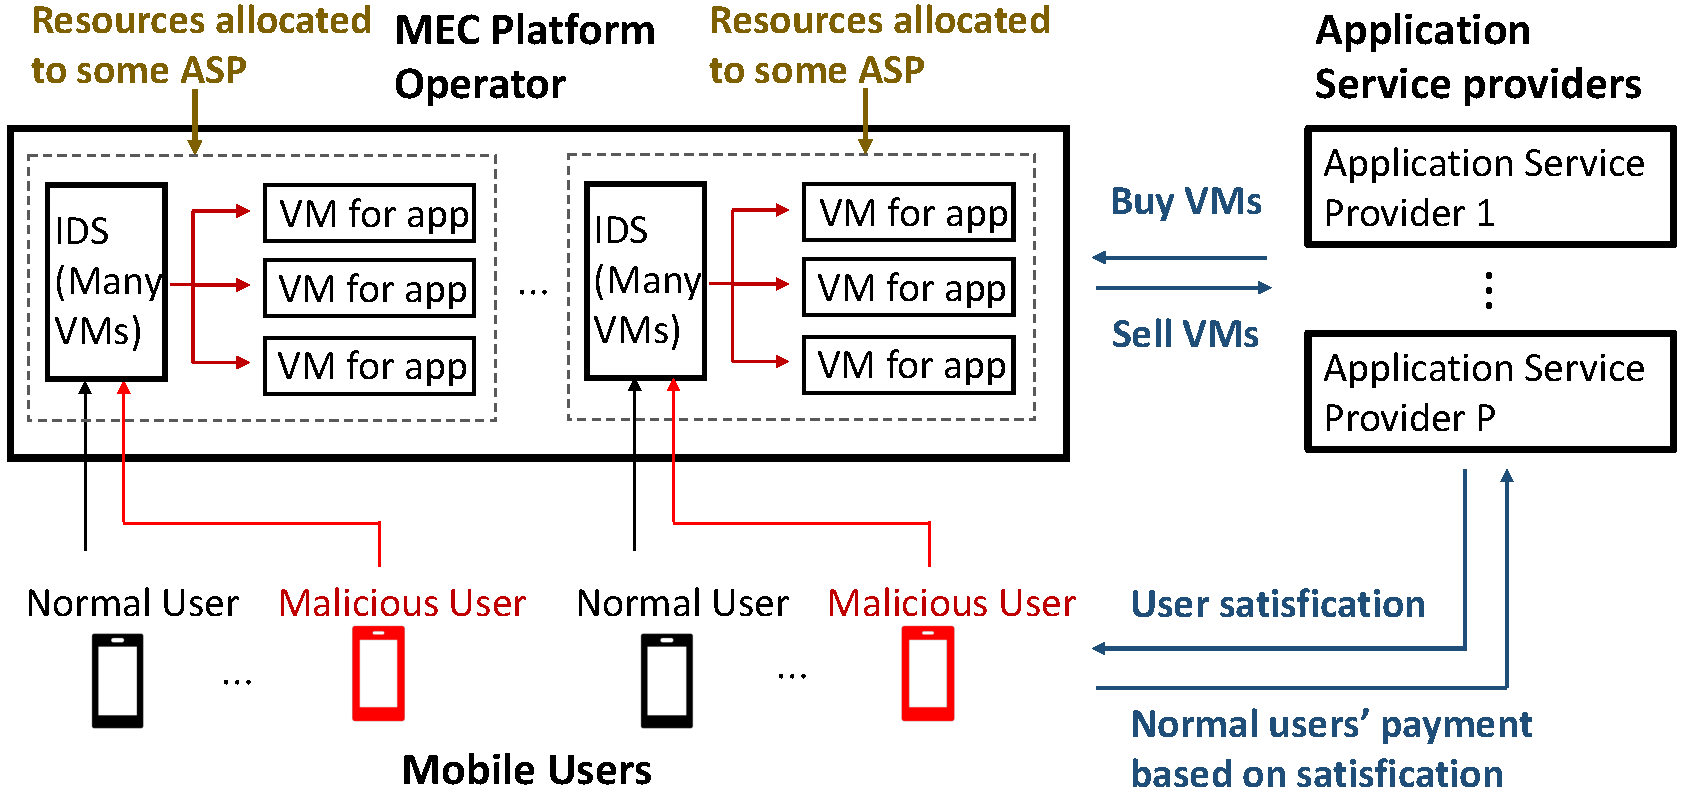
\includegraphics[width= 0.6\columnwidth]{5GDDoS_Game_system_architecture.pdf}
\caption{System Architecture}
\label{fig:system}
\end{figure}

% \begin{table*}[!t]
% \centering
% \caption{Table of Important Notations}
% \label{notationlist}
% \footnotesize
% \begin{tabular}{ |p{0.08\textwidth} |p{0.36\textwidth} || p{0.08\textwidth} |p{0.36\textwidth}|} \hline
%  Notation & Description & Notation & Description \\ \hline
%  $\mathcal{I}$ & set of ASPs & $\mathrm{U}_i$ & set of total EUs of ASP $i$ \\ \hline
%  $\mathrm{U}_i^n$ & set of normal EUs of ASP $i$ & $\mathrm{U}_i^m$ & set of malicious EUs of ASP $i$ \\ \hline
%  $\lambda_{ij}$ & total arrival rate of tasks of EUs of ASP $i$ & $\lambda_{ij}^m$ & malicious arrival rate of tasks of EUs of ASP $i$ \\ \hline
%  $d_{ij}$ & delay requirements of EU $j$ of ASP $i$ & $s_{ij}$ & task size of EU $j$ of ASP $i$ \\ \hline
%  $\chi_{ij}$ & required CPU cycles of EU $j$ of ASP $i$ & $\nu$ & the efficiency of IPS VM \\ \hline
% $H_i(z_i^h)$ & total intercepted malicious requests of ASP $i$ & $\Psi_m^v$ & price per VM from MPO \\ \hline
%  $T_{ij}^t$ & transmission delay from EU $j$ to ASP $i$ & $\mu_i^v$ & mean service rate of ASP $i$ \\ \hline
%  $z_i^h$ & quantity of deployed IPS VM of ASP $i$ &  $z_i^v$ & quantity of purchased VM of ASP $i$ \\ \hline
%  $a_i, b_i$ & lower and upper boundaries of the uniform distribution of delay requirements of ASP $i$ & $\xi_i$ & minimum ratio of VM reserved for application services of ASP $i$  \\ \hline
%  $\gamma_i$ & minimum gap between $\mu_i^v$ and $\lambda_i$ of ASP $i$ & $\eta_i$ & the interception rate of ASP $i$ \\ \hline
% \end{tabular}
% \end{table*}

\begin{table}[!t]
\centering
\caption{Table of Important Notations}
\label{notationlist}
\footnotesize
\begin{tabular}{|p{0.12\columnwidth} |p{0.8\columnwidth}|} \hline
 Notation & Description \\ \hline
 $\mathcal{I}$ & set of ASPs \\ \hline
 $\mathrm{U}_i$ & set of total EUs of ASP $i$ \\ \hline
 $\mathrm{U}_i^n$ & set of normal EUs of ASP $i$ \\ \hline
 $\mathrm{U}_i^m$ & set of malicious EUs of ASP $i$ \\ \hline
 $\lambda_{ij}$ & total arrival rate of tasks of EUs of ASP $i$ \\ \hline $\lambda_{ij}^m$ & malicious arrival rate of tasks of EUs of ASP $i$ \\ \hline
%  $d_{ij}$ & delay requirements of EU $j$ of ASP $i$ \\ \hline
 $s_{ij}$ & task size of EU $j$ of ASP $i$ \\ \hline
 $\chi_{ij}$ & required CPU cycles of EU $j$ of ASP $i$ \\ \hline
 $\nu$ & the efficiency of IPS VM \\ \hline
$H_i(z_i^h)$ & total intercepted malicious requests of ASP $i$ \\ \hline
$\Psi_m^v$ & price per VM from MPO \\ \hline
 $T_{ij}^t$ & transmission delay from EU $j$ to ASP $i$ \\ \hline
 $\mu_i^v$ & mean service rate of ASP $i$ \\ \hline
 $z_i^h$ & quantity of deployed IPS VM of ASP $i$ \\ \hline
 $z_i^v$ & quantity of purchased VM of ASP $i$ \\ \hline
 $a_i, b_i$ & lower and upper boundaries of the uniform distribution of delay requirements of ASP $i$ \\ \hline
 $\xi_i$ & minimum ratio of VM reserved for application for ASP $i$  \\ \hline
 $\gamma_i$ & minimum gap between $\mu_i^v$ and $\lambda_i$ of ASP $i$ \\ \hline
 $\eta_i$ & the interception rate of ASP $i$ \\ \hline
\end{tabular}
\end{table}

We illustrate our system architecture in Fig~\ref{fig:system}. There are three types of entities in our system: the MEC platform operator (MPO), application service providers (ASPs), and end-users (EUs). The MPO manages the computational resources in terms of virtual machines (VMs) of geographically distributed edge servers. Since the ASPs do not have the computational resources to process the application tasks, they have intense demands for the MPO's VM whose total number is $\mathcal{Q}_{V}$. The goal of the MPO is to maximize its profit by finding the optimal unit selling price $\Psi_{m}^v$ per VM. We denote the set of ASPs as $\mathcal{I}=\{1, \cdots, I\}$. The ASPs determine the number of VMs to buy from MPO to maximize profit. We use $z_i^v$ to denote the number of VM bought by the $i$th ASP. Because of the potential network attacks, they utilize these purchased VMs to either run the application service or mitigate the DDoS security attacks. As for the era of B5G/6G, the available network bandwidth is expected to be sufficient to handle massive simultaneous requests. Thus, the main target of DDoS attacks will be the service loading of ASP's server deployed on the VM. In this work, we consider the Application layer DDoS attacks, such as HTTP flooding attacks. When these kinds of DDoS attacks occur, the malicious requests flood into ASPs and exhaust the server's computational resources. Because the VM can be used for main service or IPS, there will be a trade-off when deploying VMs. If ASPs devote most of their VMs to running the application service, they are prone to DDoS security attacks. The security threat would damage the users' quality of experience (QoE) or even paralyze the application service such that the revenue of the ASP will be affected. On the other hand, if the ASPs devote most of their VMs to mitigating the DDoS attack, they can not ensure good satisfaction to the users (e.g., users' latency requirements can not be satisfied) even though the ASPs are immune from the DDoS attacks. Therefore, it is crucial to find an optimal resource allocation between running the application service and mitigating the DDoS attacks.

We denote the set of EUs associated with ASP $i \in \mathcal{I}$ as $\mathrm{U}_i$ and further categorize it into two kinds: normal users (NUs) $\mathrm{U}_i^n$ and malicious users (MUs) $\mathrm{U}_i^m$. We assume that the numbers of normal users and malicious users are estimated in advance and remain the same amounts in the considered operation time period. Each EU $j \in \mathrm{U}_i$ has the Poisson task arrival rate $\lambda_{ij}$, latency requirement $d_{ij}$, and task size $s_{ij}$. We consider that the EUs do not have enough computational resources or needed resources such as Graphics Processing Unit (GPU) to process the application tasks. Therefore, they will offload the tasks to the MPO. The MUs, on the other hand, will launch attacks by sending malicious requests to the edge server. The DDoS attacks occur when the MUs flood into the edge servers. 

The ASPs can intercept some malicious requests by employing intrusion prevention systems (IPS) such as Suricata \cite{Suricata}. The IPS of all ASPs monitors and filters task requests, and all VMs devoted to running the application service process the filtered task requests. We also assume the IPS does not classify the normal task requests as malicious, but it can not discern all malicious requests. The number of malicious requests the IPS filter depends on the number of VMs the ASPs dedicate to the IPS. 

We use $H(\cdot)$ to represent the relationship between the quantity of intercepted malicious requests and the number of devoted VMs. Without losing generality, we assume that the $H(\cdot)$ function to be non-decreasing and concave. Also, $H(0)=0$. When all malicious requests are intercepted, the ASP cannot intercept more malicious requests by deploying more IPS VMs. Therefore, the value of $H(x)$ reaches the number of malicious requests and remains this maximal value when $x$ is larger than a certain value. Inspired by the experiment results in the work\cite{chi}, where the packet delivery rate is proportional to the CPU utilization percentage. We assume that a VM can filter $\nu$ packets. Also, we assume that the malicious packets are uniformly distributed. We define the interception rate, which is the quantity of malicious requests that an IPS VM in the $i$th ASP can intercept. We use $\eta_i$ to denote the interception rate, where $\eta_i$
\begin{equation}
   \begin{aligned}
    \eta_i = \frac{\lambda_i^m}{\lambda_i} \times \nu
    \end{aligned} 
\end{equation}
The term $\lambda_i^m$ indicates the malicious arrival rate of ASP $i$, and $\lambda_i$ indicates the total arrival rate of ASP $i$.

In this paper, we use the $H_i(x)$ function to indicate the relationship between the number of devoted IPS VMs of the $i$th ASP and the number of intercepted malicious requests with a linear form of
\begin{equation}
\begin{aligned}
    H_i(x) = min(\eta_i{x}, \lambda_i^m)
\end{aligned}
\end{equation}

We consider orthogonal frequency-division multiple access (OFDMA) system. The bandwidth of the edge servers whose computational resources are allocated to ASP $i$ denoted by $B_i$ can be divided into $|\mathrm{U}_i|$ sub-bands of size, and each sub-band $W_{i} = B_i/|\mathrm{U}_i|$. Each EU $j\in \mathrm{U}_i$ transmits the data over each of $|\mathrm{U}_i|$ sub-bands, so they would not cause interference to other EUs while transmitting. The uplink transmission rate $R_{ij}$ between ASP $i$ and EU $j \in \mathrm{U}_i$ is
\begin{equation} \label{eqn:shannon}
R_{ij}=W_i \cdot log_2\Big(1+\frac{p_{ij}g_{ij}}{N_{0}}\Big)
\end{equation}
where $p_{ij}$ is the transmission power of EU $j$ in $\mathrm{U}_i$, $g_{ij}$ denotes the uplink channel gain between ASP $i$ and EU $j$, $N_0$ is the background noise power. Based on this rate, we can calculate the mean transmission time of workload consisting of tasks with size $s_{ij}$ from EU $j \in \mathrm{U}_i$ to ASP $i$.
\begin{equation}
T_{ij}^t=\frac{\lambda_{ij} \cdot s_{ij}}{R_{ij}}
\end{equation}

The task arrival processes at ASP $i$, which are offloaded from the EUs, also follow the Poisson process according to the Poisson process's stationary property. Furthermore, the mean arriving rate of the Poisson process at ASP $i$ can be expressed as $\lambda_i = \sum_{j \in \mathrm{U}_i} \lambda_{ij}$ based on the superposition property of the Poisson process. We use $\lambda_i^m$ to indicate the total arrival rate of malicious request, which is expressed as $\lambda_i^m = \sum_{j \in \mathrm{U}_i^m} \lambda_{ij}$. Similarly, we define the total arrival rate of normal request as $\lambda_i^n$, where $\lambda_i^n =  \sum_{j \in \mathrm{U}_i^n} \lambda_{ij}$. Since the ASPs buy VMs from MPO, whose overall computational resources are still limited compared to the cloud platform such as Google cloud platform or Amazon EC2 platform, we model the meaning processing delay of all VMs purchased by ASPs using $M/M/1$ queue. Each VM of MPO is homogeneous and can process $f_m^v$ CPU cycles per second. As the average required CPU cycles for a task of ASP $i$ may be different, the mean service rate of the queue at ASP $i$ denoted by $\mu_i^v$ (the number of tasks that a VM can process on average per second) is different for every ASP $i$. We denote the required CPU cycles of user $j \in \mathsf{U}_i$ as $\chi_{ij}$. The relationship between $f_m^v$ and $\mu_i^v$ is
\begin{equation}\label{eqn:service_rate}
\mu_i^v = f_m^v/(\frac{\sum_{j \in \mathsf{U}_i} \chi_{ij}}{|\mathrm{U}_i|})
\end{equation}
Furthermore, we let $\chi_{ij} = B \times s_{ij}$, where $B$ is the coefficient of the linear relationship between $s_{ij}$ and $\chi_{ij}$.
% \begin{equation}\label{eqn:required_cpu}
% \chi_{ij} = B \times s_{ij}
% \end{equation}

If the ASP $i$ devotes $z_i^h$ out of $z_i^v$ VMs to IPS, the intercepted quantity of malicious requests is $H_i(z_i^h)$. When ASP $i$ buys $z_i^v$ VMs from the MPO and devotes $z_i^h$ to IPS, those VMs' mean processing delay is
\begin{equation} \label{eqn:asp_mm1_delay}
T_i^p(z_i^v, z_i^h) = \frac{1}{(z_i^v - z_i^h)\mu_i^v - \big(\lambda_i - H_i(z_i^h)\big)}
\end{equation}
where $(z_i^v - z_i^h)$ is the number of VMs devoted to serving EUs, and $(z_i^v - z_i^h)\mu_i^v$ is the total service rate of ASP $i$. Moreover, the $H_i(z_i^h)$ is the number of intercepted requests, and $(\lambda_i - H_i(z_i^h))$ is the number of processed requests.

The payment from the NU $j \in \mathrm{U}_i^n$ to the ASP $i$ depends on whether the latency requirements $d_{ij} \, \forall j \in \mathrm{U}_i^n$ are satisfied or not. If latency requirements $d_{ij}$ are met, NU $j \in \mathrm{U}_i^n$ pays a price $\Psi_{ij}$ to ASP $i$. The heterogeneity of the payment reflects the different characteristics of NUs. The NUs with different latency requirements may have different level of satisfaction with the same service provided by the ASP $i$. If latency requirements $d_{ij}$ are not met, NU $j \in \mathrm{U}_i^n$ does not pay ASP $i$. The MUs $j \in \mathrm{U}_i^m$ will not pay ASP $i$ no matter whether their latency requirement are satisfied or not. We represent the payment of NU $j \in \mathrm{U}_i$ as follows:
\begin{subnumcases}{\mathcal{K}_{ij}(z_i^v, z_i^h)=\label{eqn:devicepayment}}
  \Psi_{ij} & \hspace*{-1.7mm}if $T_{ij}^t + T_i^p(z_i^v, z_i^h) \leq d_{ij}$, $j \in \mathrm{U}_i^n$\\
  0 & \hspace*{-1.7mm}if $T_{ij}^t + T_i^p(z_i^v, z_i^h) > d_{ij}$, $j \in \mathrm{U}_i^n$ \\
  0 & \hspace*{-1.7mm}$j \in \mathrm{U}_i^m$
\end{subnumcases}

\section{Game Formulation}\label{sec:game_formulations}
Because of the rationalities of both MPO and ASPs, the intrinsic hierarchy between MPO and ASPs, and the influence of one ASP's action on other ASPs' profits, we model the interaction between MPO and ASPs as a two-stage single-leader-multi-followers Stackelberg game. Both the MPO and ASPs are rational players and have the ultimate goal of maximizing their profit by choosing their actions. The MPO can select a price per VM $\Psi_{m}^v$ that maximizes its profit, and each ASP $i$ determines the number of VMs to buy from MPO $z_i^v$ to optimize its profit too. The MPO's selection of price per VM affects how many VMs those ASPs would buy, which impacts its revenue. Since the ASPs need to buy the computational resources from MPO to maintain their application services, the MPO has an advantage over the ASPs. Moreover, due to MPO's finite number of VMs, the more one ASP buys, the less other ASPs can buy. The action of one ASP affects other ASPs' profit. The Stackelberg game where the MPO acts as the leader and all ASPs are the followers can capture such coupled and hierarchical relationships between MPO and ASPs, the self-interests of both MPO and ASPs, and the implicit influence among ASPs. Thus, we first illustrate the actions and utilities of MPO and ASPs and then formulate the optimization problems for both players as follows.

\subsection{The Action and The Utility of ASPs}
Given the MPO's price per VM $\Psi_m^v$, each ASP $i$ chooses the number of VMs to buy from the MPO $z_i^v$ to maximize its profit which is the revenue accrued from the normal MU $j \in \mathrm{U}_i^n$ minus the payment to the MPO for purchasing $z_i^v$ VMs. The natural candidate for the utility is profit. However, even with the same $z_i^v$, the revenue of ASP $i$ hinges on how many VMs it dedicates to the IPS, the distribution of latency requirements $d_{ij}$, and the different payments of heterogeneous NU $j \in \mathrm{U}_i^n$. We define the utility of ASP $i$ when it purchases $z_i^v$ VMs from MPO as the maximum expected profit across the different number of VMs dedicated to the IPS $z_i^h$ with respect to the distribution of latency requirement $d_{ij}$. Furthermore, we assume that the latency requirements $d_{ij} \, \forall j \in \mathrm{U}_i$ follow an uniform distribution indexed by $i$ over interval $[a_i, b_i]$ denoted by $\mathcal{U}(a_i,b_i)$. To make the problem tractable, we relax the variables $z_i^v, z_i^h \, \forall i \in \mathcal{I}$ to real numbers. The utility of ASP $i$ given $\Psi_m^v$ is
\begin{align}
&Y_i(z_i^v|\Psi_m^v) \triangleq \max_{z_i^h} \mathsf{E}_{d_{ij}}\Big[\sum_{j \in \mathrm{U}_i^n} \mathcal{K}_{ij}(z_i^v, z_i^h) - \Psi_m^v z_i^v\Big] 
\hspace*{-1mm}
\iffalse=\max_{z_i^h} \mathsf{E}_{d_{ij}}[\sum_{j \in \mathrm{U}_i^n}\Psi_{ij}\mathds{1}\{T_{ij}^t + T_i^p(z_i^v, z_i^h) \leq d_{ij}\} - \Psi_m^vz_i^v] \nonumber \fi\\
\hspace*{-1mm}&=\max_{z_i^h} [\sum_{j \in \mathrm{U}_i^n}\Psi_{ij}(1-F_{d_{ij}}(T_{ij}^t+T_i^p(z_i^v, z_i^h)) - \Psi_m^vz_i^v] \\ %\label{eqn:asp_def_subobjective_unfold}
&\hspace*{-1mm}\triangleq \max_{z_i^h} X_i(z_i^h|z_i^v,\Psi_m^v) \label{eqn:asp_def_subobjective}
\end{align}
where $F_{X}(x)$ is the cumulative distribution function (CDF).
% of $\mathcal{U}(a_i,b_i)$.
% \begin{subnumcases}{F_X(x)=\label{eqn:CDF}}
%   0 & $x < a_i$\\
%   \frac{x-a_i}{b_i-a_i} &  $x \in[a_i, b_i]$\\
%   1 & $x > b_i$
% \end{subnumcases}

The $\mathsf{E}_{d_{ij}}$ is derived by taking expectation with respect to the distribution of $d_{ij}$, where $\mathds{1}\{\cdot\}$ is the indicator function. The $F_{d_{ij}}(T_{ij}^t+T_i^p(z_i^v, z_i^h))$ is the probability that the latency requirement $d_{ij}$ of the NU $j\in\mathrm{U}_i^n$ are not satisfied, which is also the CDF of $\mathcal{U}(a_i,b_i)$. Given $z_i^v$, we have three constraints on $z_i^h$. First, the number of VMs dedicated to IPS $z_i^h$ must be no larger than the number of purchased VMs $z_i^v$. Second, to make the processing queue stable, the mean service rate by VMs dedicated to running the service must be higher than the mean arrival rate for EUs $j \in \mathrm{U}_i$. Third, we introduce $\xi_i\in[0, 1]$ as a resource reservation constraint to control the minimum resource reserved for the service. Thus, to define the utility of ASP $i$ when the purchased VMs from the MPO is $z_i^v$, we have to solve the following optimization problem to determine the optimal configuration of IPS first.
\begin{maxi!}[2]
  {z_i^h \in \mathbb{R}}
  {X_i(z_i^h|z_i^v,\Psi_m^v) \label{eqn:asp_utility_def_opti_obj}}
  {\label{eqn:asp_utility_def_opti}}
  {}
  \addConstraint{0 \leq z_i^h \leq \xi_i z_i^v}{\label{eqn:asp_utility_def_opti_const1}}
  \addConstraint{0 < (z_i^v-z_i^h)\mu_i^v - \lambda_i + H_i(z_i^h) }{\label{eqn:asp_utility_def_opti_const2}}
\end{maxi!}
%In (\ref{eqn:asp_utility_def_opti_const1}), we further introduce a system parameter $\xi_i\in[0, 1]$ to control the feasible range of $z_i^h$.
The observation that both (\ref{eqn:asp_utility_def_opti_const1}) and (\ref{eqn:asp_utility_def_opti_const2}) impose upper bounds on the range of $z_i^h$ will simplify the characterization of the optimal $z_i^h$. 

Showing the $Y_i(z_i^v)$ is well-defined is equivalent to proving the optimization problem (\ref{eqn:asp_utility_def_opti}) has at least one solution. \footnote{If there are multiple optimal points having same values of $X_i(z_i^h|z_i^v,\Psi_m^v)$, we randomly select one as the solution to (\ref{eqn:asp_utility_def_opti}).} For convenience, we rewrite the term $\sum_{j \in \mathrm{U}_i^n}\Psi_{ij}(1-F_{d_{ij}}(T_{ij}^t+T_i^p(z_i^v, z_i^h))$ using the definition of $F_{d_{ij}}(T_{ij}^t+T_i^p(z_i^v, z_i^h))$, so it becomes\footnote{In the rest of the paper, we assume that the $T_{ij}^t+T_i^p(z_i^v, z_i^h)$ lies in the range of $[a_i, b_i]$, so we assume $\mathrm{U}_i^{n2} = \mathrm{U}_i^{n}$.}
\begin{equation}
\begin{aligned}
&\sum_{j \in \mathrm{U}_i^{n1}}\Psi_{ij} \times 1 +\sum_{j \in \mathrm{U}_i^{n2}}\Psi_{ij} \times &(1-\frac{T_{ij}^t+T_i^p(z_i^v, z_i^h)-a_i}{b_i-a_i}) \\
% & + \sum_{j \in \mathrm{U}_i^{n3}}\Psi_{ij} \times 0
\end{aligned}
\end{equation}
, where we divide $\mathrm{U}_i^{n}$ into three sets $\mathrm{U}_i^{n1}$, $\mathrm{U}_i^{n2}$ and $\mathrm{U}_i^{n3}$.
We define these three sets as 
\begin{subequations}\label{normal_set_user}
\begin{align}
\mathrm{U}_i^{n1} =& \{T_{ij}^t+T_i^p(z_i^v, z_i^h) < a_i\ |\ j \in \mathrm{U}_i^{n}\}\label{normal_set_user_1} \\
\mathrm{U}_i^{n2} =& \{a_i \leq T_{ij}^t+T_i^p(z_i^v, z_i^h) \leq b_i\ |\ j \in \mathrm{U}_i^{n}\}\label{normal_set_user_2} \\
\mathrm{U}_i^{n3} =& \{ b_i < T_{ij}^t+T_i^p(z_i^v, z_i^h) \ |\ j \in \mathrm{U}_i^{n}\}\label{normal_set_user_3}
\end{align}
\end{subequations}
\begin{lemma}
The utility of ASP $i$, $Y_i(z_i^v)$, is well defined, as the optimization problem (\ref{eqn:asp_utility_def_opti}) is a convex optimization problem and has at least one optimal point 
\end{lemma}
The detailed proof is deferred in Appendix \ref{appendix:lemma_1}.
% \begin{proof}
% The feasible region imposed by (\ref{eqn:asp_utility_def_opti_const1}) and (\ref{eqn:asp_utility_def_opti_const2}) is a closed and bounded interval in $\mathbb{R}$ and thus is a convex set. As the objective function (\ref{eqn:asp_utility_def_opti_obj}) is continuous in $z_i^h$, the existence of the optimal solution then comes from the Extreme Value Theorem. If (\ref{eqn:asp_utility_def_opti_obj}) is concave at each feasible $z_i^h$, optimization problem (\ref{eqn:asp_utility_def_opti}) is a convex optimization problem. It remains to show that the objective function (\ref{eqn:asp_utility_def_opti_obj}) is concave in feasible $z_i^h$. By rearranging the terms, we express $X_i(z_i^h|z_i^v,\Psi_m^v)$ as
% \begin{equation}
% \begin{aligned}
%     \sum_{j \in \mathrm{U}_i^{n}}\Psi_{ij}(1-\frac{T_{ij}^t+T_i^p(z_i^v, z_i^h)-a_i}{b_i-a_i})- \Psi_m^v z_i^v 
% \end{aligned}
% \end{equation}
% To show $X_i(z_i^h|z_i^v,\Psi_m^v)$ is concave in feasible $z_i^h$, it suffices to show that $T_i^p(z_i^v, z_i^h)$ is convex in feasible $z_i^h$. We will verify the convexity of $T_i^p(z_i^v, z_i^h)$. From (\ref{eqn:asp_mm1_delay}), We can rewrite it as
% \begin{equation} 
% \begin{aligned}
% T_i^p(z_i^v)=\frac{1}{(z_i^v-z_i^h)\mu_i^v - \lambda_i + H_i(z_i^h)}
% \end{aligned}
% \end{equation}
% By definition, $H_i(z_i^h)$ is concave in feasible $z_i^h$. In addition, $(z_i^v-z_i^h)\mu_i^v - \lambda_i$ is an affine function of $z_i^h$, so $(z_i^v-z_i^h)\mu_i^v - \lambda_i + H_i(z_i^h)$ is concave in feasible $z_i^h$. Given a positive concave function $f(x)$ in feasible $x$, $\frac{1}{f(x)}$ is convex in feasible $x$\cite[Chapter~3.2]{boyd2004convex}. Thus, $T_i^p(z_i^v, z_i^h)$ is convex in feasible $z_i^h$ and $X_i(z_i^h|z_i^v,\Psi_m^v)$ is concave in feasible $z_i^h$.
% \end{proof}

After defining the utility of ASP $i$, $Y_i(z_i^v)$, we can now formulate the optimization problem of ASP $i$ given the MPO's price per VM $\Psi_m^v$.
\begin{maxi!}[2]
  {z_i^v \in \mathbb{R}}
  {Y_i(z_i^v|\Psi_m^v) \label{eqn:asp_utility_opti_obj}}
  {\label{eqn:asp_utility_opti}}
  {}
  \addConstraint{\lambda_i+ \gamma_i \leq z_i^v \mu_i^v}{\label{eqn:asp_utility_opti_const1}}
  \addConstraint{0 \leq Y_i(z_i^v|\Psi_m^v)}{\label{eqn:asp_utility_opti_const2}}
\end{maxi!}
The constraint (\ref{eqn:asp_utility_opti_const1}) regulates that when the ASP $i$ dedicates all purchased VMs to running the application service, the mean service rate must be larger than the mean arrival rate by at least $\gamma_i$, where $\gamma_i\geq 0$. The constraint (\ref{eqn:asp_utility_opti_const1}) also ensures that the feasible region of (\ref{eqn:asp_utility_def_opti}) is non-empty because under this constraint, there is at least one $z_i^h$ that satisfies (\ref{eqn:asp_utility_def_opti_const2}). The constraint (\ref{eqn:asp_utility_opti_const2}) represents the individual rationality for every ASP. That is, when making the processing queue stable gives a negative utility, the ASPs would rather choose not to serve the users and not buy any VMs from the MPO, which has zero utility. We defer the analysis of solutions to both optimization problems (\ref{eqn:asp_utility_def_opti}) and (\ref{eqn:asp_utility_opti}) to \Cref{sec:game_optimization}. We denote the solution to (\ref{eqn:asp_utility_opti}) as $(z_i^v(\Psi_m^v))^*$ to emphasize the dependence on the MPO's price per VM $\Psi_m^v$.

\subsection{The Action and The Utility of The MPO}
With the prediction about the number of VMs purchased by ASPs $(z_i^v(\Psi_m^v))^* \, \forall i \in \mathcal{I}$, the MPO chooses the price per VM $\Psi_m^v$ to maximize its utility which is defined as the MPO's profit. The revenue of the MPO is the sum of payments from all ASPs. Although the ASPs buy those VMs from the MPO, it is the infrastructure of the MPO that processes the application requests. As a result, the MPO has an operating cost for keeping the VMs working. We represent the cost for operating $\sum_{i \in \mathcal{I}} (z_i^v(\Psi_m^v))^*$ VMs by $C_m^v\big(\sum_{i \in \mathcal{I}} (z_i^v(\Psi_m^v))^*\big)$. The function $C_m^v(\cdot)$ is assumed to be convex and non-decreasing. We denote the MPO's utility as $Y_m(\Psi_m^v)$ and formulate the MPO's optimization problem.
\begin{maxi!}[2]
  {\Psi_m^v}
  {\Psi_m^v \cdot \sum_{i \in \mathcal{I}} (z_i^v(\Psi_m^v))^* - C_m^v\big(\sum_{i \in \mathcal{I}} (z_i^v(\Psi_m^v))^*\big) \label{eqn:mpo_utility_opti_obj}}
  {\label{eqn:mpo_utility_opti}}
  {}
  \addConstraint{\sum_{i \in \mathcal{I}} (z_i^v(\Psi_m^v))^* \leq \mathcal{Q}_v}{\label{eqn:mpo_utility_opti_const1}}
  \addConstraint{0 \leq \Psi_m^v}{\label{eqn:mpo_utility_opti_const2}}
\end{maxi!}
The constraint (\ref{eqn:mpo_utility_opti_const1}) mandates the maximum number of VMs $\mathcal{Q}_v$ the MPO can sell. The constraint (\ref{eqn:mpo_utility_opti_const1}) imposes a lower bound for MPO's price per VM. The constraint (\ref{eqn:mpo_utility_opti_const2}) requires the MPO's price per VM must be non-negative. The property of this optimization (\ref{eqn:mpo_utility_opti}) relies on the solution $(z_i^v(\Psi_m^v))^*$, and we defer the analysis to \Cref{sec:game_optimization}.

\begin{figure}
    \centering
    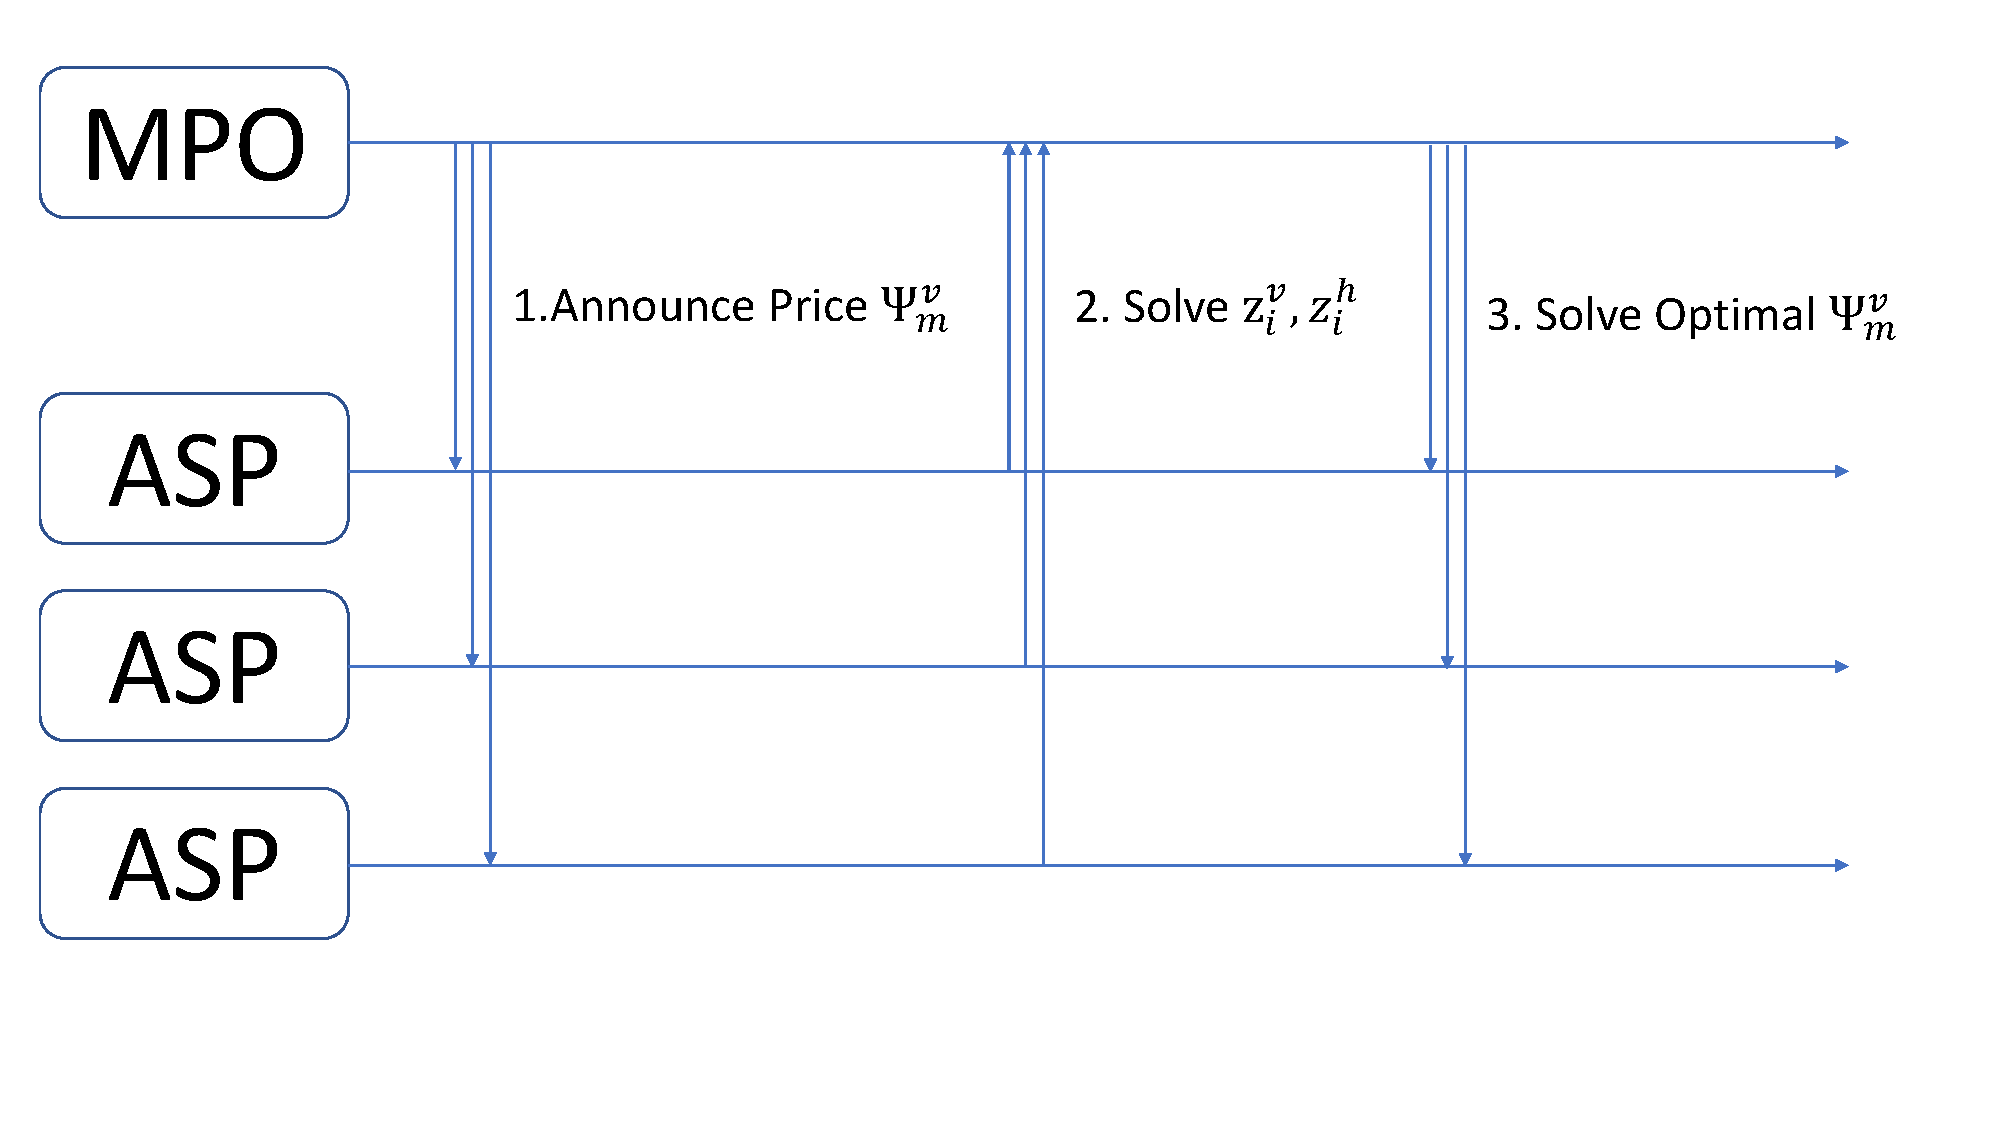
\includegraphics[width=0.6\columnwidth]{5GDDoS_Game_Flow_Chart.pdf}
    \caption{Flow Chart of the Proposed Stackelberg Game}
    \label{fig:flow_chart}
\end{figure}

\section{Game Optimization} \label{sec:game_optimization}
We would leverage the backward induction principle to derive the Stackelberg equilibrium of the formulated Stackelberg game. That is, we solve the followers' (ASPs') optimization problems first and then the leader's (the MPO's) optimization problem based on the expected best responses of ASPs to the MPO's price per VM, i.e., $(z_i^v(\Psi_m^v))^* \, \forall i \in \mathcal{I}$. 

We formally define the Stackelberg equilibrium \cite{bacsar1998dynamic} of our proposed Stackelberg game. We symbolize the ASP $i$'s action set using $\mathcal{A}_i$ and the profile of all ASPs' action using $\bm{z^v}=(z_1^v, z_2^v, \cdots, z_I^v) \in \mathcal{A}_1 \times \mathcal{A}_2 \cdots \times \mathcal{A}_I$ where $\mathcal{A}_1 \times \mathcal{A}_2$ means the Cartesian product of $\mathcal{A}_1$ and $\mathcal{A}_2$. The ASP $i$'s best response set $\mathcal{B}_i^R(\Psi_m^v)$ to the MPO's price per VM $\Psi_m^v$ is 
\begin{equation} \label{eqn:asp_best_response}
\begin{aligned}
&\mathcal{B}_i^R(\Psi_m^v) = \{z_i^v \in \mathcal{A}_i |Y_i(z_i^v|\Psi_m^v) \geq Y_i\big((z_i^v)'|\Psi_m^v\big) \\
&\forall (z_i^v)' \in \mathcal{A}_i, (z_i^v)' \neq z_i^v\}
\end{aligned}
\end{equation}
We also denote the Cartesian product of all ASPs' best response sets as
\begin{equation}
\mathcal{B}^R(\Psi_m^v) = \mathcal{B}_1^R(\Psi_m^v) \times \mathcal{B}_2^R(\Psi_m^v) \cdots \times \mathcal{B}_I^R(\Psi_m^v)
\end{equation}
Likewise, we denote the MPO's action set as $\mathcal{A}_m$. Furthermore, to stress the influence of ASPs' actions on the MPO's utility, we use $Y_m(\Psi_m^v|\bm{z^v})$ to represent the MPO's utility in the following definition of the MPO's best response set.
\begin{equation} \label{eqn:mpo_best_response}
\begin{aligned}
\mathcal{B}_m = &\{\Psi_m^v \in \mathcal{A}_m| Y_m(\Psi_m^v|\bm{z^v}) \geq Y_m((\Psi_m^v)'|(\bm{z^v})') \\
&\forall (\Psi_m^v)' \in \mathcal{A}_m, (\Psi_m^v)' \neq \Psi_m^v, \forall \bm{z^v} \in \mathcal{B}^R(\Psi_m^v) \\
&\forall  (\bm{z^v})' \in \mathcal{B}^R\big((\Psi_m^v)'\big)\}
\end{aligned}
\end{equation}
\begin{definition}[\textbf{Stackelberg equilibrium}] \label{def:stackelberg_equilibrium}
If $\mathcal{B}_{m}$ and $\mathcal{B}^R(\Psi_m^v)$ are both non-empty, the Stackelberg equilibrium in our mechanism is a vector of dimension $(I+1)$ that is an element of $\mathcal{B}_m  \times \mathcal{B}^R(\Psi_m^v)$.
\end{definition}

We analyze the process of the formulated Stackelberg game according to whether the solution to (\ref{eqn:asp_utility_def_opti}) is the extreme point or boundary point of the constraint.

\subsection{ASP Optimization Problem}
\textbf{Case 1}: The optimal point of (\ref{eqn:asp_utility_def_opti}) is the extreme point whose first derivative with respect to $z_i^h$. The first derivative of $X_i(z_i^h|z_i^v,\Psi_m^v)$ with respect to $z_i^h$ is
\begin{equation} \label{eqn:asp_utilitu_def_firstderiv}
[(z_i^v - z_i^h) - \lambda_i + H_i(z_i^h)]^{-2} \cdot (-\mu_i^v + H_i'(z_i^h))
\end{equation}
% $(z_i^v - z_i^h) - \lambda_i + H_i(z_i^h)$ is positive at every feasible $z_i^h$ because of the constraint (\ref{eqn:asp_utility_def_opti_const2}). Also, $H'(\cdot)$ is non-decreasing and thus has an inverse function denoted by $G(\cdot)$. We can solve the extreme point denoted by $(z_i^h)^*$ through letting (\ref{eqn:asp_utilitu_def_firstderiv}) equal zero.
% \begin{equation} \label{eqn:asp_utility_def_extreme_point}
% (z_i^h)^* = (H')^{-1}(\mu_i^v) \triangleq G(\mu_i^v)
% \end{equation}
% When we substitute (\ref{eqn:asp_utility_def_extreme_point}) into (\ref{eqn:asp_mm1_delay}), the mean processing delay denoted as $T_{i,1}^p(z_i^v)$ depends only on $z_i^v$ and is
% \begin{equation}
% T_{i,1}^p(z_i^v) = \frac{1}{\big(z_i^v - G(\mu_i^v)\big)\mu_i^v - \lambda_i + H\big(G(\mu_i^v)\big)}
% \end{equation}
% According to (\ref{eqn:asp_def_subobjective_unfold}) and (\ref{eqn:asp_def_subobjective}), the objective function (\ref{eqn:asp_utility_opti_obj}) becomes
% \begin{equation}\label{eqn:asp_case1_utility}
% \begin{aligned}
% Y_i^1(z_i^v|\Psi_m^v) \triangleq \sum_{j \in \mathrm{U}_i^{n}}\Psi_{ij}(1-\frac{T_{ij}^t + T_{i,1}^p(z_i^v)-a_i}{b_i-a_i}) - \Psi_m^vz_i^v
% \end{aligned}
% \end{equation}


Nevertheless, we can prove that Case 1 will never happen since $H_i(x) = min(\eta_i{x}, \lambda_i^m)$. %We explain the property in the following.
\begin{lemma} \label{lemma:asp_case1_not_exist}
The extreme point of $X_i(z_i^h|z_i^v,\Psi_m^v)$ doesn't exist in feasible $z_i^h$ if $H_i(x) = min(\eta_i{x}, \lambda_i^m)$.
\end{lemma}
The detailed proof is deferred in Appendix \ref{appendix:lemma_2}.

% \begin{proof}
% From (\ref{eqn:asp_utilitu_def_firstderiv}), we substitute $\eta_i{z_i^h}$ into $H_i(z_i^h)$, then we can obtain
% \begin{equation} \label{eqn:asp_utilitu_simplified}
% [(z_i^v - z_i^h) - \lambda_i + \eta_i{z_i^h}]^{-2} \cdot (-\mu_i^v + \eta_i)
% \end{equation}
% Obviously, regardless of the value of $z_i^h$, the (\ref{eqn:asp_utilitu_simplified}) will never be zero. Therefore, the extreme point does not exist.\qedhere
% \end{proof}
Now we know that the extreme point of (\ref{eqn:asp_utility_def_opti_obj}) does not exist in feasible $z_i^h$, so the maximum value of $X_i(z_i^h|z_i^v,\Psi_m^v)$ only happens at the boundary points of feasible $z_i^h$. Moreover, for the linear form of $H_i(x)$, the coefficient $\eta_i$ indicates the number of intercepted malicious requests of an IPS VM. If $\eta_i$ is larger than the service rate $\mu_i^v$, the ASP would tend to deploy as much IPS ratio as it could. In contrast, if $\eta_i$ is smaller than the service rate $\mu_i^v$, the ASP would tend to serve its users instead of intercepting malicious requests. 

\textbf{Case 2}: In this case, the interception rate $\eta_i$ is larger than the service rate $\mu_i^v$ of the ASP $i$. As a result, the ASP has more incentive to deploy as many IPS VMs as they could. In this situation, the optimal point of (\ref{eqn:asp_utility_def_opti}) is the right boundary of (\ref{eqn:asp_utility_def_opti_const1}) or the exact number of VMs required to defend all of the malicious requests. With a specific form of $H_i(x) = min(\eta_i x, \lambda_i^m)$ and the purchased number of VM is $z_i^v$, the ASP $i$'s optimal number of VMs devoted to the IPS is
\begin{equation} \label{eqn:asp_utility_def_first_boundary}
(z_i^h)^* = min(\xi_i z_i^v, \frac{\lambda_i^m}{\eta_i})
\end{equation}

We substitute $(z_i^h)^*$ into (\ref{eqn:asp_mm1_delay}), and the mean processing delay in this case denoted as $T_{i,2}^p(z_i^v)$ is

\begin{subnumcases}{=\label{eqn:asp_case2_mm1_delay}}
  \frac{1}{(1-\xi_i)z_i^v\mu_i^v - \big(\lambda_i - \eta_i \xi_iz_i^v\big)} & $z_i^v<\frac{\lambda_i^m}{\eta_i \xi_i}$ \label{eqn:asp_case2_mm1_delay1} \\
  \frac{1}{(z_i^v-\frac{\lambda_i^m}{\eta_i})\mu_i^v - \big(\lambda_i - \lambda_i^m\big)} & $z_i^v\geq\frac{\lambda_i^m}{\eta_i \xi_i}$ \label{eqn:asp_case2_mm1_delay2}
\end{subnumcases}

According to %(\ref{eqn:asp_def_subobjective_unfold}) and
(\ref{eqn:asp_def_subobjective}), the objective function (\ref{eqn:asp_utility_opti_obj}) becomes
\begin{equation} \label{eqn:asp_case2_objective}
\begin{aligned}
Y_i^2(z_i^v|\Psi_m^v) \triangleq \sum_{j \in \mathrm{U}_i^{n}}\Psi_{ij}(1-\frac{T_{ij}^t + T_{i,2}^p(z_i^v)-a_i}{b_i-a_i}) - \Psi_m^vz_i^v
\end{aligned}
\end{equation}
If $Y_i^2(z_i^v|\Psi_m^v)$ is concave in feasible $z_i^v$, it is much easier to solve the optimization problem (\ref{eqn:asp_utility_opti}) with the objective being $Y_i^2(z_i^v|\Psi_m^v)$. We prove these properties in the following.
\begin{lemma} \label{lemma:asp_case2_utility_concave}
$Y_i^2(z_i^v|\Psi_m^v)$ is concave in feasible $z_i^v$.
\end{lemma}
The detailed proof is deferred in Appendix \ref{appendix:lemma_3}.
% \begin{proof}
% If $T_{i,2}^p(z_i^v)$ is convex in feasible $z_i^v$, $Y_i^2(z_i^v|\Psi_m^v)$ is concave in feasible $z_i^v$. We will verify the convexity of $T_{i,2}^p(z_i^v)$. We can write $T_{i,2}^p(z_i^v)$ as follow
% \begin{equation} \label{eqn:asp_case2_mm1_delay_min}
% \begin{aligned}
% &T_{i,2}^p(z_i^v) = \\ &\frac{1}{(z_i^v-min(\xi_i z_i^v, \frac{\lambda_i^m}{\eta_i}))\mu_i^v - \big(\lambda_i - \eta_i\min(\xi_i z_i^v, \frac{\lambda_i^m}{\eta_i})\big)}
% \end{aligned}
% \end{equation}
% By rewriting (\ref{eqn:asp_case2_mm1_delay_min}), $T_{i,2}^p(z_i^v)$ can be further expressed as
% \begin{equation} \label{eqn:asp_case2_mm1_delay_min_new}
% \begin{aligned}
% T_{i,2}^p(z_i^v) = \frac{1}{z_i^v\mu_i^v - \lambda_i +(\eta_i - \mu_i^v)\min(\xi_i z_i^v, \frac{\lambda_i^m}{\eta_i})}
% \end{aligned}
% \end{equation}
% Since the term $(\eta_i - \mu_i^v)$ is always positive in Case 2, $(\mu_i^v - \eta_i)\min(\xi_i z_i^v, \frac{\lambda_i^m}{\eta_i})$ is positive and concave in feasible $z_i^v$. In addition, $(z_i^v\mu_i^v - \lambda_i)$ is an affine function in feasible $z_i^v$, so $z_i^v\mu_i^v - \lambda_i+(\mu_i^v - \eta_i)\min(\xi_i z_i^v, \frac{\lambda_i^m}{\eta_i})$ is concave in feasible $z_i^v$\cite[Chapter~3.2]{boyd2004convex}.

% Given a concave function $f(x)$ in feasible $x$, $\frac{1}{f(x)}$ is convex in feasible $x$. Therefore, $T_{i,2}^p(z_i^v)$ is convex in feasible $z_i^v$ and $Y_i^2(z_i^v|\Psi_m^v)$ is concave in feasible $z_i^v$.  \qedhere
% \end{proof}

With \Cref{lemma:asp_case2_utility_concave}, we can characterize the solution to the optimization problem (\ref{eqn:asp_utility_opti}). Before stating the result, we define the feasible region of (\ref{eqn:asp_utility_opti_const1}) as $\Upsilon_i$ for ASP i while the feasible region of (\ref{eqn:asp_utility_opti_const2}) as $\Upsilon_i^2$ when the $Y_i(z_i^v|\Psi_m^v)$ equals $Y_i^2(z_i^v|\Psi_m^v)$.
\begin{theorem}\label{thm:asp_case2_optimal}
The solution to the optimization problem (\ref{eqn:asp_utility_opti}) when the objective function (\ref{eqn:asp_utility_opti_obj}) equals $Y_i^2(z_i^v|\Psi_m^v)$ and $H_i(x)=min(\eta_i x, \lambda_i^m)$ is $(z_{i,2}^v(\Psi_m^v))^*$ if $\Upsilon_i \cap \Upsilon_i^2 \neq \emptyset $
\begin{subnumcases}{=\label{eqn:asp_case2_optimal_solution}}
  \frac{\lambda_i+\gamma_i}{\mu_i^v} & $(z_{i,2}^{v,e}(\Psi_m^v))^* < \frac{\lambda_i+\gamma_i}{\mu_i^v}$ \label{eqn:asp_case2_optimal_solution_lower_boundary} \\
  (z_{i,2}^{v,e}(\Psi_m^v))^* & $(z_{i,2}^{v,e}(\Psi_m^v))^* \geq \frac{\lambda_i+\gamma_i}{\mu_i^v}$ \label{eqn:asp_case2_optimal_solution_extreme}
\end{subnumcases}
where $(z_{i,2}^{v,e}(\Psi_m^v))^*$
\begin{subnumcases} {=\label{eqn:asp_case2_utility_extreme}}
(z_{i,2}^{v,e''}(\Psi_m^v))^*
 &if $(z_{i,2}^{v,e'}(\Psi_m^v))^*<\frac{\lambda_i^m}{\eta_i \xi_i}$
\label{eqn:asp_case2_utility_extreme1}\\
(z_{i,2}^{v,e'}(\Psi_m^v))^*
 &if $(z_{i,2}^{v,e'}(\Psi_m^v))^*\geq \frac{\lambda_i^m}{\eta_i \xi_i}$
\label{eqn:asp_case2_utility_extreme2}
\end{subnumcases}
where $(z_{i,2}^{v,e'}(\Psi_m^v))^*  $ can be expressed as 
\begin{equation}\label{eqn:asp_case2_utility_extreme2_1}
    \begin{aligned}
        (z_{i,2}^{v,e'}(\Psi_m^v))^* = \sqrt{\frac{\sum_{j \in \mathrm{U}_i^{n}}\Psi_{ij}}{(b_i-a_i)\Psi_m^v\mu_i^v}} +  \frac{\lambda_i^m}{\eta_i}+\frac{\lambda_i-\lambda_i^m}{\mu_i^v}
    \end{aligned}
\end{equation}
and $(z_{i,2}^{v,e''}(\Psi_m^v))^*$ can be written as
\begin{equation}\label{eqn:asp_case2_utility_extreme2_2}
    \begin{aligned}
        (z_{i,2}^{v,e''}(\Psi_m^v))^* 
        &= \sqrt{\frac{\sum_{j \in \mathrm{U}_i^{n}}\Psi_{ij}}{(b_i-a_i)\Psi_m^v [(1-\xi_i)\mu_i^v + \xi_i \eta_i]}} \\ &+\frac{\lambda_i}{(1-\xi_i)\mu_i^v + \xi_i \eta_i}
    \end{aligned}
\end{equation}

and if $\Upsilon_i \cap \Upsilon_i^2 = \emptyset$
\begin{equation}\label{eqn:asp_case2_optimal_solution_individual_rationality}
\begin{aligned}
    (z_{i,2}^{v}(\Psi_m^v))^*=0
\end{aligned}
\end{equation}

\end{theorem}
The detailed proof is deferred in Appendix \ref{appendix:theorem_1}.
% \begin{proof}
% We begin by proving the feasible region is a convex set. $\Upsilon_i$ is a convex set because $\Upsilon_i$ is a ray starting from $\frac{\lambda_i+\gamma_i}{\mu_i^v}$ to $\infty$. Since we have proved the convexity of $Y_i^2(z_i^v|\Psi_m^v)$ in \Cref{lemma:asp_case2_utility_concave}, $\Upsilon_i^2$ is a convex set because any superlevel set of a concave function is a convex set. Since the intersection of two convex set is a convex set, $\Upsilon_i \cap \Upsilon_i^2$ is a convex set. When $\Upsilon_i \cap \Upsilon_i^2 = \emptyset$, which means the ASP $i$ cannot make the processing queue stable while has a positive utility no matter how many VMs ASP $i$ buys from the MPO. In this situation, the best action of ASP $i$ is not to buy any VM. By \Cref{lemma:asp_case2_utility_concave}, $Y_i^2(z_i^v|\Psi_m^v)$ is concave. When the extreme point of $Y_i^2(z_i^v|\Psi_m^v)$ is smaller than $\frac{\lambda_i+\gamma_i}{\mu_i^v}$, $\frac{\lambda_i+\gamma_i}{\mu_i^v}$ is the optimal point. When the extreme point of $Y_i^2(z_i^v|\Psi_m^v)$ falls in the interior of the feasible region, the extreme point is the optimal point. The extreme point of $Y_i^2(z_i^v|\Psi_m^v)$ can be solved when the first derivative of $Y_i^2(z_i^v|\Psi_m^v)$ with respect to $z_i^v$ equals zero.
% \begin{equation} \label{eqn:asp_case2_utility_first_deriv}
% -\frac{\partial T_{i,2}^p(z_i^v)}{\partial z_i^v} = \frac{\Psi_m^v (b_i - a_i)}{\sum_{j \in \mathsf{U}_i^n} \Psi_{ij}}
% \end{equation}
% Using (\ref{eqn:asp_case2_mm1_delay1}), (\ref{eqn:asp_case2_mm1_delay2}), (\ref{eqn:asp_case2_objective}), and $H_i(x)=\eta_i x$, it only takes simple algebraic operations to have the expression for the extreme point in (\ref{eqn:asp_case2_utility_extreme}). Note that since there are two kinds of $Y_i^2(z_i^v|\Psi_m^v)$ under the circumstances of (\ref{eqn:asp_case2_mm1_delay1}) and (\ref{eqn:asp_case2_mm1_delay2}), there are also two different extreme points (\ref{eqn:asp_case2_utility_extreme2_1}) and (\ref{eqn:asp_case2_utility_extreme2_2}) based on the $Y_i^2(z_i^v|\Psi_m^v)$.\qedhere
% \end{proof}

From \Cref{thm:asp_case2_optimal}, we can obtain the boundary of $\Psi_m^i$, which is the MPO's price per VM $\Psi_m^i$ that makes ASP $i$'s optimal response switch among (\ref{eqn:asp_case2_optimal_solution_individual_rationality}), (\ref{eqn:asp_case2_optimal_solution_lower_boundary}), and two extreme points, (\ref{eqn:asp_case2_utility_extreme2_1}) and (\ref{eqn:asp_case2_utility_extreme2_2}). We can obtain these boundaries by solving $\Psi_m^v$ that satisfies $(z_{i,2}^{v,e}(\Psi_m^v))^* = \frac{\lambda_i+\gamma_i}{\mu_i^v}$,   $Y_i^2(\frac{\lambda_i+\gamma_i}{\mu_i^v}|\Psi_m^v) = 0$, and $(z_{i,2}^{v,e'}(\Psi_m^v))^*= \frac{\lambda_i^m}{\eta_i \xi_i}$.

\textbf{Boundary between (\ref{eqn:asp_case2_optimal_solution_lower_boundary}) and (\ref{eqn:asp_case2_utility_extreme2_2})}

If the MPO price $\Psi_m^v$ satisfies $(z_{i,2}^{v,e'}(\Psi_m^v))^* < \frac{\lambda_i^m}{\eta_i\xi_i}$, then $(z_{i,2}^{v,e}(\Psi_m^v))^* = (z_{i,2}^{v,e''}(\Psi_m^v))^*$, so the solution to the equation $(z_{i,2}^{v,e}(\Psi_m^v))^* = \frac{\lambda_i+\gamma_i}{\mu_i^v}$ is
\begin{equation}
\begin{aligned}
\Psi_{m,2}^{i,l''}&= \frac{\sum_{j \in \mathrm{U}_i^n}\Psi_{ij}}{(b_i-a_i)[(1-\xi_i)\mu_i^v + \xi_i \eta_i]}\\
&\times \big[\frac{\lambda_i+\gamma_i}{\mu_i^v} - \frac{\lambda_i}{(1-\xi_i)\mu_i^v + \xi_i\eta_i}\big]^{-2}
\end{aligned}
\end{equation}

\textbf{Boundary between (\ref{eqn:asp_case2_optimal_solution_lower_boundary}) and (\ref{eqn:asp_case2_utility_extreme2_1})}

If the MPO price $\Psi_m^v$ satisfies $(z_{i,2}^{v,e'}(\Psi_m^v))^* \geq \frac{\lambda_i^m}{\eta_i\xi_i}$, then $(z_{i,2}^{v,e}(\Psi_m^v))^* = (z_{i,2}^{v,e'}(\Psi_m^v))^*$, so the solution to the equation $(z_{i,2}^{v,e}(\Psi_m^v))^* = \frac{\lambda_i+\gamma_i}{\mu_i^v}$ is
\begin{equation}
\begin{aligned}
\Psi_{m,2}^{i,l'}&= \frac{\sum_{j \in \mathrm{U}_i^n}\Psi_{ij}}{(b_i-a_i)}  \times \big[\frac{\lambda_i^m+\gamma_i}{\mu_i^v}-\frac{\lambda_i^m}{\eta_i}\big]^{-2}
\end{aligned}
\end{equation}

\textbf{Boundary between (\ref{eqn:asp_case2_optimal_solution_lower_boundary}) and (\ref{eqn:asp_case2_optimal_solution_individual_rationality})}

The solution to the equation $Y_i^2(\frac{\lambda_i+\gamma_i}{\mu_i^v}|\Psi_m^v) = 0$ is
\begin{equation}
\begin{aligned}
\Psi_{m,2}^{i,z}= 
\sum_{j \in \mathrm{U}_i^{n}}\Psi_{ij}(1-\frac{T_{ij}^t + T_{i,2}^p(\frac{\lambda_i+\gamma_i}{\mu_i^v})-a_i}{b_i-a_i})\times(\frac{\mu_i^v}{\lambda_i+\gamma_i})
\end{aligned}
\end{equation}

\textbf{Boundary between (\ref{eqn:asp_case2_utility_extreme2_2}) and (\ref{eqn:asp_case2_optimal_solution_individual_rationality})}

However, the utility of ASP may descend to $0$ when increasing the price even before reaching the queuing stability constraint. Therefore, we need to solve another equation $Y_i^2((z_{i,2}^{v,e}(\Psi_m^v))^*|\Psi_m^v) = 0$ to find the $\Psi_m^v$ which makes the ASP $i$'s optimal response switch among (\ref{eqn:asp_case2_optimal_solution_extreme}) and $0$.
If the MPO price $\Psi_m^v$ satisfies $(z_{i,2}^{v,e'}(\Psi_m^v))^* < \frac{\lambda_i^m}{\eta_i\xi_i}$, the best response $(z_{i,2}^{v,e}(\Psi_m^v))^* = (z_{i,2}^{v,e''}(\Psi_m^v))^*$, and the solution is
\begin{multline}
\Psi_{m,2}^{i,r''} =\\ [(1-\xi_i)\mu_i^v + \xi_i \eta_i]\big[\frac{\sum_{j \in \mathrm{U}_i^n}\Psi_{ij}\frac{b_i-T_{ij}^t }{b_i-a_i}\lambda_i+2\frac{\sum_{j \in \mathrm{U}_i^n}\Psi_{ij}}{b_i-a_i}}{\lambda_i^2}-\\
\frac{2\sqrt{(\frac{\sum_{j \in \mathrm{U}_i^n}\Psi_{ij}}{b_i-a_i})^2+\sum_{j \in \mathrm{U}_i^n}\Psi_{ij}\frac{b_i-T_{ij}^t}{b_i-a_i}\frac{\sum_{j \in \mathrm{U}_i^n}\Psi_{ij}}{b_i-a_i}\lambda_i}}{\lambda_i^2}\big]
\end{multline}

\textbf{Boundary between (\ref{eqn:asp_case2_utility_extreme2_1}) and (\ref{eqn:asp_case2_optimal_solution_individual_rationality})}

Also, if the MPO price $\Psi_m^v$ satisfies $(z_{i,2}^{v,e}(\Psi_m^v))^* \geq \frac{\lambda_i^m}{\eta_i\xi_i}$, $(z_{i,2}^{v,e}(\Psi_m^v))^* = (z_{i,2}^{v,e'}(\Psi_m^v))^*$, and the result $\Psi_{m,2}^{i,r'}$ is shown below
\begin{equation}
    \begin{aligned}
    &\Psi_{m,2}^{i,r'} =\\ & \frac{\sum\limits_{j \in \mathrm{U}_i^n}\Psi_{ij}\frac{b_i-T_{ij}^t }{b_i-a_i}\mu_i[\frac{\lambda_i^m}{\eta_i}\mu_i^v+\lambda_i-\lambda_i^m]+2\frac{\sum_{j \in \mathrm{U}_i^n}\Psi_{ij}}{b_i-a_i}\mu_i}{[\frac{\lambda_i^m}{\eta_i}\mu_i^v+\lambda_i-\lambda_i^m]^2}- \\
&\frac{2\mu_i^v\sqrt{(\frac{\sum\limits_{j \in \mathrm{U}_i^n}\Psi_{ij}}{b_i-a_i})^2+\sum\limits_{j \in \mathrm{U}_i^n}\Psi_{ij}\frac{b_i-T_{ij}^t}{b_i-a_i}\frac{\sum\limits_{j \in \mathrm{U}_i^n}\Psi_{ij}}{b_i-a_i}[\frac{\lambda^m_i}{\eta_i}\mu_i^v+\lambda_i-\lambda_i^m]}}{[\frac{\lambda_i^m}{\eta_i}\mu_i^v+\lambda_i-\lambda_i^m]^2}
\end{aligned}
\end{equation}

\textbf{Boundary between (\ref{eqn:asp_case2_utility_extreme2_1}) and (\ref{eqn:asp_case2_utility_extreme2_2})}

We can also obtain the MPO's price that the ASP's response changes from (\ref{eqn:asp_case2_utility_extreme1}) to (\ref{eqn:asp_case2_utility_extreme2}) by solving the $\Psi^v_m$ that satisfied $(z_{i,2}^{v,e'}(\Psi_m^v))^* = \frac{\lambda_i^m}{\eta_i \xi_i}$.

\begin{equation}
    \begin{aligned}
        \Psi_{m,2}^{i, c} = (\frac{\sum_{j \in \mathrm{U}_i^n}\Psi_{ij}}{(b_i-a_i)\mu_i^v}) \times (\frac{\lambda_i^m}{\eta_i\xi_i} - \frac{\lambda_i - \lambda_i^m}{\mu_i^v} - \frac{\lambda_i^m}{\eta_i})^{-2}
    \end{aligned}
\end{equation}

% By the boundaries we have obtained above, we can precisely predict the $z_i^v$ given any $\Psi_m^v$. There are divided into two cases. One is $\Psi_{m,2}^{i,z} \geq \Psi_{m,2}^{i,l}$, the other is $\Psi_{m,2}^{i,z} < \Psi_{m,2}^{i,l}$.\\

% If $\Psi_{m,2}^{i,z} > \Psi_{m,2}^{i,l}$, the response of ASP $i$ is  
% \begin{subnumcases}{z_i^v=\label{eqn:ASP_reaction_case2_1}}
%   0 & $\Psi_m^v\in(\Psi_{m,2}^{i,z},\inf)$ \label{eqn:MPO_zero_boundary_case2_1} \\
%   \frac{\lambda_i+\gamma_i}{\mu_i^v} & $\Psi_m^v \in [\Psi_{m,2}^{i,l}, \Psi_{m,2}^{i,z}]$ \label{eqn:MPO_queueing_boundary_case2_1}\\
%   (z_{i,2}^{v,e}(\Psi_m^v))^* & $\Psi_m^v\in[0,\Psi_{m,2}^{i,l})$ \label{eqn:MPO_maximum_boundary_case2_1} 
% \end{subnumcases}
% and when $\Psi_{m,2}^{i,l} > \Psi_{m,2}^{i,c}$, $(z_{i,2}^{v,e}(\Psi_m^v))^*$ equals
% \begin{subnumcases}{(z_{i,2}^{v,e}(\Psi_m^v))^*=\label{eqn:ASP_reaction_case2_e21}}
%   (z_{i,2}^{v,e'}(\Psi_m^v))^* & $\Psi_m^v\in[0, \Psi_{m,2}^{i,c})$ \label{eqn:MPO_extreme_point_case2_e211} \\
%   (z_{i,2}^{v,e''}(\Psi_m^v))^* & $\Psi_m^v\in[\Psi_{m,2}^{i,c},\Psi_{m,2}^{i,l})$\label{eqn:MPO_extreme_point_case2_e212} 
% \end{subnumcases}
% and if $\Psi_{m,2}^{i,l} \leq \Psi_{m,2}^{i,c}$, $(z_{i,2}^{v,e}(\Psi_m^v))^*$ equals
% \begin{subnumcases}{(z_{i,2}^{v,e}(\Psi_m^v))^*=\label{eqn:ASP_reaction_case2_e22}}
%     (z_{i,2}^{v,e'}(\Psi_m^v))^* & $\Psi_m^v\in[0, \Psi_{m,2}^{i,l})$ \label{eqn:MPO_extreme_point_case2_e221}
% \end{subnumcases}


% Another case happens when $\Psi_{m,2}^{i,z} \leq \Psi_{m,2}^{i,l}$, the response of ASP $i$ is
% \begin{subnumcases}{z_i^v=\label{eqn:ASP_reaction_case2_2}}
%   0 & $\Psi_m^v\in[\Psi_{m,2}^{i,r}, \inf)$ \label{eqn:MPO_zero_boundary_case2_2} \\
%   (z_{i,2}^{v,e}(\Psi_m^v))^* & $\Psi_m^v\in[0,\Psi_{m,2}^{i,r})$ \label{eqn:MPO_maximum_boundary_case2_2} 
% \end{subnumcases}

% If $\Psi_{m,2}^{i,r} > \Psi_{m,2}^{i,c}$, $(z_{i,2}^{v,e}(\Psi_m^v))^*$ equals
% \begin{subnumcases}{(z_{i,2}^{v,e}(\Psi_m^v))^*=\label{eqn:ASP_reaction_case2_e11}}
%   (z_{i,2}^{v,e'}(\Psi_m^v))^* & $\Psi_m^v\in[0, \Psi_{m,2}^{i,c})$ \label{eqn:MPO_extreme_point_case2_e111} \\
%   (z_{i,2}^{v,e''}(\Psi_m^v))^* & $\Psi_m^v\in[\Psi_{m,2}^{i,c},\Psi_{m,2}^{i,r})$ \label{eqn:MPO_extreme_point_case2_e112} 
% \end{subnumcases}

% and if $\Psi_{m,2}^{i,r} \leq \Psi_{m,2}^{i,c}$, $(z_{i,2}^{v,e}(\Psi_m^v))^*$ equals
% \begin{subnumcases}{(z_{i,2}^{v,e}(\Psi_m^v))^*=\label{eqn:ASP_reaction_case2_e12}}
%     (z_{i,2}^{v,e'}(\Psi_m^v))^* & $\Psi_m^v\in[0, \Psi_{m,2}^{i,r})$ \label{eqn:MPO_extreme_point_case2_e121}
% \end{subnumcases}
% By the boundaries we have obtained above, we can precisely predict the $z_i^v$ given any $\Psi_m^v$. There are divided into two cases. One is $\Psi_{m,2}^{i,z} \geq \Psi_{m,2}^{i,l}$, the other is $\Psi_{m,2}^{i,z} < \Psi_{m,2}^{i,l}$.\\

% If $\Psi_{m,2}^{i,z} > \Psi_{m,2}^{i,l}$, the response of ASP $i$ is  
% \begin{subnumcases}{z_i^v=\label{eqn:ASP_reaction_case2_1}}
%   0 & $\Psi_m^v\in(\Psi_{m,2}^{i,z},\inf)$ \label{eqn:MPO_zero_boundary_case2_1} \\
%   \frac{\lambda_i+\gamma_i}{\mu_i^v} & $\Psi_m^v \in [\Psi_{m,2}^{i,l}, \Psi_{m,2}^{i,z}]$ \label{eqn:MPO_queueing_boundary_case2_1}\\
%   (z_{i,2}^{v,e}(\Psi_m^v))^* & $\Psi_m^v\in[0,\Psi_{m,2}^{i,l})$ \label{eqn:MPO_maximum_boundary_case2_1} 
% \end{subnumcases}
% and when $\Psi_{m,2}^{i,l} > \Psi_{m,2}^{i,c}$, $(z_{i,2}^{v,e}(\Psi_m^v))^*$ equals
% \begin{subnumcases}{(z_{i,2}^{v,e}(\Psi_m^v))^*=\label{eqn:ASP_reaction_case2_e21}}
%   (z_{i,2}^{v,e'}(\Psi_m^v))^* & $\Psi_m^v\in[0, \Psi_{m,2}^{i,c})$ \label{eqn:MPO_extreme_point_case2_e211} \\
%   (z_{i,2}^{v,e''}(\Psi_m^v))^* & $\Psi_m^v\in[\Psi_{m,2}^{i,c},\Psi_{m,2}^{i,l})$\label{eqn:MPO_extreme_point_case2_e212} 
% \end{subnumcases}
% and if $\Psi_{m,2}^{i,l} \leq \Psi_{m,2}^{i,c}$, $(z_{i,2}^{v,e}(\Psi_m^v))^*$ equals
% \begin{subnumcases}{(z_{i,2}^{v,e}(\Psi_m^v))^*=\label{eqn:ASP_reaction_case2_e22}}
%     (z_{i,2}^{v,e'}(\Psi_m^v))^* & $\Psi_m^v\in[0, \Psi_{m,2}^{i,l})$ \label{eqn:MPO_extreme_point_case2_e221}
% \end{subnumcases}


% Another case happens when $\Psi_{m,2}^{i,z} \leq \Psi_{m,2}^{i,l}$, the response of ASP $i$ is
% \begin{subnumcases}{z_i^v=\label{eqn:ASP_reaction_case2_2}}
%   0 & $\Psi_m^v\in[\Psi_{m,2}^{i,r}, \inf)$ \label{eqn:MPO_zero_boundary_case2_2} \\
%   (z_{i,2}^{v,e}(\Psi_m^v))^* & $\Psi_m^v\in[0,\Psi_{m,2}^{i,r})$ \label{eqn:MPO_maximum_boundary_case2_2} 
% \end{subnumcases}

% If $\Psi_{m,2}^{i,r} > \Psi_{m,2}^{i,c}$, $(z_{i,2}^{v,e}(\Psi_m^v))^*$ equals
% \begin{subnumcases}{(z_{i,2}^{v,e}(\Psi_m^v))^*=\label{eqn:ASP_reaction_case2_e11}}
%   (z_{i,2}^{v,e'}(\Psi_m^v))^* & $\Psi_m^v\in[0, \Psi_{m,2}^{i,c})$ \label{eqn:MPO_extreme_point_case2_e111} \\
%   (z_{i,2}^{v,e''}(\Psi_m^v))^* & $\Psi_m^v\in[\Psi_{m,2}^{i,c},\Psi_{m,2}^{i,r})$ \label{eqn:MPO_extreme_point_case2_e112} 
% \end{subnumcases}

% and if $\Psi_{m,2}^{i,r} \leq \Psi_{m,2}^{i,c}$, $(z_{i,2}^{v,e}(\Psi_m^v))^*$ equals
% \begin{subnumcases}{(z_{i,2}^{v,e}(\Psi_m^v))^*=\label{eqn:ASP_reaction_case2_e12}}
%     (z_{i,2}^{v,e'}(\Psi_m^v))^* & $\Psi_m^v\in[0, \Psi_{m,2}^{i,r})$ \label{eqn:MPO_extreme_point_case2_e121}
% \end{subnumcases}


By the boundaries we have obtained above, we can precisely predict the $i$th ASP's best response $z_i^v$ given any $\Psi_m^v$. In fact, there are four possible outcomes. 

If $\Psi_{m,2}^{i,z} > \Psi_{m,2}^{i,l'}$ and $\frac{\lambda_i + \gamma_i}{\mu^v_i} > \frac{\lambda^m_i}{\eta_i\xi_i}$ then the ASP is classified as \textbf{Case A}.


\begin{subnumcases}{z_i^v=\label{eqn:ASP_reaction_case2_1}}
  0 & $\Psi_m^v\in(\Psi_{m,2}^{i,z},\infty)$ \label{eqn:MPO_zero_boundary_case2_11} \\
  \frac{\lambda_i+\gamma_i}{\mu_i^v} & $\Psi_m^v \in [\Psi_{m,2}^{i,l'}, \Psi_{m,2}^{i,z}]$ \label{eqn:MPO_queueing_boundary_case2_12}\\
  (z_{i,2}^{v,e'}(\Psi_m^v))^* & $\Psi_m^v\in[0, \Psi_{m,2}^{i,l'})$ \label{eqn:MPO_extreme_point_case2_13}
\end{subnumcases}

Moreover, if $(z_{i,2}^{v,e'}(\Psi_{m,2}^{i,r'}))^* > \frac{\lambda^m_i}{\eta_i\xi_i}$ and $(z_{i,2}^{v,e'}(\Psi_{m,2}^{i,r'}))^* > \frac{\lambda_i + \gamma_i}{\mu^v_i}$ the ASP is classified as \textbf{Case B}.


\begin{subnumcases}{z_i^v=\label{eqn:ASP_reaction_case2_2}}
  0 & $\Psi_m^v\in[\Psi_{m,2}^{i,r'}, \infty)$ \label{eqn:MPO_zero_boundary_case2_21} \\
  (z_{i,2}^{v,e'}(\Psi_m^v))^* & $\Psi_m^v\in[0, \Psi_{m,2}^{i,r'})$ \label{eqn:MPO_extreme_point_case2_22}
\end{subnumcases}

In addition, if $\frac{\lambda^m_i}{\eta_i\xi_i} > \frac{\lambda_i + \gamma_i}{\mu^v_i}$ and $\Psi_{m,2}^{i,z} < \Psi_{m,2}^{i,l''}$, the ASP is classified as \textbf{Case C}.


\begin{subnumcases}{z_i^v=\label{eqn:ASP_reaction_case2_3}}
  0 & $\Psi_m^v\in(\Psi_{m,2}^{i,z},\infty)$ \label{eqn:MPO_zero_boundary_case2_31} \\
  \frac{\lambda_i+\gamma_i}{\mu_i^v} & $\Psi_m^v \in [\Psi_{m,2}^{i,l''}, \Psi_{m,2}^{i,z}]$ \label{eqn:MPO_queueing_boundary_case2_32}\\
  (z_{i,2}^{v,e''}(\Psi_m^v))^* & $\Psi_m^v\in[\Psi_{m,2}^{i,c},\Psi_{m,2}^{i,l''})$\label{eqn:MPO_extreme_point_case2_33} \\
  (z_{i,2}^{v,e'}(\Psi_m^v))^* & $\Psi_m^v\in[0, \Psi_{m,2}^{i,c})$ \label{eqn:MPO_extreme_point_case2_34}
\end{subnumcases}

If the ASP does not meet the conditions above, the ASP is classified as \textbf{Case D}.


\begin{subnumcases}{z_i^v=\label{eqn:ASP_reaction_case2_4}}
  0 & $\Psi_m^v\in[\Psi_{m,2}^{i,r''}, \infty)$ \label{eqn:MPO_zero_boundary_case2_41} \\
  (z_{i,2}^{v,e''}(\Psi_m^v))^* & $\Psi_m^v\in[\Psi_{m,2}^{i,c},\Psi_{m,2}^{i,r''})$ \label{eqn:MPO_extreme_point_case2_42} \\
  (z_{i,2}^{v,e'}(\Psi_m^v))^* & $\Psi_m^v\in[0, \Psi_{m,2}^{i,c})$ \label{eqn:MPO_extreme_point_case2_43}
\end{subnumcases}

% To distinguish the outcomes, the way is described below.

% \begin{algorithmic} 
%     \If{$\Psi_{m,2}^{i,z} > \Psi_{m,2}^{i,l''}$ and $\Psi_{m,2}^{i,z} > \Psi_{m,2}^{i,l'}$} 
%         \If{$\frac{\lambda_i + \gamma_i}{\mu^v_i} > \frac{\lambda^m_i}{\eta_i\xi_i}$}
%             \State \Return Case A
%         \Else
%             \State \Return Case C
%         \EndIf 
%     \ElsIf{$\Psi_{m,2}^{i,z} \leq \Psi_{m,2}^{i,l''}$ and $\Psi_{m,2}^{i,z} \leq \Psi_{m,2}^{i,l'}$}
%         \State $z \gets (z_{i,2}^{v,e'}(\Psi_{m,2}^{i,r'}))^*$
%         \If{$z > \frac{\lambda^m_i}{\eta_i\xi_i}$}
%             \State \Return Case B
%         \Else
%             \State \Return Case D
%         \EndIf
%     \ElsIf{$\Psi_{m,2}^{i,z} \leq \Psi_{m,2}^{i,l''}$ and $\Psi_{m,2}^{i,z} > \Psi_{m,2}^{i,l'}$}
%         \If{$\frac{\lambda_i + \gamma_i}{\mu^v_i} > \frac{\lambda^m_i}{\eta_i\xi_i}$}
%             \State \Return Case A
%         \Else
%             \State \Return Case D
%         \EndIf
%     \Else
%         \State $z \gets (z_{i,2}^{v,e'}(\Psi_{m,2}^{i,r'}))^*$
%         \If{$z > \frac{\lambda^m_i}{\eta_i\xi_i}$}
%             \State \Return Case B
%         \Else
%             \State \Return Case C
%         \EndIf
%     \EndIf 
% \end{algorithmic}


Note that the four cases mentioned above covers all the possible cases. To elaborate, the extreme point (\ref{eqn:asp_case2_utility_extreme}) has two possibilities : (\ref{eqn:asp_case2_utility_extreme1}) and (\ref{eqn:asp_case2_utility_extreme2}) exists or only (\ref{eqn:asp_case2_utility_extreme2}) exists. In addition,  (\ref{eqn:asp_case2_optimal_solution}) has two possibilities : the extreme point (\ref{eqn:asp_case2_utility_extreme}) is always higher than the queuing stability constraint, or the extreme point (\ref{eqn:asp_case2_utility_extreme}) is lower than the queuing stability constraint in some given price of VM $\Psi_m^v$. As a result, there are $2 \times 2 = 4$ possibilities. To conclude, the MPO can predict the response of the ASP given an arbitrary price of VM $\Psi_m^v$.


\textbf{Case 3}: Case 3 is the case that the interception rate $\eta_i$ is smaller than the $i$th ASP's service rate $\mu_i^v$. In this case, the optimal point of (\ref{eqn:asp_utility_def_opti}) occurs at the left boundary of (\ref{eqn:asp_utility_def_opti_const1}). That is, when the purchased number of VM is $z_i^v$, the ASP $i$'s optimal number of VMs devoted to the IPS $(z_i^h)^*$ is
\begin{equation} \label{eqn:asp_utility_def_first_boundary_2}
(z_i^h)^* = 0
\end{equation}
When we substitute (\ref{eqn:asp_utility_def_first_boundary_2}) into (\ref{eqn:asp_mm1_delay}), the mean processing delay denoted as $T_{i,3}^p(z_i^v)$ depends only on $z_i^v$ and is
\begin{equation}\label{eqn:asp_case3_mm1_delay}
T_{i,3}^p(z_i^v) = \frac{1}{z_i^v \mu_i^v-\lambda_i}
\end{equation}
According to %(\ref{eqn:asp_def_subobjective_unfold}) and 
(\ref{eqn:asp_def_subobjective}), the objective function (\ref{eqn:asp_utility_opti_obj}) becomes
\begin{equation}\label{eqn:asp_case3_objective}
Y_i^3(z_i^v|\Psi_m^v) \triangleq \sum_{j \in \mathrm{U}_i^n}\Psi_{ij}(1-\frac{T_{ij}^t + T_{i,3}^p(z_i^v)-a_i}{b_i-a_i}) - \Psi_m^vz_i^v
\end{equation}
If $Y_i^3(z_i^v|\Psi_m^v)$ is concave in feasible $z_i^v$, it is much easier to solve the optimization problem (\ref{eqn:asp_utility_opti}) with the objective being $Y_i^3(z_i^v|\Psi_m^v)$. We prove this properties in the following.
\begin{lemma} \label{lemma:asp_case3_utility_concave}
$Y_i^3(z_i^v|\Psi_m^v)$ is concave in feasible $z_i^v$.
\end{lemma}
The detailed proof is deferred in Appendix \ref{appendix:lemma_4}.
% \begin{proof}
% If $T_{i,3}^p(z_i^v)$ is convex in feasible $z_i^v$, $Y_i^3(z_i^v|\Psi_m^v)$ is concave in feasible $z_i^v$. We can verify the convexity of $T_{i,3}^p(z_i^v)$ by taking second derivative of $T_{i,3}^p(z_i^v)$ with respect to $z_i^v$.

% \begin{equation} \label{eqn:asp_case3_mm1_delay_second_deriv}
% \begin{aligned}
% &[2(\mu_i^v)^2](z_i^v\mu_i^v-\lambda_i)^{-3}
% \end{aligned}
% \end{equation}
% The first term of (\ref{eqn:asp_case3_mm1_delay_second_deriv}) is positive. Moreover, $z_i^v\mu_i^v - \lambda_i$ is larger than $0$ to satisfy the constraint (\ref{eqn:asp_utility_def_opti_const1}), so the second term of (\ref{eqn:asp_utility_def_opti_const1}) is always positive. Therefore, (\ref{eqn:asp_case3_mm1_delay_second_deriv}) is non-negative, which means $T_{i,3}^p(z_i^v)$ is convex in feasible $z_i^v$. Hence, $Y_i^3(z_i^v|\Psi_m^v)$ is concave in feasible $z_i^v$. \qedhere
% \end{proof}
With \Cref{lemma:asp_case3_utility_concave}, we can characterize the solution to the optimization problem (\ref{eqn:asp_utility_opti}) when the objective function (\ref{eqn:asp_utility_opti_obj}) equals $Y_i^3(z_i^v|\Psi_m^v)$ in the following theorem with a specific form of $H_i(\cdot)$. We define the feasible region of (\ref{eqn:asp_utility_opti_const2}) as $\Upsilon_i^3$ when the $Y_i(z_i^v|\Psi_m^v)$ equals $Y_i^3(z_i^v|\Psi_m^v)$.
\begin{theorem}\label{thm:asp_case3_optimal}
The solution to the optimization problem (\ref{eqn:asp_utility_opti}) when the objective function (\ref{eqn:asp_utility_opti_obj}) equals $Y_i^3(z_i^v|\Psi_m^v)$ and $H_i(x)=min(\eta_i x, \lambda_i^m)$ is $(z_{i,3}^v(\Psi_m^v))^*$ and if $\Upsilon_i \cap \Upsilon_i^3 \neq \emptyset $
\begin{subnumcases}{=\label{eqn:asp_case3_optimal_solution}}
  \frac{\lambda_i+\gamma_i}{\mu_i^v} & $(z_{i,3}^{v,e}(\Psi_m^v))^* < \frac{\lambda_i+\gamma_i}{\mu_i^v}$ \label{eqn:asp_case3_optimal_solution_lower_boundary} \\
  (z_{i,3}^{v,e}(\Psi_m^v))^* & $(z_{i,3}^{v,e}(\Psi_m^v))^* \geq \frac{\lambda_i+\gamma_i}{\mu_i^v}$ \label{eqn:asp_case3_optimal_solution_extreme}
\end{subnumcases}
where
\begin{equation}\label{eqn:asp_case3_utility_extreme}
\begin{aligned}
(z_{i,3}^{v,e}(\Psi_m^v))^* &= \sqrt{\frac{\sum_{j \in \mathrm{U}_i^n}\Psi_{ij}}{(b_i-a_i)\Psi_m^v\mu_i^v}} + \frac{\lambda_i}{\mu_i^v}
\end{aligned}
\end{equation}
and if $\Upsilon_i \cap \Upsilon_i^3 = \emptyset$
\begin{equation} \label{eqn:asp_case3_optimal_solution_individual_rationality}
\begin{aligned}
    (z_{i,3}^{v}(\Psi_m^v))^*=0
\end{aligned}
\end{equation}
\end{theorem}
The detailed proof is deferred in Appendix \ref{appendix:theorem_2}.
% \begin{proof}
% We begin by proving the feasible region is a convex set. $\Upsilon_i$ is a convex set because $\Upsilon_i$ is a ray starting from $\frac{\lambda_i+\gamma_i}{\mu_i^v}$ to $\infty$. Since we have proved the convexity of $Y_i^3(z_i^v|\Psi_m^v)$ in \Cref{lemma:asp_case3_utility_concave}, $\Upsilon_i^3$ is a convex set because any superlevel set of a concave function is a convex set. Since the intersection of two convex set is a convex set, $\Upsilon_i \cap \Upsilon_i^3$ is a convex set. When $\Upsilon_i \cap \Upsilon_i^3 = \emptyset$, which means the ASP $i$ cannot make the processing queue stable while has a positive utility no matter how many VMs ASP $i$ buys from the MPO. In this situation, the best action of ASP $i$ is not to buy any VM. By \Cref{lemma:asp_case3_utility_concave}, $Y_i^3(z_i^v|\Psi_m^v)$ is concave. When the extreme point of $Y_i^3(z_i^v|\Psi_m^v)$ is smaller than $\frac{\lambda_i+\gamma_i}{\mu_i^v}$, $\frac{\lambda_i+\gamma_i}{\mu_i^v}$ is the optimal point. When the extreme point of $Y_i^3(z_i^v|\Psi_m^v)$ falls in the interior of the feasible region, the extreme point is the optimal point. The extreme point of $Y_i^3(z_i^v|\Psi_m^v)$ can be solved when the first derivative of $Y_i^3(z_i^v|\Psi_m^v)$ with respect to $z_i^v$ equals zero.
% \begin{equation} \label{eqn:asp_case3_utility_first_deriv}
% -\frac{\partial T_{i,3}^p(z_i^v)}{\partial z_i^v} = \frac{\Psi_m^v (b_i - a_i)}{\sum_{j \in \mathsf{U}_i^n} \Psi_{ij}}
% \end{equation}
% Using (\ref{eqn:asp_case3_mm1_delay}), (\ref{eqn:asp_case3_objective}), and $H_i(x)=\eta_i x $, it only takes simple algebraic operations to have the expression for the extreme point in (\ref{eqn:asp_case3_utility_extreme}). \qedhere
% \end{proof}

From \Cref{thm:asp_case3_optimal}, we can obtain the boundary of $\Psi_m^i$, which is the MPO's price per VM $\Psi_m^i$ that makes ASP $i$'s optimal response switch among (\ref{eqn:asp_case3_optimal_solution_individual_rationality}), (\ref{eqn:asp_case3_optimal_solution_lower_boundary}) and (\ref{eqn:asp_case3_optimal_solution_extreme}) by solving the $\Psi_m^v$ that satisfies $(z_{i,3}^{v,e}(\Psi_m^v))^* = \frac{\lambda_i+\gamma_i}{\mu_i^v}$ and $Y_i^3(\frac{\lambda_i+\gamma_i}{\mu_i^v}|\Psi_m^v) = 0$.

\textbf{Boundary between (\ref{eqn:asp_case3_optimal_solution_lower_boundary}) and (\ref{eqn:asp_case3_utility_extreme}), (\ref{eqn:asp_case3_optimal_solution_lower_boundary}) and (\ref{eqn:asp_case3_optimal_solution_individual_rationality})}

\begin{equation}
\begin{aligned}
\Psi_{m,3}^{i,l}&= \frac{\sum_{j \in \mathrm{U}_i^n}\Psi_{ij}}{(b_i-a_i)}\times \big[\frac{\lambda_i+\gamma_i}{\mu_i^v} - \frac{\lambda_i}{\mu_i^v}\big]^{-2}
\end{aligned}
\end{equation}

\begin{equation}
\begin{aligned}
\Psi_{m,3}^{i,z}= \sum_{j \in \mathrm{U}_i^n}\Psi_{ij}(1-\frac{T_{ij}^t + T_{i,3}^p(\frac{\lambda_i+\gamma_i}{\mu_i^v})-a_i}{b_i-a_i})\times(\frac{\mu_i^v}{\lambda_i+\gamma_i})
\end{aligned}
\end{equation}

\textbf{Boundary between (\ref{eqn:asp_case3_utility_extreme}) and (\ref{eqn:asp_case3_optimal_solution_individual_rationality})}

However, the utility of ASP may descend to $0$ without experiencing the state of maintaining the queuing stability. Hence, we need to solve another $Y_i^3((z_{i,3}^{v,e}(\Psi_m^v))^*) = 0$ to find the $\Psi_m^i$ which makes the ASP $i$'s optimal response switch among (\ref{eqn:asp_case3_optimal_solution_extreme}) and $0$. 
\begin{multline}
\Psi_{m,3}^{i,r} = \frac{\sum_{j \in \mathrm{U}_i^n}\Psi_{ij}\frac{b_i-T_{ij}^t }{b_i-a_i}\mu_i\lambda_i+2\frac{\sum_{j \in \mathrm{U}_i^n}\Psi_{ij}}{b_i-a_i}\mu_i}{\lambda_i^2}- \\
\frac{2\mu_i\sqrt{(\frac{\sum_{j \in \mathrm{U}_i^n}\Psi_{ij}}{b_i-a_i})^2+\sum_{j \in \mathrm{U}_i^n}\Psi_{ij}\frac{b_i-T_{ij}^t}{b_i-a_i}\frac{\sum_{j \in \mathrm{U}_i^n}\Psi_{ij}}{b_i-a_i}\lambda_i}}{\lambda_i^2}
\end{multline}

By the boundaries we have obtained above, we can precisely predict the $z_i^v$ given any $\Psi_m^v$. There are divided into two cases. One is $\Psi_{m,3}^{i,z} \geq \Psi_{m,3}^{i,l}$, the other is $\Psi_{m,3}^{i,z} < \Psi_{m,3}^{i,l}$.\\
If $\Psi_{m,3}^{i,z}>\Psi_{m,3}^{i,l}$, the extreme point (\ref{eqn:asp_case3_optimal_solution_extreme}) will be lower than the queuing stability constraint as some given $\Psi_m^v$.
\begin{subnumcases}{z_i^v=\label{eqn:ASP_reaction_case3_1}}
  0 & $\Psi_m^v\in(\Psi_{m,3}^{i,z}, \inf)$ \label{eqn:MPO_zero_boundary_case3_1} \\
  \frac{\lambda_i+\gamma_i}{\mu_i^v} & $\Psi_m^v \in [\Psi_{m,3}^{i,l}, \Psi_{m,3}^{i,z}]$ \label{eqn:MPO_queueing_boundary_case3_1}\\
  (z_{i,3}^{v,e}(\Psi_m^v))^* & $\Psi_m^v\in[0,\Psi_{m,3}^{i,l})$ \label{eqn:MPO_maximum_boundary_case3_1} 
\end{subnumcases}
If $\Psi_{m,3}^{i,z}\leq\Psi_{m,3}^{i,l}$, the extreme point (\ref{eqn:asp_case3_optimal_solution_extreme}) is always higher than the queuing stability constraint
\begin{subnumcases}{z_i^v=\label{eqn:ASP_reaction_case3_2}}
  0 & $\Psi_m^v\in[\Psi_{m,3}^{i,r},\inf)$ \label{eqn:MPO_zero_boundary_case3_2} \\
  (z_{i,3}^{v,e}(\Psi_m^v))^* & $\Psi_m^v\in[0,\Psi_{m,3}^{i,r})$ \label{eqn:MPO_maximum_boundary_case3_2} 
\end{subnumcases}

Based on the analysis above, the MPO can predict the number of VMs every ASP will buy given an arbitrary price per VM in each case. Thus, the MPO can optimize its utility by setting $\Psi_m^v$ accordingly. The corresponding optimization problem is in the following subsection. 

\subsection{MPO Optimization Problem}
We solve the optimization problem (\ref{eqn:mpo_utility_opti_obj}) in this subsection. For every ASP, the optimal solution is either Case 2 or Case 3. That is, $\mathcal{I}_{case2} \cup \mathcal{I}_{case3} = \mathcal{I}$, where $\mathcal{I}_{case2}$ indicates the ASP set which its optimal solution is in Case 2, and $\mathcal{I}_{case3}$ indicates the ASP set which its optimal solution is in Case 3. The boundary set of an ASP is $L_i^b$, and because of the different characteristic of ASPs, there are six cases.
\begin{subnumcases}{L_i^b = }
    \{\Psi_{m,2}^{i,z}, \Psi_{m,2}^{i,l'}\ |\ i\in \mathcal{I}_{case2} \}\\
    \{\Psi_{m,2}^{i,z}, \Psi_{m,2}^{i,l''}, \Psi_{m,2}^{i,c}\ |\ i\in \mathcal{I}_{case2} \}\\
    \{\Psi_{m,2}^{i,r'}\ |\ i\in \mathcal{I}_{case2} \}\\
    \{\Psi_{m,2}^{i,r''}, \Psi_{m,2}^{i,c}\ |\ i\in \mathcal{I}_{case2} \}\\
    \{\Psi_{m,3}^{i,z}, \Psi_{m,3}^{i,l}\ |\ i\in \mathcal{I}_{case3} \}\\
    \{\Psi_{m,3}^{i,r}\ |\ i\in \mathcal{I}_{case3} \}
\end{subnumcases}
We use $L^b$ to indicate the boundary sequence of all ASPs, where $L^b = \bigcup_{i=1}^{|\mathcal{I}|} L_i^b$.

By analyzing the boundary of MPO's price in each case, we find that the space of MPO's price per VM can be divided into several intervals based on the different $z_i^v$. Therefore, the boundary sequence partitions the space of the MPO's price per VM $\Psi_m^v$ into $J = |L^b| + 1$ intervals.
\begin{equation}
0 \cup \mathbb{R}^{+} = \mathcal{M}^1 \cup \mathcal{M}^2 \cdots \cup \mathcal{M}^{J}
\end{equation}
Within each interval $\mathcal{M}^k, \forall k \in \{1, \cdots, J\}$, we define five sets of ASP $i$ that have different optimal responses.
\begin{equation}
\begin{aligned}
&\Omega^{k,z} = \{i \in \mathcal{I}\ |\ (z_{i}^v(\Psi_m^v))^* = 0\}\\ 
&\Omega^{k,l} = \{i \in \mathcal{I}\ |\ (z_{i}^v(\Psi_m^v))^* = \frac{\lambda_i + \gamma_i}{\mu_i^v}\} \\
&\Omega^{k,e'}_{2} = \{i \in \mathcal{I}_{case2}\ |\ (z_{i}^v(\Psi_m^v))^* = (z_{i,2}^{v,e'}(\Psi_m^v))^*\}\\
&\Omega^{k,e''}_{2} = \{i \in \mathcal{I}_{case2}\ |\ (z_{i}^v(\Psi_m^v))^* = (z_{i,2}^{v,e''}(\Psi_m^v))^*\}\\
&\Omega^{k,e}_{3} = \{i \in \mathcal{I}_{case3}\ |\ (z_{i}^v(\Psi_m^v))^* = (z_{i,3}^{v,e}(\Psi_m^v))^*\}
\end{aligned}
\end{equation}
These five sets form a partition of the all ASPs. That is, $\mathcal{I} = \Omega^{k,z} \cup \Omega^{k,l} \cup \Omega^{k,e'}_{2} \cup \Omega^{k,e''}_{2} \cup \Omega^{k,e}_{3}, \, \forall k \in \{1, \cdots, J\}$. The total number of VMs bought by the ASPs within each interval $\mathcal{M}^k, \forall k \in \{1, \cdots, J\}$ can be expressed
\begin{equation}\label{eqn:total_number_VM}
\begin{aligned}
\sum_{i \in \mathcal{I}} (z_{i}^v(\Psi_m^v))^* = 
\sum_{i\in \Omega^{k,l}}\frac{\lambda_i + \gamma_i}{\mu_i^v}
+ \sum_{i\in \Omega^{k,e'}_{2}}(z_{i,2}^{v,e'}(\Psi_m^v))^* +\\
\sum_{i\in \Omega^{k,e''}_{2}}(z_{i,2}^{v,e''}(\Psi_m^v))^*
+ \sum_{i \in \Omega_3^{k,e}}(z_{i,3}^{v,e}(\Psi_m^v))^*
\end{aligned}
\end{equation}
With (\ref{eqn:total_number_VM}), the MPO's optimization problem in each interval $\mathcal{M}^k, \forall k \in \{1, \cdots, J\}$ is
\begin{maxi!}[2]
  {\Psi_m^v}
  {\Psi_m^v \cdot \sum_{i \in \mathcal{I}} (z_{i}^v(\Psi_m^v))^* - C_m^v\big(\sum_{i \in \mathcal{I}} (z_{i}^v(\Psi_m^v))^*\big) \label{eqn:f_mpo_utility_opti_obj}}
  {\label{eqn:f_mpo_utility_opti}}
  {}
  \addConstraint{\sum_{i \in \mathcal{I}} (z_{i}^v(\Psi_m^v))^* \leq \mathcal{Q}_v}{\label{eqn:f_mpo_utility_opti_const1}}
  \addConstraint{\Psi_m^v \in \mathcal{M}^k}{\label{eqn:f_mpo_utility_opti_const2}}
\end{maxi!}
\begin{theorem} \label{thm:f_mpo_convex_optimization}
In each interval $\mathcal{M}^k, \forall k \in \{1, \cdots, J\}$, the MPO's optimization problem (\ref{eqn:f_mpo_utility_opti}) is a convex optimization problem. The MPO's optimal price per VM $\Psi_m^v$ is one of the optimal prices in each $\mathcal{M}^k, \forall k \in \{1, \cdots, J\}$ that gives the highest utility.
\end{theorem}
The detailed proof is deferred in Appendix \ref{appendix:theorem_3}.
% \begin{proof}
% We start by proving that $\sum_{i \in \mathcal{I}} (z_{i}^v(\Psi_m^v))^*$ is convex in $\Psi_m^v$ when $\Psi_m^v \in \mathcal{M}^k,\, \forall k \in \mathcal{I}$. In (\ref{eqn:total_number_VM}), the second, third and fourth term pertains to $\Psi_m^v$. As the summation of convex function is also a convex function, it suffices to prove that $(z_{i,2}^{v,e''}(\Psi_m^v))^*$ is convex in $\Psi_m^v$ for $i \in \Omega_2^{k,e''}$, $(z_{i,2}^{v,e'}(\Psi_m^v))^*$ is convex in $\Psi_m^v$ for $i \in \Omega_2^{k,e'}$ and $(z_{i,3}^{v,e}(\Psi_m^v))^*$ is convex in $\Psi_m^v$ for $i \in \Omega_3^{k,e}$. Taking the second derivative of (\ref{eqn:asp_case2_utility_extreme2_1}) and (\ref{eqn:asp_case2_utility_extreme2_2}) with respect to $\Psi_m^v$, we have
% \begin{equation}
% \frac{3}{4}(\Psi_m^v)^{-5/2}\sqrt{\frac{\sum_{j \in \mathrm{U}_i^n}\Psi_{ij}}{\mu_i^v(b_i-a_i)}} \geq 0
% \end{equation}
% \begin{equation}
% \frac{3}{4}(\Psi_m^v)^{-5/2}\sqrt{\frac{\sum_{j \in \mathrm{U}_i^n}\Psi_{ij}}{(b_i-a_i)[(1-\xi_i)\mu_i^v + \xi_i \eta_i]}} \geq 0
% \end{equation}
% In addition, take the second derivative of (\ref{eqn:asp_case3_utility_extreme}) with respect to $\Psi_m^v$, we have
% \begin{equation}
% \frac{3}{4}(\Psi_m^v)^{-5/2}\sqrt{\frac{\sum_{j \in \mathrm{U}_i^n}\Psi_{ij}}{\mu_i^v(b_i-a_i)}} \geq 0
% \end{equation}

% As a result, $(z_{i,2}^{v, e'}(\Psi_m^v))^*$, $(z_{i,2}^{v, e''}(\Psi_m^v))^*$ and $(z_{i,3}^{v, e}(\Psi_m^v))^*$ is convex in $\Psi_m^v \in \mathcal{M}^k,\, \forall k \in \{1,\cdots, J\}$. Since the sub-level set of a convex function is a convex set, the feasible region resulting from (\ref{eqn:f_mpo_utility_opti_const1}) is a convex set for any value $\mathcal{Q}_v$. In addition, the feasible region of (\ref{eqn:f_mpo_utility_opti_const2}) is also a convex set because the convex combination of two numbers in $\mathcal{M}^k, \forall k \in \{1, \cdots, J\}$ is still a number in $\mathcal{M}^k, \forall k \in \{1, \cdots, J\}$. Thus, the feasible region of the optimization problem (\ref{eqn:f_mpo_utility_opti}) is the intersection of two convex set and thus is a convex set. To prove that the MPO's the optimization problem (\ref{eqn:f_mpo_utility_opti}) is a convex optimization problem, what remains to do is to prove that the objective function (\ref{eqn:f_mpo_utility_opti_obj}) is concave in $\Psi_m^v \in \mathcal{M}^k,\, \forall k \in \{1,\cdots, J\}$. Using (\ref{eqn:asp_case2_utility_extreme}), (\ref{eqn:asp_case3_utility_extreme}) and (\ref{eqn:total_number_VM}), we can unfold the first term in (\ref{eqn:f_mpo_utility_opti_obj}) as follows.
% \begin{equation}\label{eqn:mpo_utility_first_term}
% \begin{aligned}
% &\Psi_m^v \cdot \sum_{i \in \mathcal{I}} (z_{i}^v(\Psi_m^v))^* = \\
% &\Psi_m^v \cdot \sum_{i\in \Omega^{k,l}}\frac{\lambda_i + \gamma_i}{\mu_i^v}+
% \Psi_m^v \cdot \sum_{i\in \Omega^{k,e'}_{2}}(z_{i,2}^{v,e'}(\Psi_m^v))^* + \\
% &\Psi_m^v \cdot \sum_{i\in \Omega^{k,e''}_{2}}(z_{i,2}^{v,e''}(\Psi_m^v))^* + \Psi_m^v \cdot \sum_{i\in \Omega^{k,e}_{3}}(z_{i,3}^{v,e}(\Psi_m^v))^*
% \end{aligned}   
% \end{equation} 


% The first term in (\ref{eqn:mpo_utility_first_term}) is a linear function of $\Psi_m^v$ which is both convex and concave. The second and third term (\ref{eqn:mpo_utility_first_term}) is concave in $\Psi_m^v$. To prove these properties, we check the concavity via the second-order test. The second derivative of the second term is
% \begin{equation}
% -\frac{1}{4}(\Psi_m^v)^{-3/2}\sum_{i \in \Omega_2^{k,e'}} \sqrt{\frac{\sum_{j \in \mathrm{U}_i^n}\Psi_{ij}}{(b_i-a_i)[(1-\xi_i)\mu_i^v + \xi_i \eta_i]}} \leq 0
% \end{equation}
% The second derivative of the third term is
% \begin{equation}
% -\frac{1}{4}(\Psi_m^v)^{-3/2}\sum_{i \in \Omega_2^{k,e''}} \sqrt{\frac{\sum_{j \in \mathrm{U}_i^n}\Psi_{ij}}{\mu_i^v(b_i-a_i)}} \leq 0
% \end{equation}
% And the second derivative of the forth term is
% \begin{equation}
% -\frac{1}{4}(\Psi_m^v)^{-3/2}\sum_{i \in \Omega_3^{k,e}} \sqrt{\frac{\sum_{j \in \mathrm{U}_i^n}\Psi_{ij}}{\mu_i^v(b_i-a_i)}} \leq 0
% \end{equation}
% Therefore, (\ref{eqn:mpo_utility_first_term}) is concave in $\Psi_m^v$. The second term of (\ref{eqn:f_mpo_utility_opti_obj}), $C_m^v\big(\sum_{i \in \mathcal{I}} (z_{i}^v(\Psi_m^v)^*)$, is convex in $\Psi_m^v$ as it is a composition of $C_m^v$ and $\sum_{i \in \mathcal{I}} (z_{i}^v(\Psi_m^v))^*$ where $C_m^v$ is convex and non-decreasing, and $\sum_{i \in \mathcal{I}} (z_{i}^v(\Psi_m^v))^*$ is convex in $\Psi_m^v \in \mathcal{M}^k,\, \forall k \in \{1, \cdots, J\}$. Since a concave function minus a convex function yields a concave function, (\ref{eqn:f_mpo_utility_opti_obj}) is concave in $\Psi_m^v \in \mathcal{M}^k,\, \forall k \in \mathcal{I}$. In sum, the (\ref{eqn:f_mpo_utility_opti}) in each interval $\mathcal{M}^k, \forall k \in \{1, \cdots, J\}$ is a convex optimization problem. \qedhere
% \end{proof}
As the optimization problem (\ref{eqn:f_mpo_utility_opti}) is convex in every interval, the global optimal solution $\Psi_m^v$ for MPO can be identified efficiently by comparing the optimal value in every interval.

After analyzing both the followers' and the leader's optimization problems, we now prove that there exists at least one Stackelberg game equilibrium in our system with minor modifications. We convert all the right open intervals among $\mathcal{M}^k$, $\forall k \in \{1, \cdots, J\}$ into right close intervals with the right endpoint being the right endpoint of original ones minus small constants $\epsilon$, so all the intervals $\mathcal{M}^k$, $\forall k \in \{1, \cdots, J\}$ are compact sets. 
\begin{theorem} \label{thm:stackelberg_game_equilibrium}
There exists a Stackelberg equilibrium in our system after the modifications.
\end{theorem}
The detailed proof is deferred in Appendix \ref{appendix:theorem_4}.
% \begin{proof}
% In Case 2, we have analytical solutions for ASPs' optimal number of VMs to buy from the MPO by \Cref{thm:asp_case2_optimal}. The best response sets for ASPs defined in (\ref{eqn:asp_best_response}) are non-empty. Also, in Case 3, we have analytical solutions for ASPs' optimal number of VMs to buy from the MPO by \Cref{thm:asp_case3_optimal}. The best response sets for ASPs defined in (\ref{eqn:asp_best_response}) are non-empty. 

% With the optimal responses from the ASPs, the MPO's optimal price per VM $\Psi_m^v$ exists because MPO's optimization problem is convex proved in \Cref{thm:f_mpo_convex_optimization} with a compact region; thus, the MPO's best response set defined in (\ref{eqn:mpo_best_response}) is non-empty. By \Cref{def:stackelberg_equilibrium}, there is at least one Stackelberg game equilibrium.
% \end{proof}
Because of \Cref{thm:f_mpo_convex_optimization}, if the specific form of $C_m^v(\cdot)$ is given, we can solve the exact form of the solution to the MPO's optimization problem. We will select some specific forms for $C_m^v(\cdot)$ in the \Cref{sec:simulation}.
\subsection{Complexity analysis}
% \begin{algorithm}
% \caption{Proposed Algorithm}\label{alg:backward}
% \begin{algorithmic}
% \item $L^b \gets \emptyset$
% \For{$i \gets 1$ to $|\mathcal{I}|$}
% \If{$\eta_i < \mu_i^v$}
%     \If{$\Psi_{m,2}^{i,z} > \Psi_{m,2}^{i,l'}$ and $\frac{\lambda_i + \gamma_i}{\mu^v_i} > \frac{\lambda^m_i}{\eta_i\xi_i}$}
%         \State $L^b = L^b \bigcup \{\Psi_{m,2}^{i,z}, \Psi_{m,2}^{i,l'}\}$
%     \ElsIf{$(z_{i,2}^{v,e'}(\Psi_{m,2}^{i,r'}))^* > \frac{\lambda^m_i}{\eta_i\xi_i}$ and $(z_{i,2}^{v,e'}(\Psi_{m,2}^{i,r'}))^* > \frac{\lambda_i + \gamma_i}{\mu^v_i}$}
%         \State $L^b = L^b \bigcup \{\Psi_{m,2}^{i,r'}\}$
%     \ElsIf{$\frac{\lambda^m_i}{\eta_i\xi_i} > \frac{\lambda_i + \gamma_i}{\mu^v_i}$ and $\Psi_{m,2}^{i,z} < \Psi_{m,2}^{i,l''}$}
%         \State $L^b = L^b \bigcup \{\Psi_{m,2}^{i,z}, \Psi_{m,2}^{i,l''}, \Psi_{m,2}^{i,c}\}$
%     \Else
%         \State $L^b = L^b \bigcup \{\Psi_{m,2}^{i,c}, \Psi_{m,2}^{i,r''}\}$
%     \EndIf
% \ElsIf{$\eta_i \geq \mu_i^v$}
%     \If{$\Psi_{m,3}^{i,z} \leq \Psi_{m,3}^{i,l}$}
%         \State $L^b = L^b \bigcup \{\Psi_{m,3}^{i,z}, \Psi_{m,3}^{i,l}\}$
%     \Else
%         \State $L^b = L^b \bigcup \{\Psi_{m,3}^{i,r}\}$
%     \EndIf
% \EndIf
% \EndFor
% \item sort $L^b$ in ascending order
% \item $\mathcal{J} \gets |L^b| + 1$
% \item Partition the space $0 \cup \mathbb{R}^{+}$ with the sequence $L^b$
% \item $0 \cup \mathbb{R}^{+} = \bigcup_k^{\mathcal{J}}\mathcal{M}^k$ 
% %where $\mathcal{M}^k = [0, L^b[1]], k = 1$ and $\mathcal{M}^k = [L^b[\mathcal{J}], \inf], k = \mathcal{J}$
% \For{$k \gets 1$ to $\mathcal{J}$}
%     \For{$i \gets 1$ to $|\mathcal{I}|$}
%         \State Get $z_{i}^{v}(\Psi_{m}^{v})*$ in interval $\mathcal{M}^k$
%         \If{$z_{i}^{v}(\Psi_{m}^{v})* = 0$}
%         \State $\Omega^{k, z} = \Omega^{k, z} \cup \{i\}$
%         \ElsIf{$z_{i}^{v}(\Psi_{m}^{v})* = \frac{\lambda_i + \gamma_i}{\mu_i^v}$}
%         \State $\Omega^{k, l} = \Omega^{k, l} \cup \{i\}$
%         \ElsIf{$(z_{i}^v(\Psi_m^v))^* = (z_{i,2}^{v,e'}(\Psi_m^v))^*$}
%         \State $\Omega^{k, e'}_2 = \Omega^{k, e'}_2 \cup \{i\}$
%         \ElsIf{$(z_{i}^v(\Psi_m^v))^* = (z_{i,2}^{v,e''}(\Psi_m^v))^*$}
%         \State $\Omega^{k, e''}_2 = \Omega^{k, e''}_2 \cup \{i\}$
%         \ElsIf{$(z_{i}^v(\Psi_m^v))^* = (z_{i,3}^{v,e}(\Psi_m^v))^*$}
%         \State $\Omega^{k, e}_3 = \Omega^{k, e}_3 \cup \{i\}$
%         \EndIf
%     \EndFor
%     \State Solve the Convex Optimization Problem \ref{eqn:f_mpo_utility_opti_obj} with $\Psi_m^v \in \mathcal{M}^k$
% \EndFor
% \end{algorithmic}
% \end{algorithm}
\begin{figure}
    \centering
    \includegraphics[width=0.6\columnwidth]{5GDDoS_Game_Solution_Flow_Chart.pdf}
    \caption{Flow Chart to solve the stackelberg game equilibrium}
    \label{fig:flow_chart_sol}
\end{figure}

We analyze the time complexity of the solution process of \cref{fig:flow_chart_sol}. At first, we calculate the boundaries of the MPO price $\Psi^v_m$ for every best response for ASPs, which has linear time complexity $O(|\mathcal{I}|)$. Later, we calculate the optimal price for MPO for every interval using a convex optimization solver. Let $f(\cdot)$ be the time complexity of the solver, we can derive the optimal price in every interval in $O(J\cdot f(\cdot))$. Lastly, we compare the optimal price for every interval, which can be derived in $O(J)$. Therefore, the overall time complexity is $O(J\cdot f(\cdot) + J + |\mathcal{I}|) = O(J\cdot f(\cdot))$.


\section{Simulation Results} \label{sec:simulation}
We evaluate the performance of the proposed Stackelberg equilibrium with simulations. We simulate a MEC system with one MPO and five ASPs\cite{Zhang3}. For the MPO, the CPU frequency per VM $f_m^v$ is 0.2GHz, and the cost function is set to be $C_m^v(x) = 0.01x^2$. The frequency of a MEC server is set to 20GHz\cite{Liu4}. We assume that there are 10 servers in the MEC platform, therefore, the total quantity of VMs for an MPO is set to 1000. For each ASP, the bandwidth $B_i$ is 0.4GHz, which the total bandwidth is 2GHz in this system, the transmission power $p_i$ is 23dBm\cite{3gpp.36.101}, the background noise power $N_0$ is -100dBm\cite{chen2015efficient}. For path loss model, we use $g(d)=22log_{10}(d)+28+20log_{10}(f_c)$ \cite{3gpp.36.814}, where $d$ is the distance between EUs and ASPs, and $f_c$ is the frequency band. As for other system parameters, $\xi_{i}$ is chosen uniformly between $[0.1, 0.2]$, $\gamma_i$ is chosen uniformly between $[20, 40]$, and the frequency band $f_c$ is 2.1GHz. For EUs, the distance between the EU and ASP is 50m\cite{Mao}. As for the task size $s_{ij}$ of EU $j$, we set the average task size as 10KB\cite{Ko}, and the size of every task is uniformly chosen from 8KB to 12KB, the latency requirements of the NU are chosen uniformly between 15ms to 1000ms. The required CPU cycle per bit $B$ is 500 \cite{Ko}, and the arrival rate $\lambda_{ij}$ is chosen uniformly between 0.6 and 1\cite{Wu}. The payments $\Psi_{ij}$ are chosen uniformly between 1 and 100. If not specified, the ratio of MUs to total EUs is set to 0.1, the number of the EUs is set to 1000 per ASP, and the IPS efficiency, the number of packets that a VM can filter, $\nu$ is set to 50. We use CVXPY \cite{diamond2016cvxpy} \cite{agrawal2018rewriting} as our convex solver . We use Embedded Conic Solver (ECOS) \cite{bib:Domahidi2013ecos} to solve our convex optimization problem. The constant $\epsilon$ is set to $10^{-4}$. 

In the simulations, we consider six schemes: \textbf{Proposed Scheme} (Proposed), \textbf{No IPS}, \textbf{5\% IPS VM} (5\% IPS), \textbf{7\% IPS VM} (7\% IPS), \textbf{10\% IPS VM} (10\% IPS), \textbf{Proportional malicious ratio} (Prop malicious ratio), and \textbf{Propotional IPS efficiency} (Prop IPS efficiency). In the \textit{Proposed Scheme}, the ASPs can optimize their utility by purchasing VMs and allocating their IPS VMs, while the MPO determines the price optimally, and the system achieves the proposed Stackelberg equilibrium. In the \textit{No IPS}, the ASPs do not allocate VMs for the IPS services. Instead, the ASPs devote all of their VMs to serving EUs. As for fixed ratio cases \textit{5\% IPS VM}, \textit{7\% IPS VM}, and \textit{10\% IPS VM}, the ASPs allocate a fixed ratio of VMs for IPS services. In the \textit{Proportional malicious ratio} scheme, the ASP devotes VMs to IPS services based on the ratio of malicious to total users, and in this simulation, the ASPs devoted $30 \times r \%$ VMs to IPS services, where $r$ is the ratio of malicious to total users. As for the \textit{Propotional IPS efficiency} scheme, the ASPs devote VMs to IPS services based on the efficiency of IPS $\nu$, which is the number of packets that an IPS VM can filter. We set the ratio of IPS VMs to $0.01 \times \nu \%$, where $\nu$ is the IPS efficiency.

\subsection{MPO Optimization}\label{MPO_opti}
We first verify the convexity of the MPO optimization problem. The boundaries of price interval have been plotted and shown in \Cref{fig:VMnum} and \Cref{fig:MPOutil}. The ASPs have the same optimal response in every interval. As the MPO price increases, the optimal responses by the ASPs changes from a decreasing, convex function (\ref{eqn:asp_case2_utility_extreme}) and (\ref{eqn:asp_case3_utility_extreme}) to a constant. Moreover, the MPO utility is shown in \Cref{fig:MPOutil} indeed is a concave function in every interval. 
\begin{figure}
    \begin{minipage}{0.45\linewidth}
        \centering
        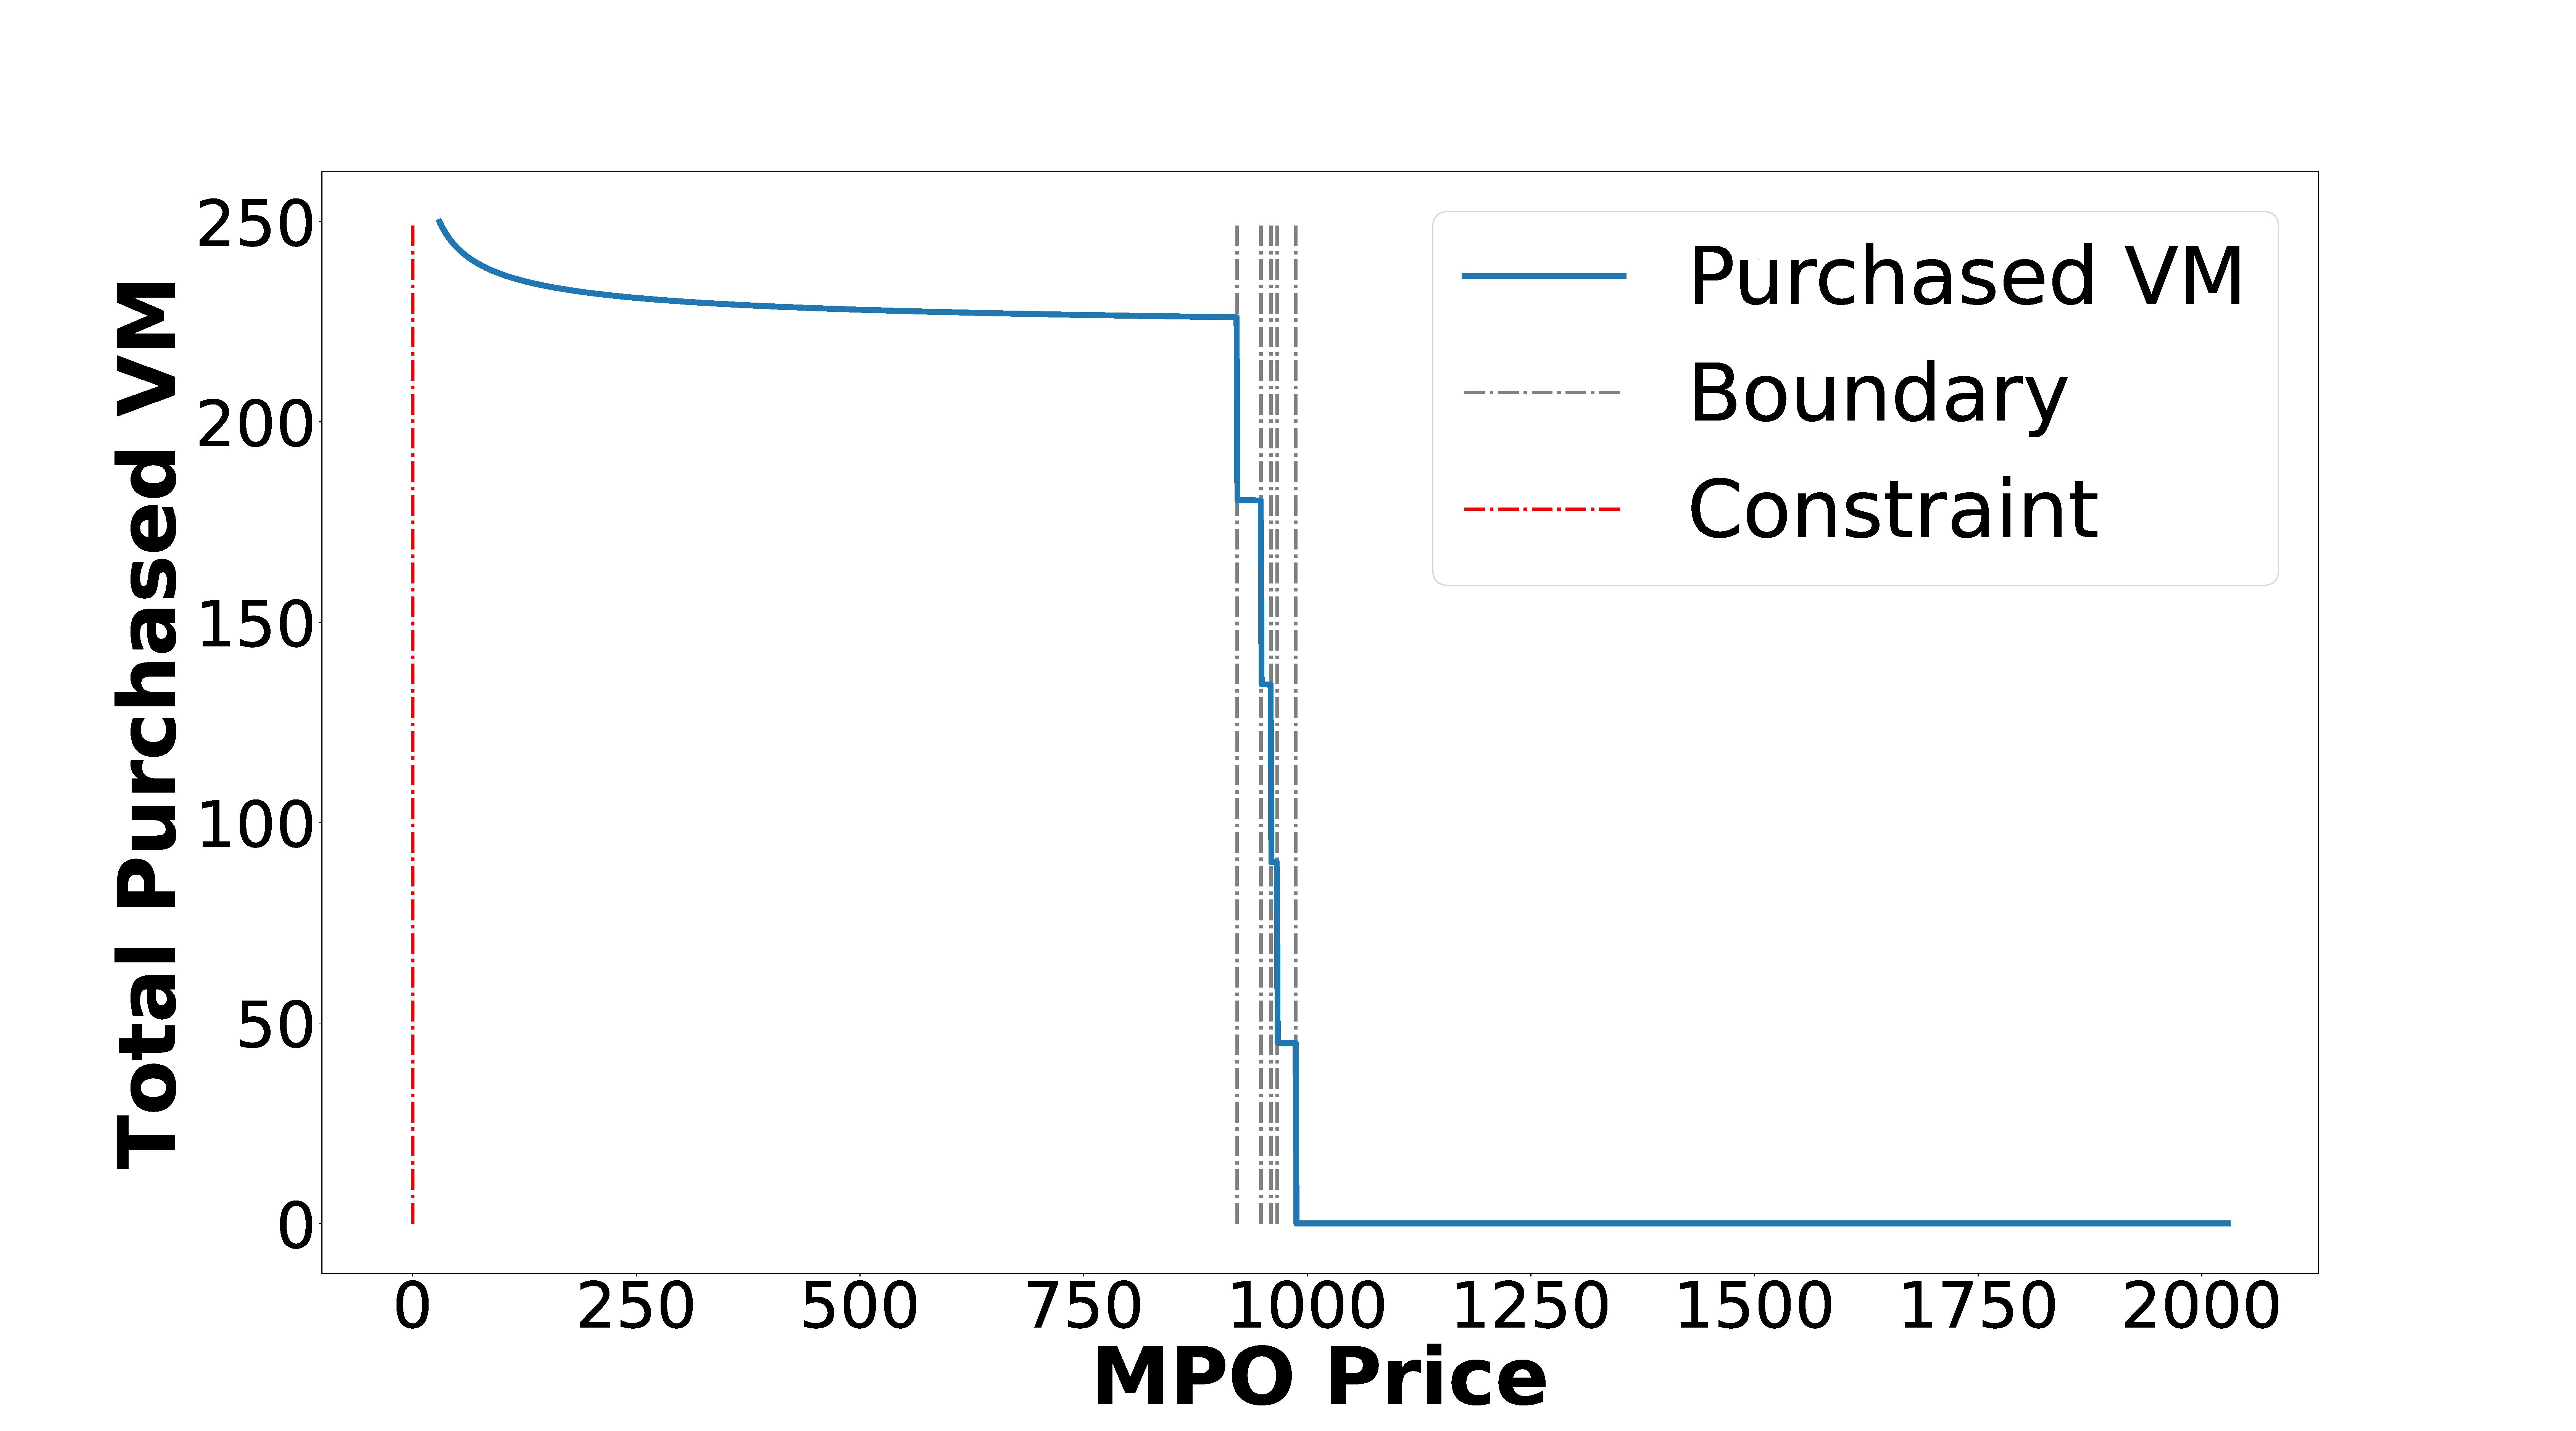
\includegraphics[width=1\textwidth]{5GDDoS_Game_plot_purchased_vm_number.pdf}
        \caption{Total Purchased VM v.s. MPO Price}
        \label{fig:VMnum}
    \end{minipage}
    \begin{minipage}{0.45\linewidth}
        \centering
        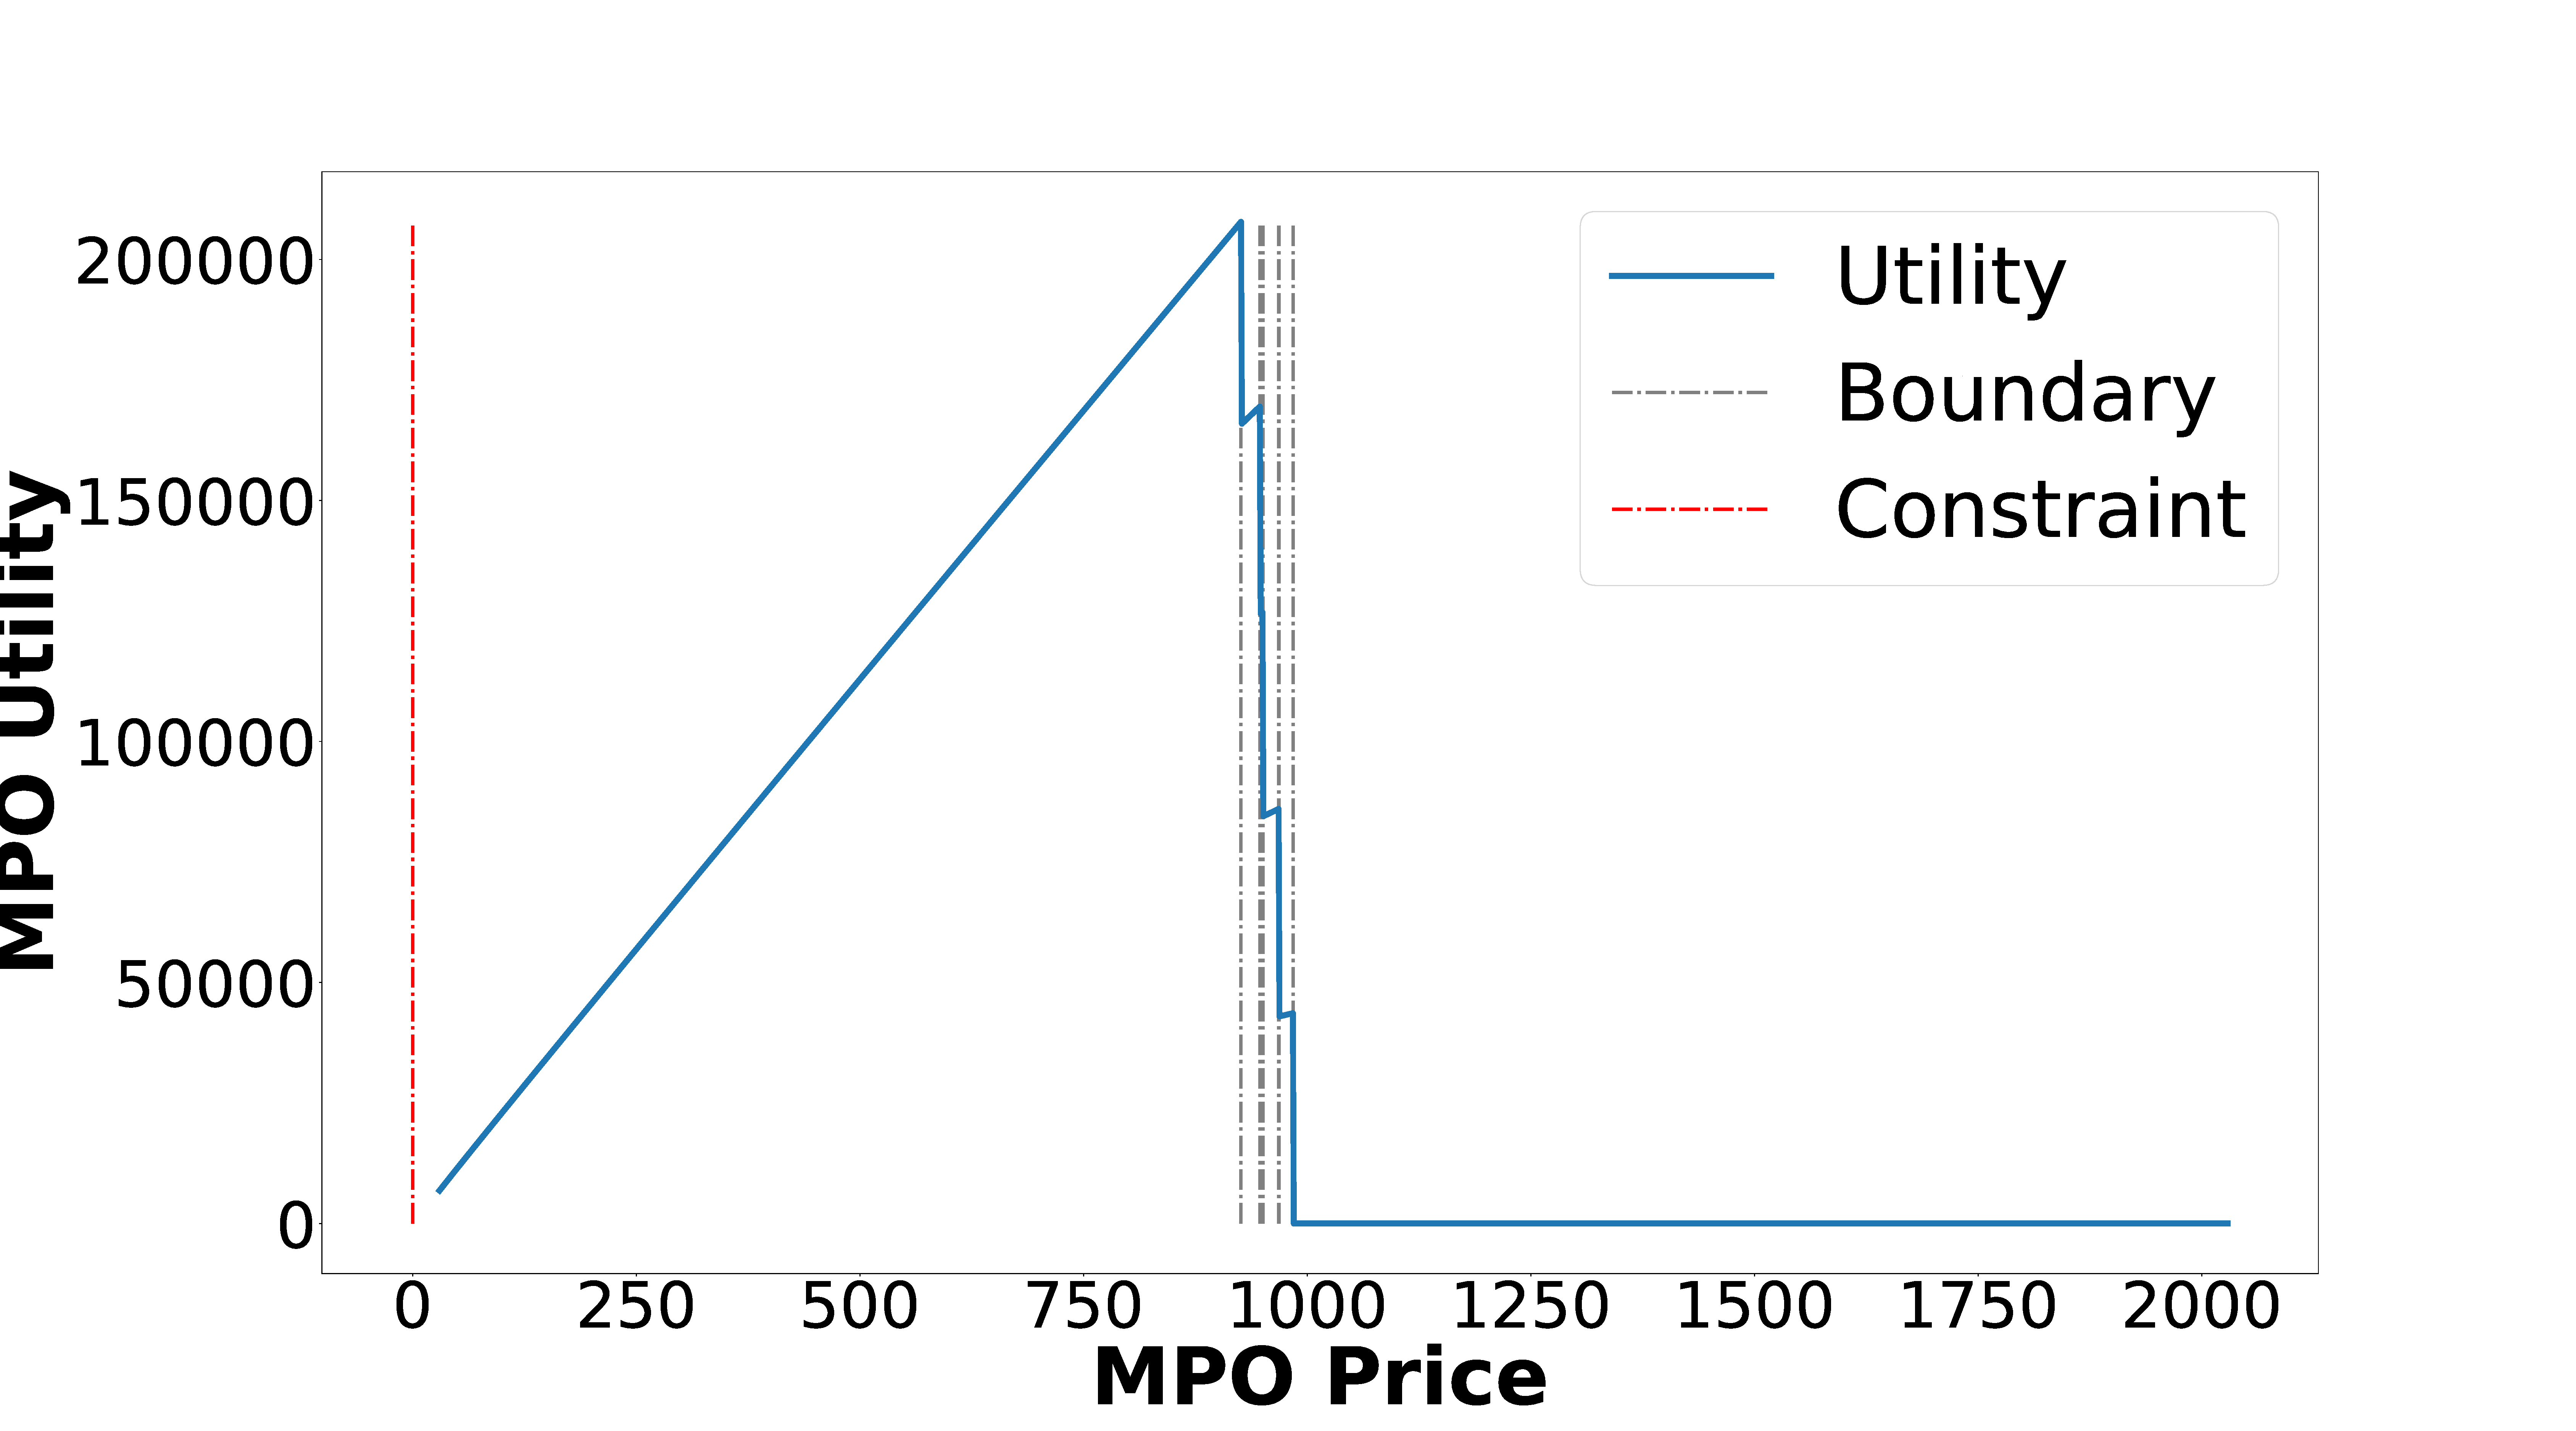
\includegraphics[width=1\textwidth]{5GDDoS_Game_plot_MPO_utility.pdf}
        \caption{MPO Utility v.s. MPO Price}
        \label{fig:MPOutil}
    \end{minipage}
\end{figure}

\subsection{Comparison between various number of EUs}
In this section, we compare multiple IPS VM deployment schemes on ASPs with various numbers of EUs. We consider two cases: ASP with high workload EUs and ASP with low workload EUs. In ASP with high and low workload EUs, the task size $s_{ij}$ is chosen uniformly between $11 - 12$ kB and $8 - 9$ kB, respectively. We discuss the results under these two types of ASP in the following. 
\begin{figure*}[!]
\captionsetup{justification=centering}
  \subfloat[Social Welfare\label{fig:num_cmp_soc_high}]{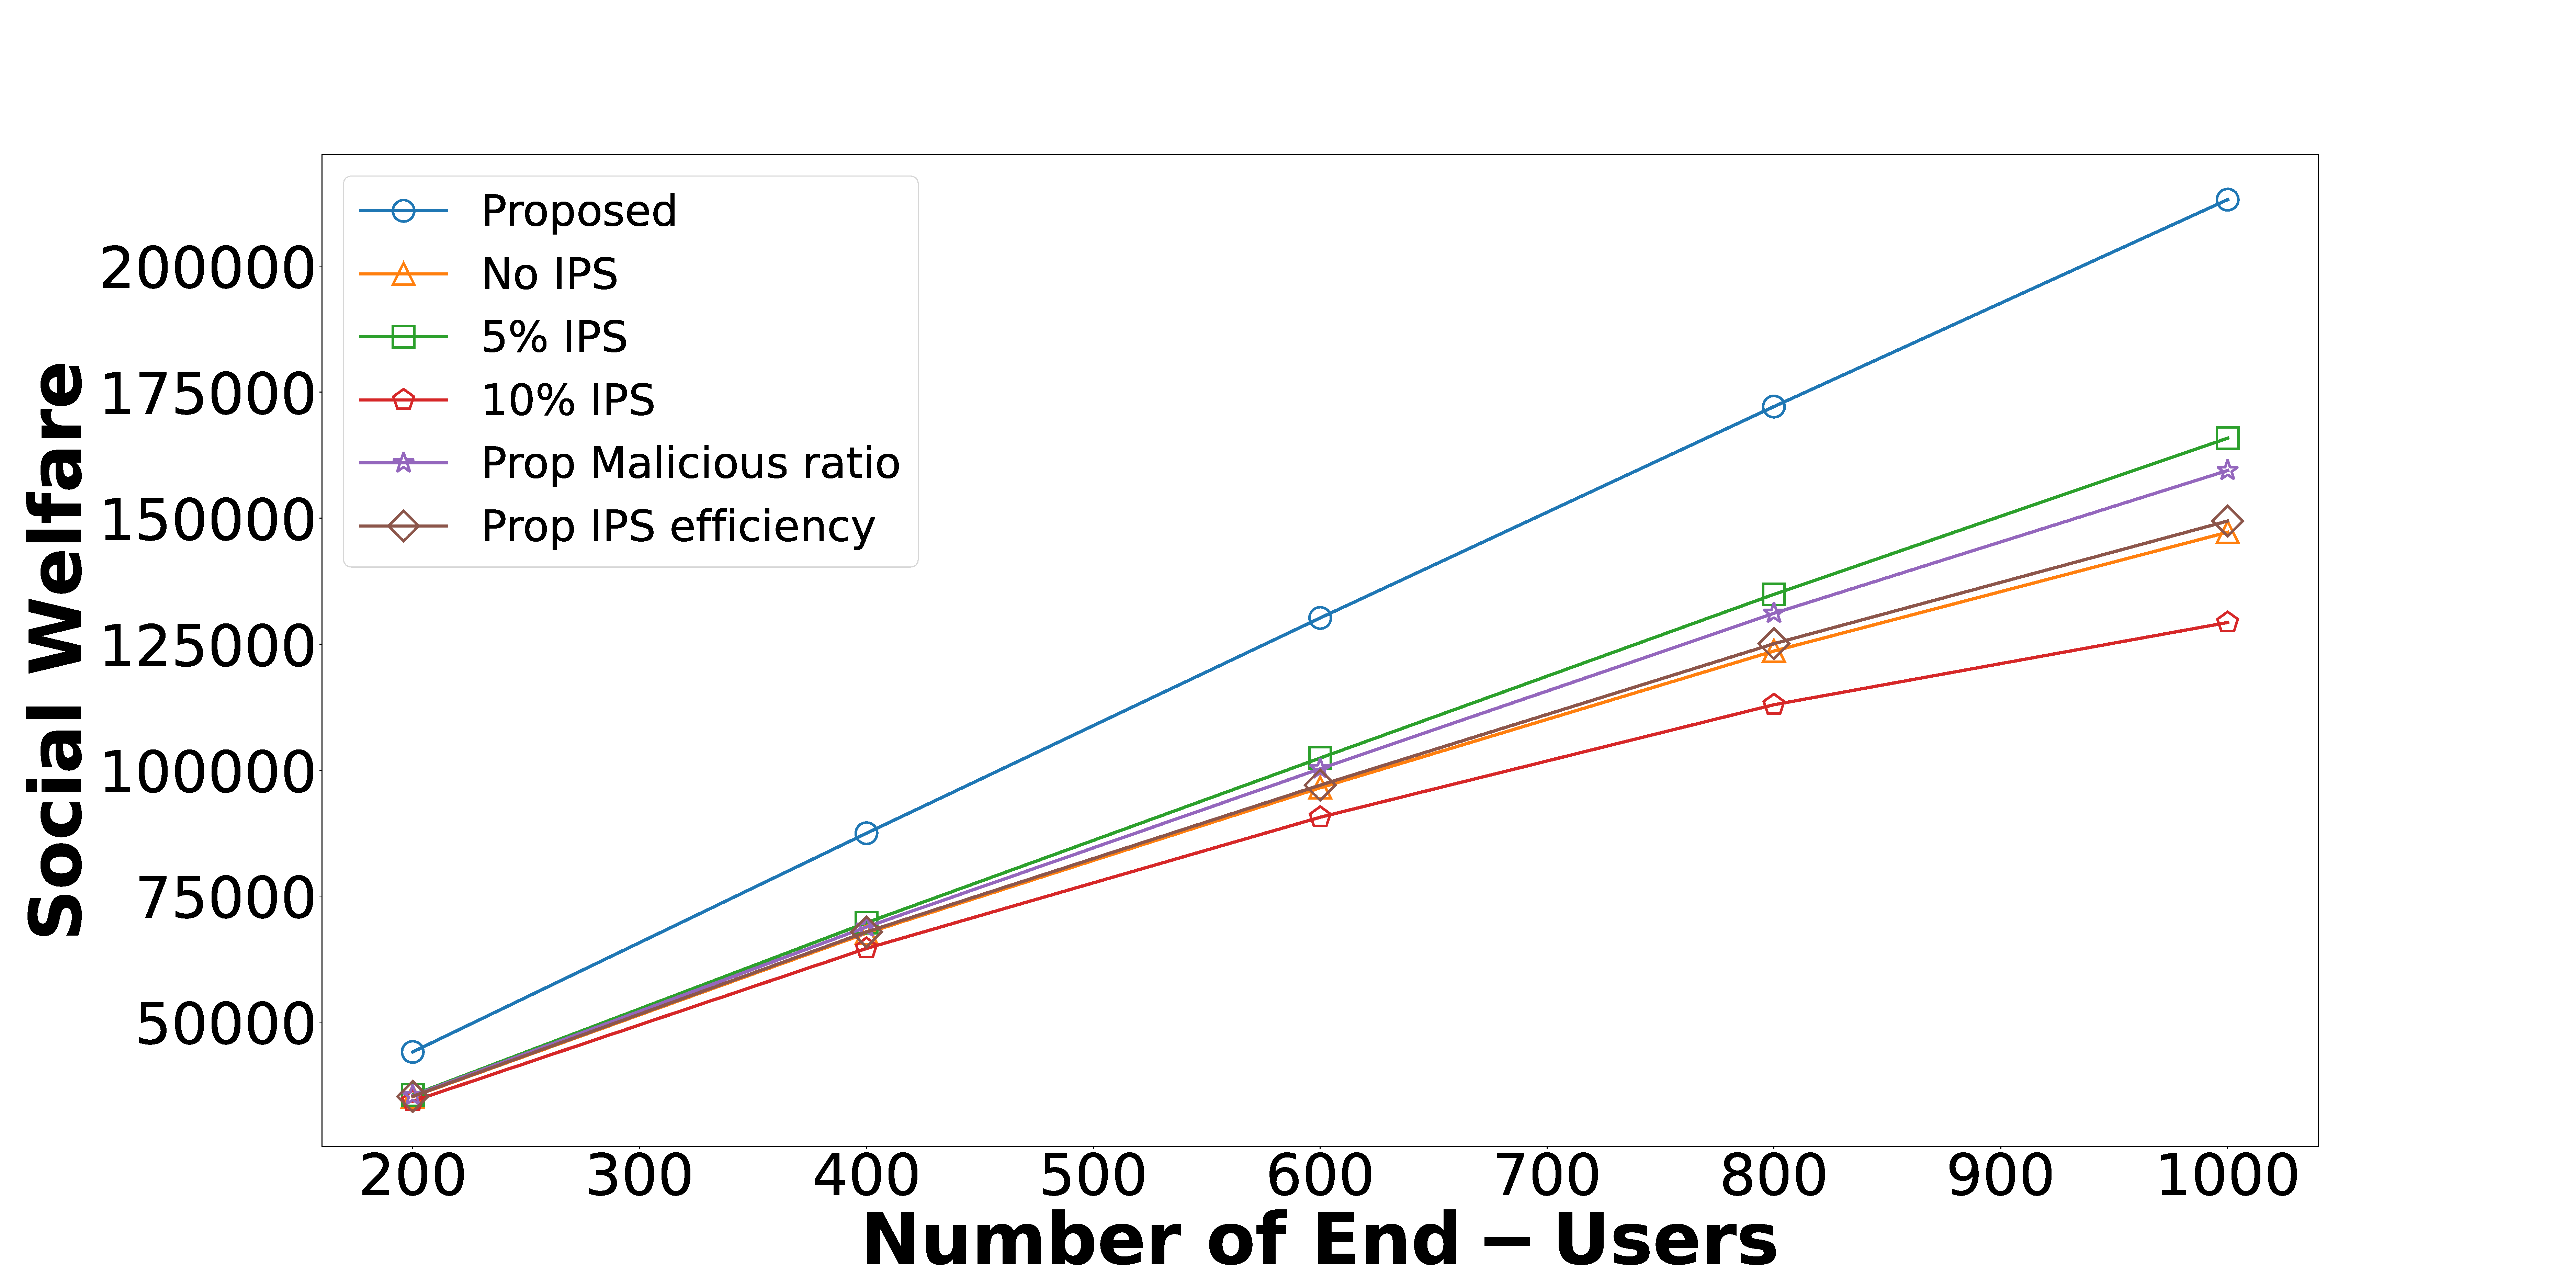
\includegraphics[width=0.33\textwidth]{5GDDoS_Game_social_device_high_cvx.pdf}}
  \hfill
  \subfloat[ASP Utility\label{fig:num_cmp_asp_high}]{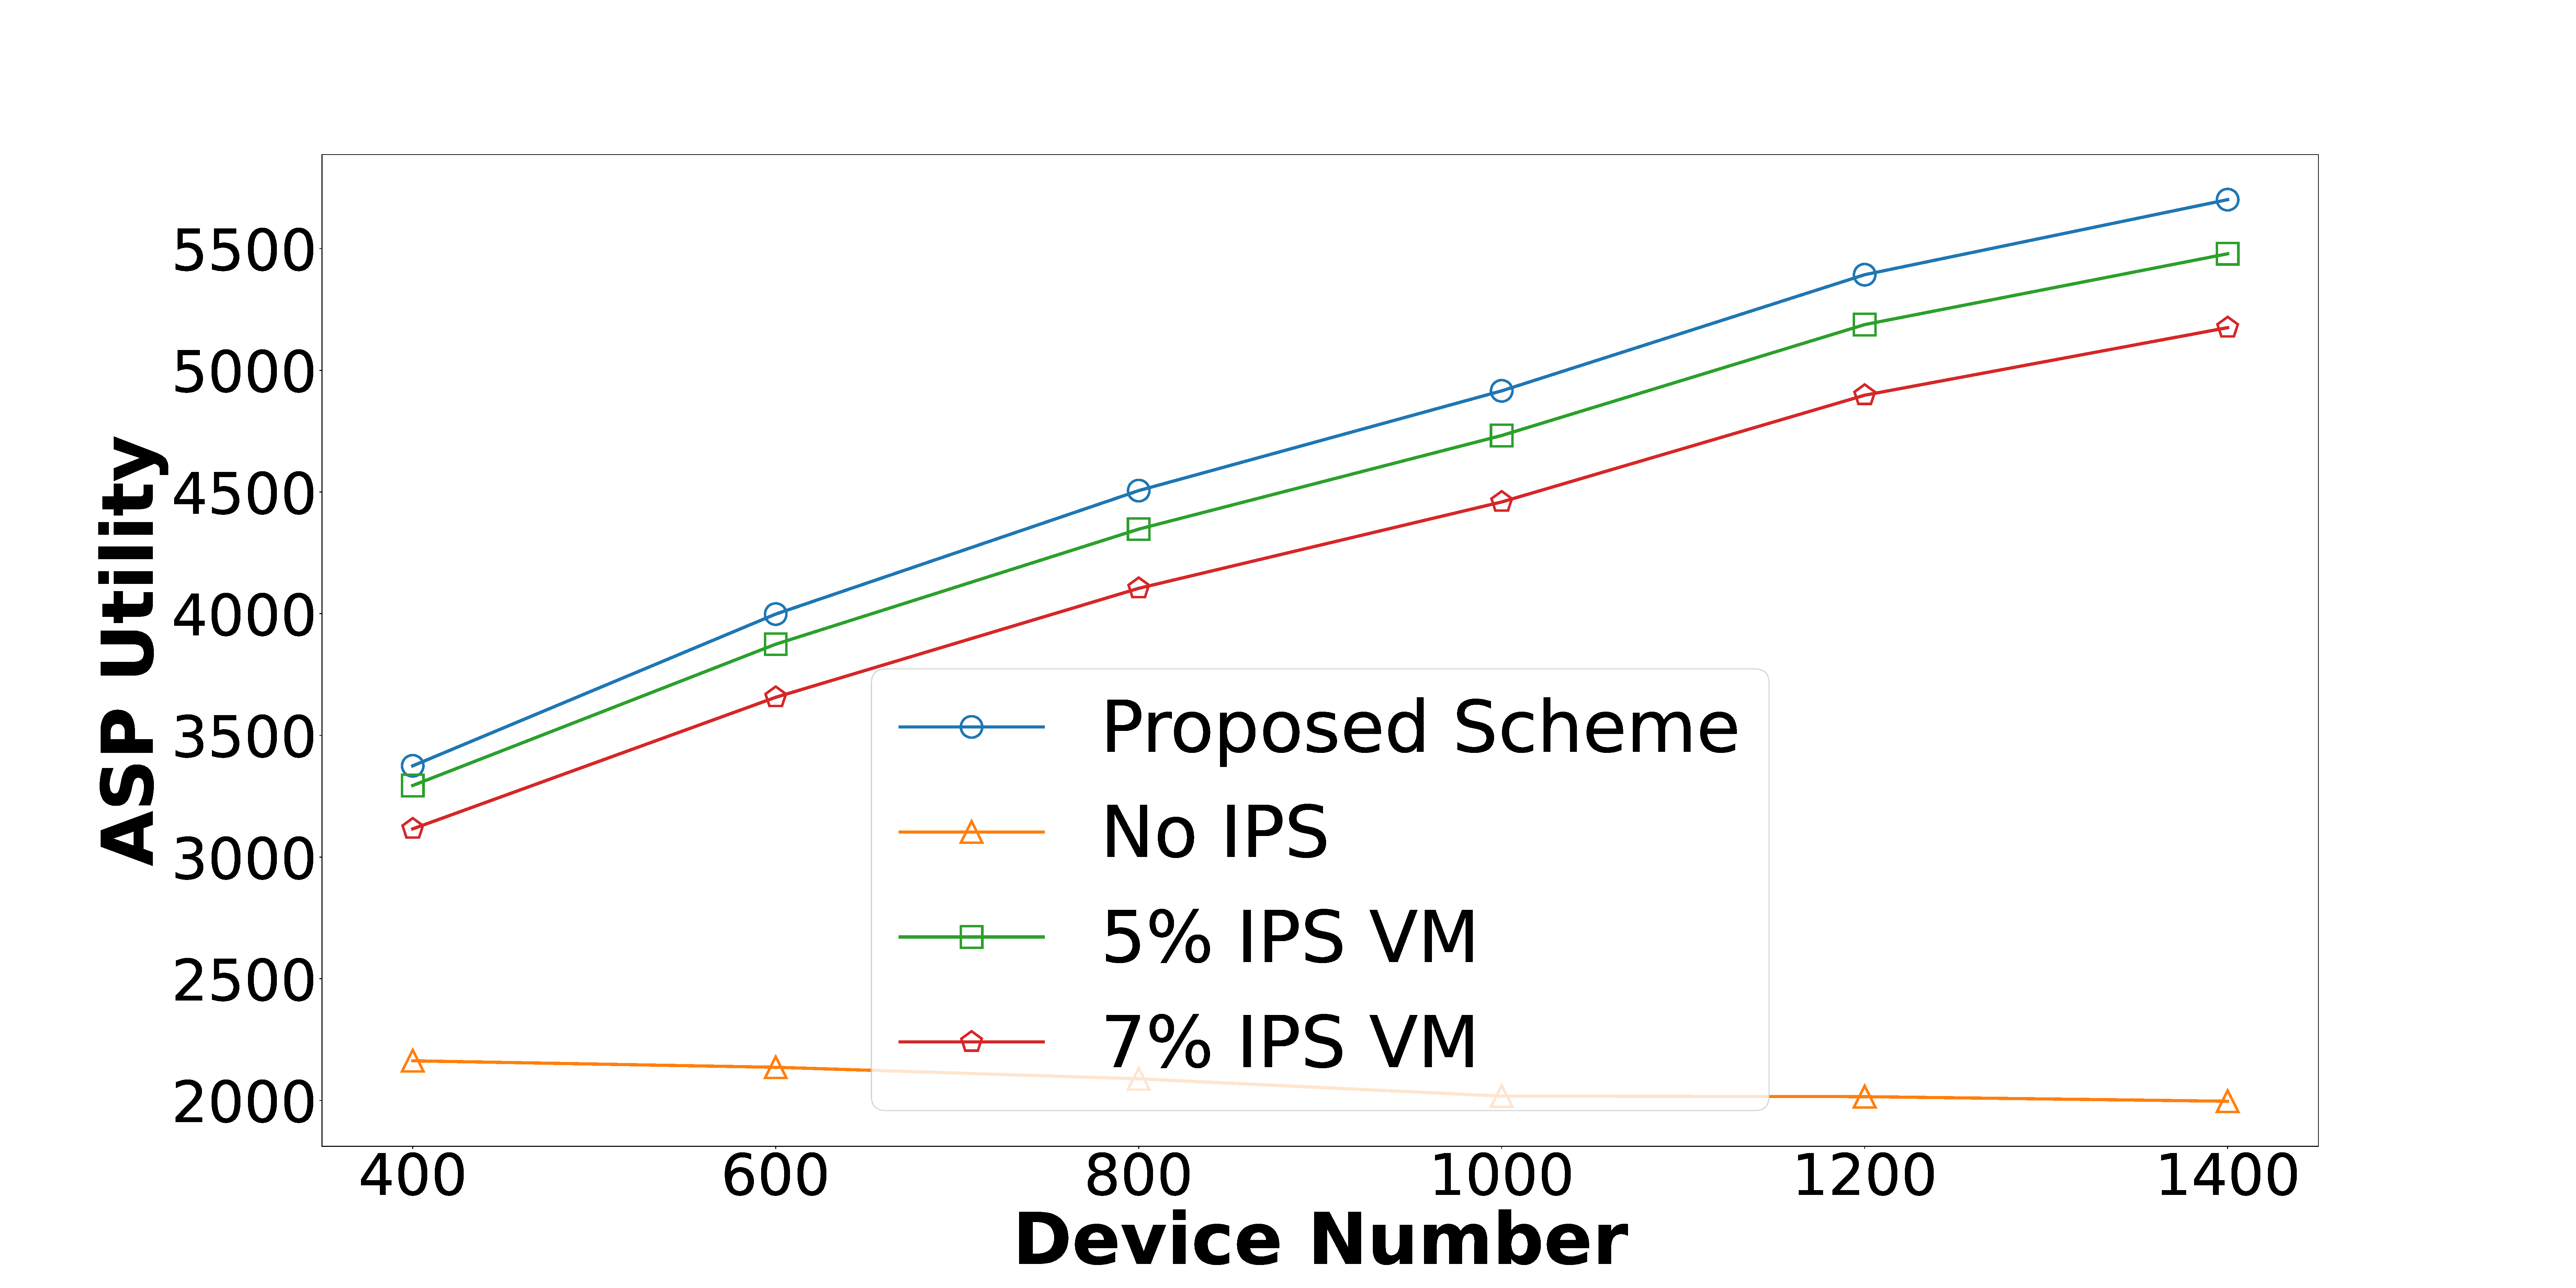
\includegraphics[width=0.33\textwidth] {5GDDoS_Game_asp_device_high_cvx.pdf}}
  \hfill
  \subfloat[MPO Utility\label{fig:num_cmp_mpo_high}]{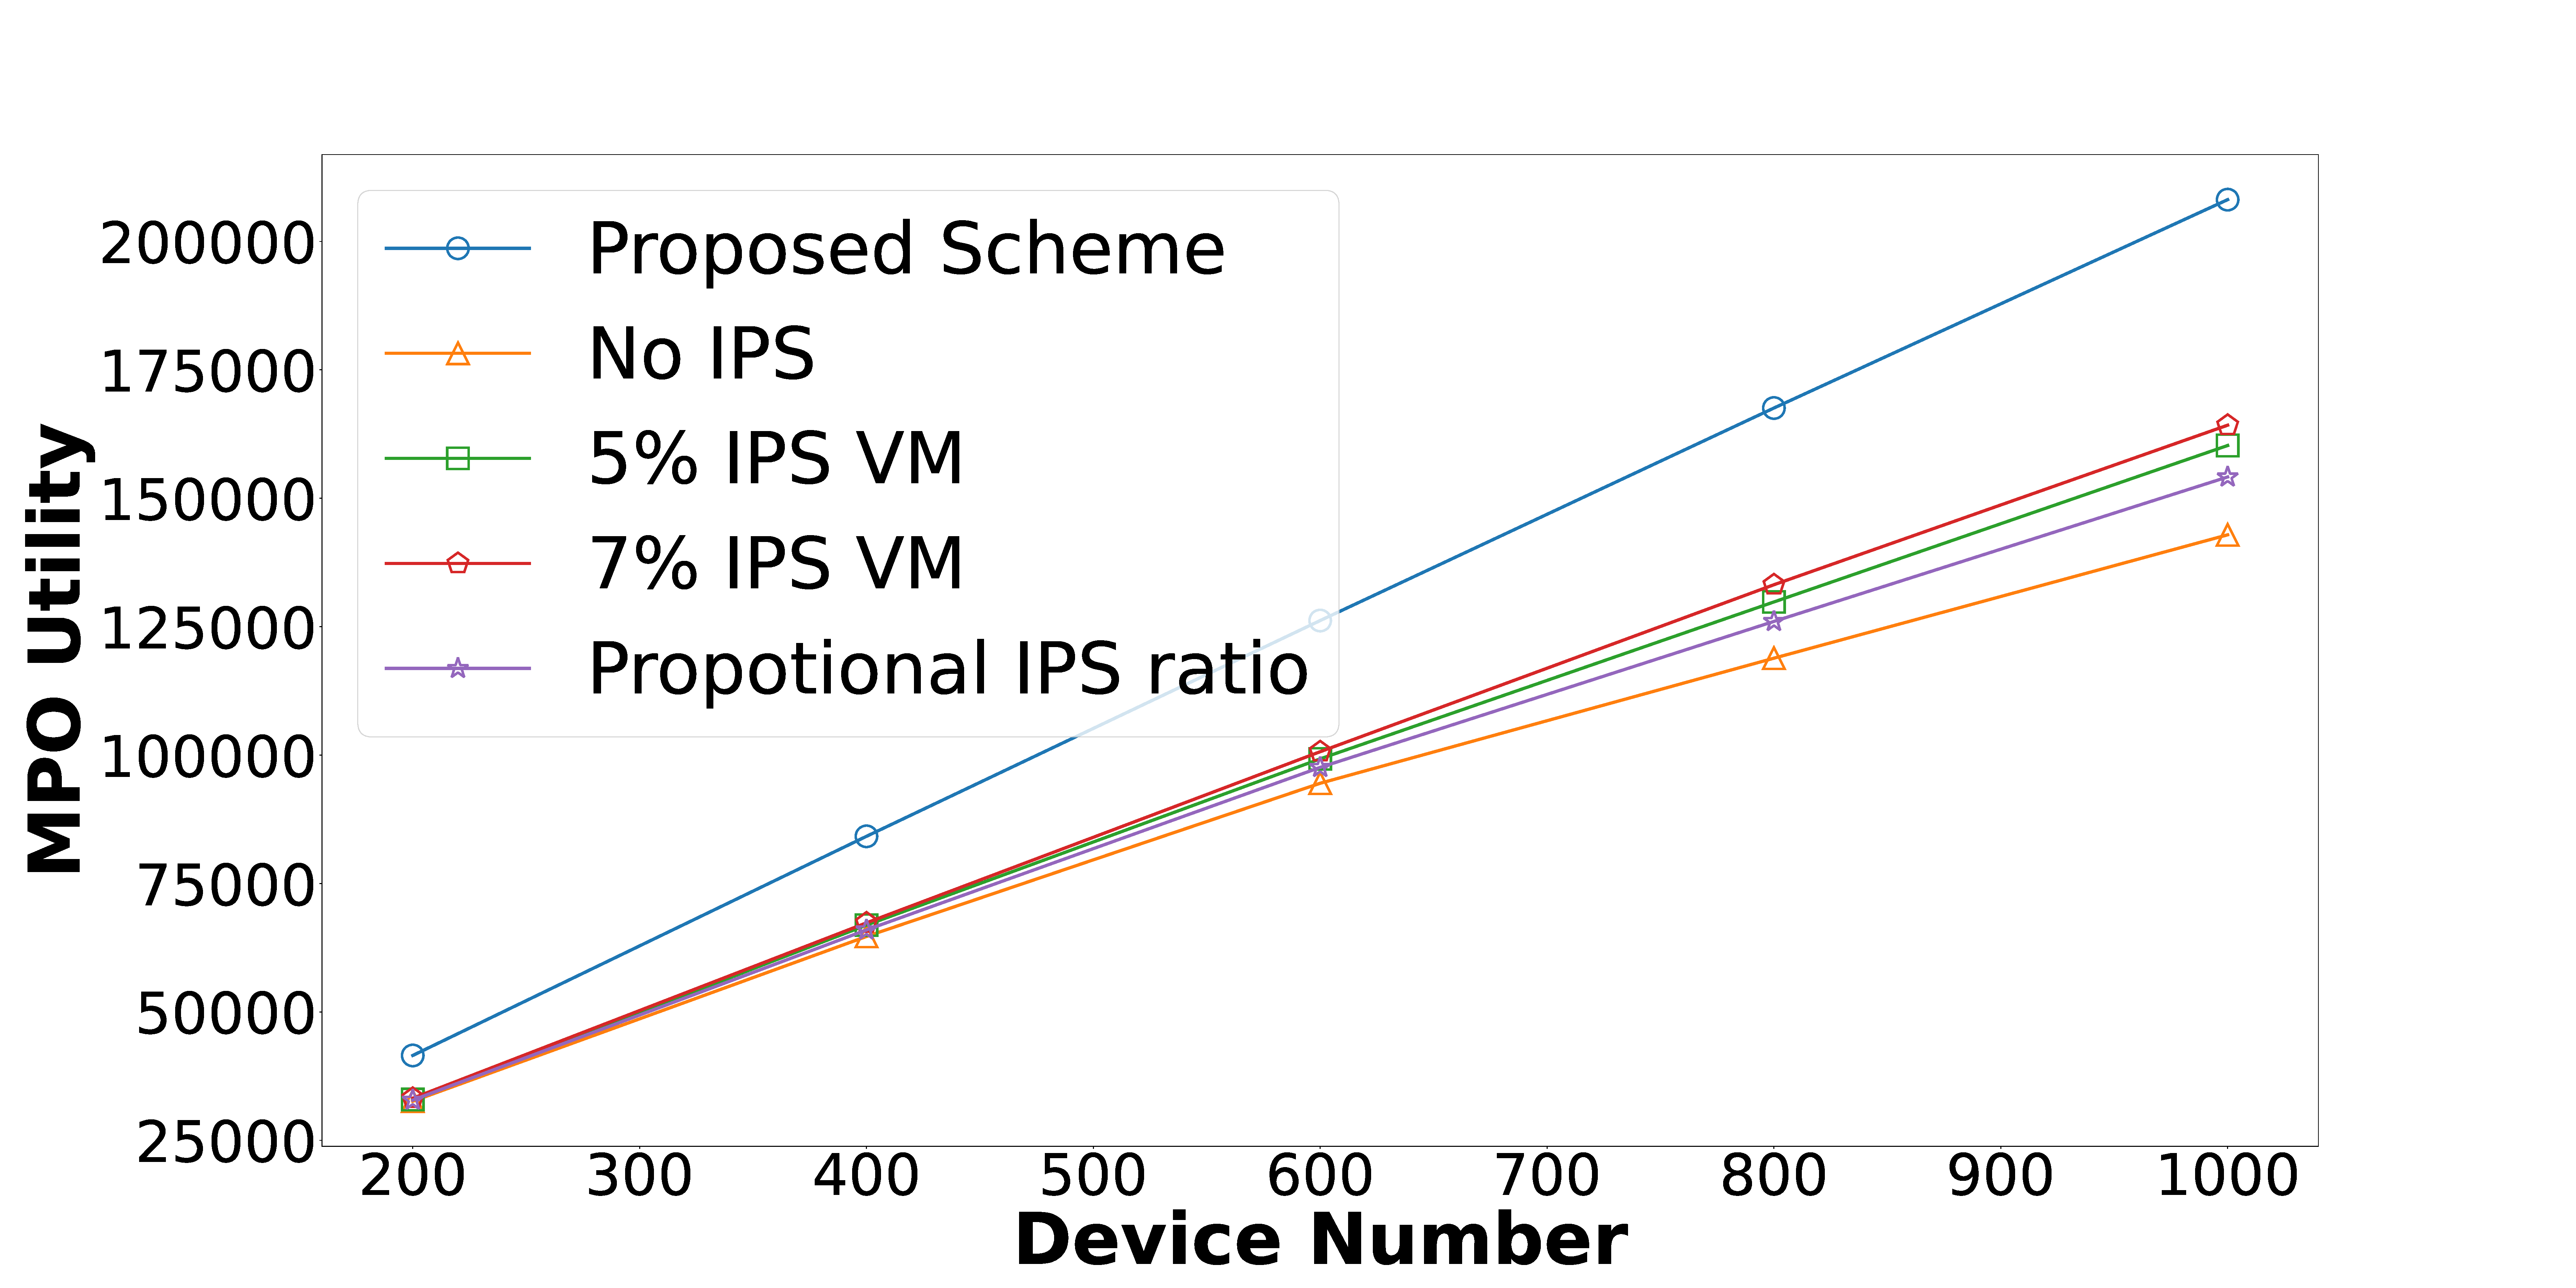
\includegraphics[width=0.33\textwidth]{5GDDoS_Game_MPO_device_high_cvx.pdf}}
\label{fig:num_cmp_high}
\caption{Different Number of High Workload EUs}
\end{figure*}

\textbf{ASP with high workload EUs}: 
When considering ASP with high workload EUs, by (\ref{eqn:service_rate}), we find out that because the required CPU cycles are higher, the service rate is lower than the low workload case. In this simulation, the service rate is lower than the interception rate of IPS VMs. Thus, the ASP has the incentive to deploy VMs on IPS services as possible to eradicate malicious requests. In \Cref{fig:num_cmp_asp_high}, the \textit{7\% IPS VM} scheme has better utility than \textit{5\% IPS VM} scheme because ASP has the incentive to deploy IPS services. Moreover, in \Cref{fig:num_cmp_mpo_high} and \Cref{fig:num_cmp_soc_high} we can discover the same phenomenon. However, \textit{10\% IPS VM} has lower utility due to the deployment of redundant IPS. When the number of users increases, the utility of ASPs starts to increase because they can serve more users, and the utility of MPO increases because the ASPs buy more VMs from the MPO to serve more users, so the total social welfare also increases. In this scenario, both \textit{Proportional malicious ratio} and \textit{Proportional IPS efficiency} allocate fixed ratio of IPS VMs because the ratio of malicious to total users and IPS efficiency are both fixed, which is $30 * 0.1 = 3\%$ and $0.01 * 50 = 0.5\%$, respectively. Therefore, the utility curves of both schemes in \Cref{fig:num_cmp_asp_high} are similar to the fixed IPS scheme (\textit{5\% IPS VM}, \textit{7\% IPS VM}, and \textit{10\% IPS VM}). In addition, our \textit{Proposed Scheme} has outperformed other schemes in \Cref{fig:num_cmp_soc_high}, \Cref{fig:num_cmp_asp_high}, and \Cref{fig:num_cmp_mpo_high}.

% device num low
\begin{figure*}[!]
\captionsetup{justification=centering}
  \subfloat[Social Welfare\label{fig:num_cmp_soc_low}]{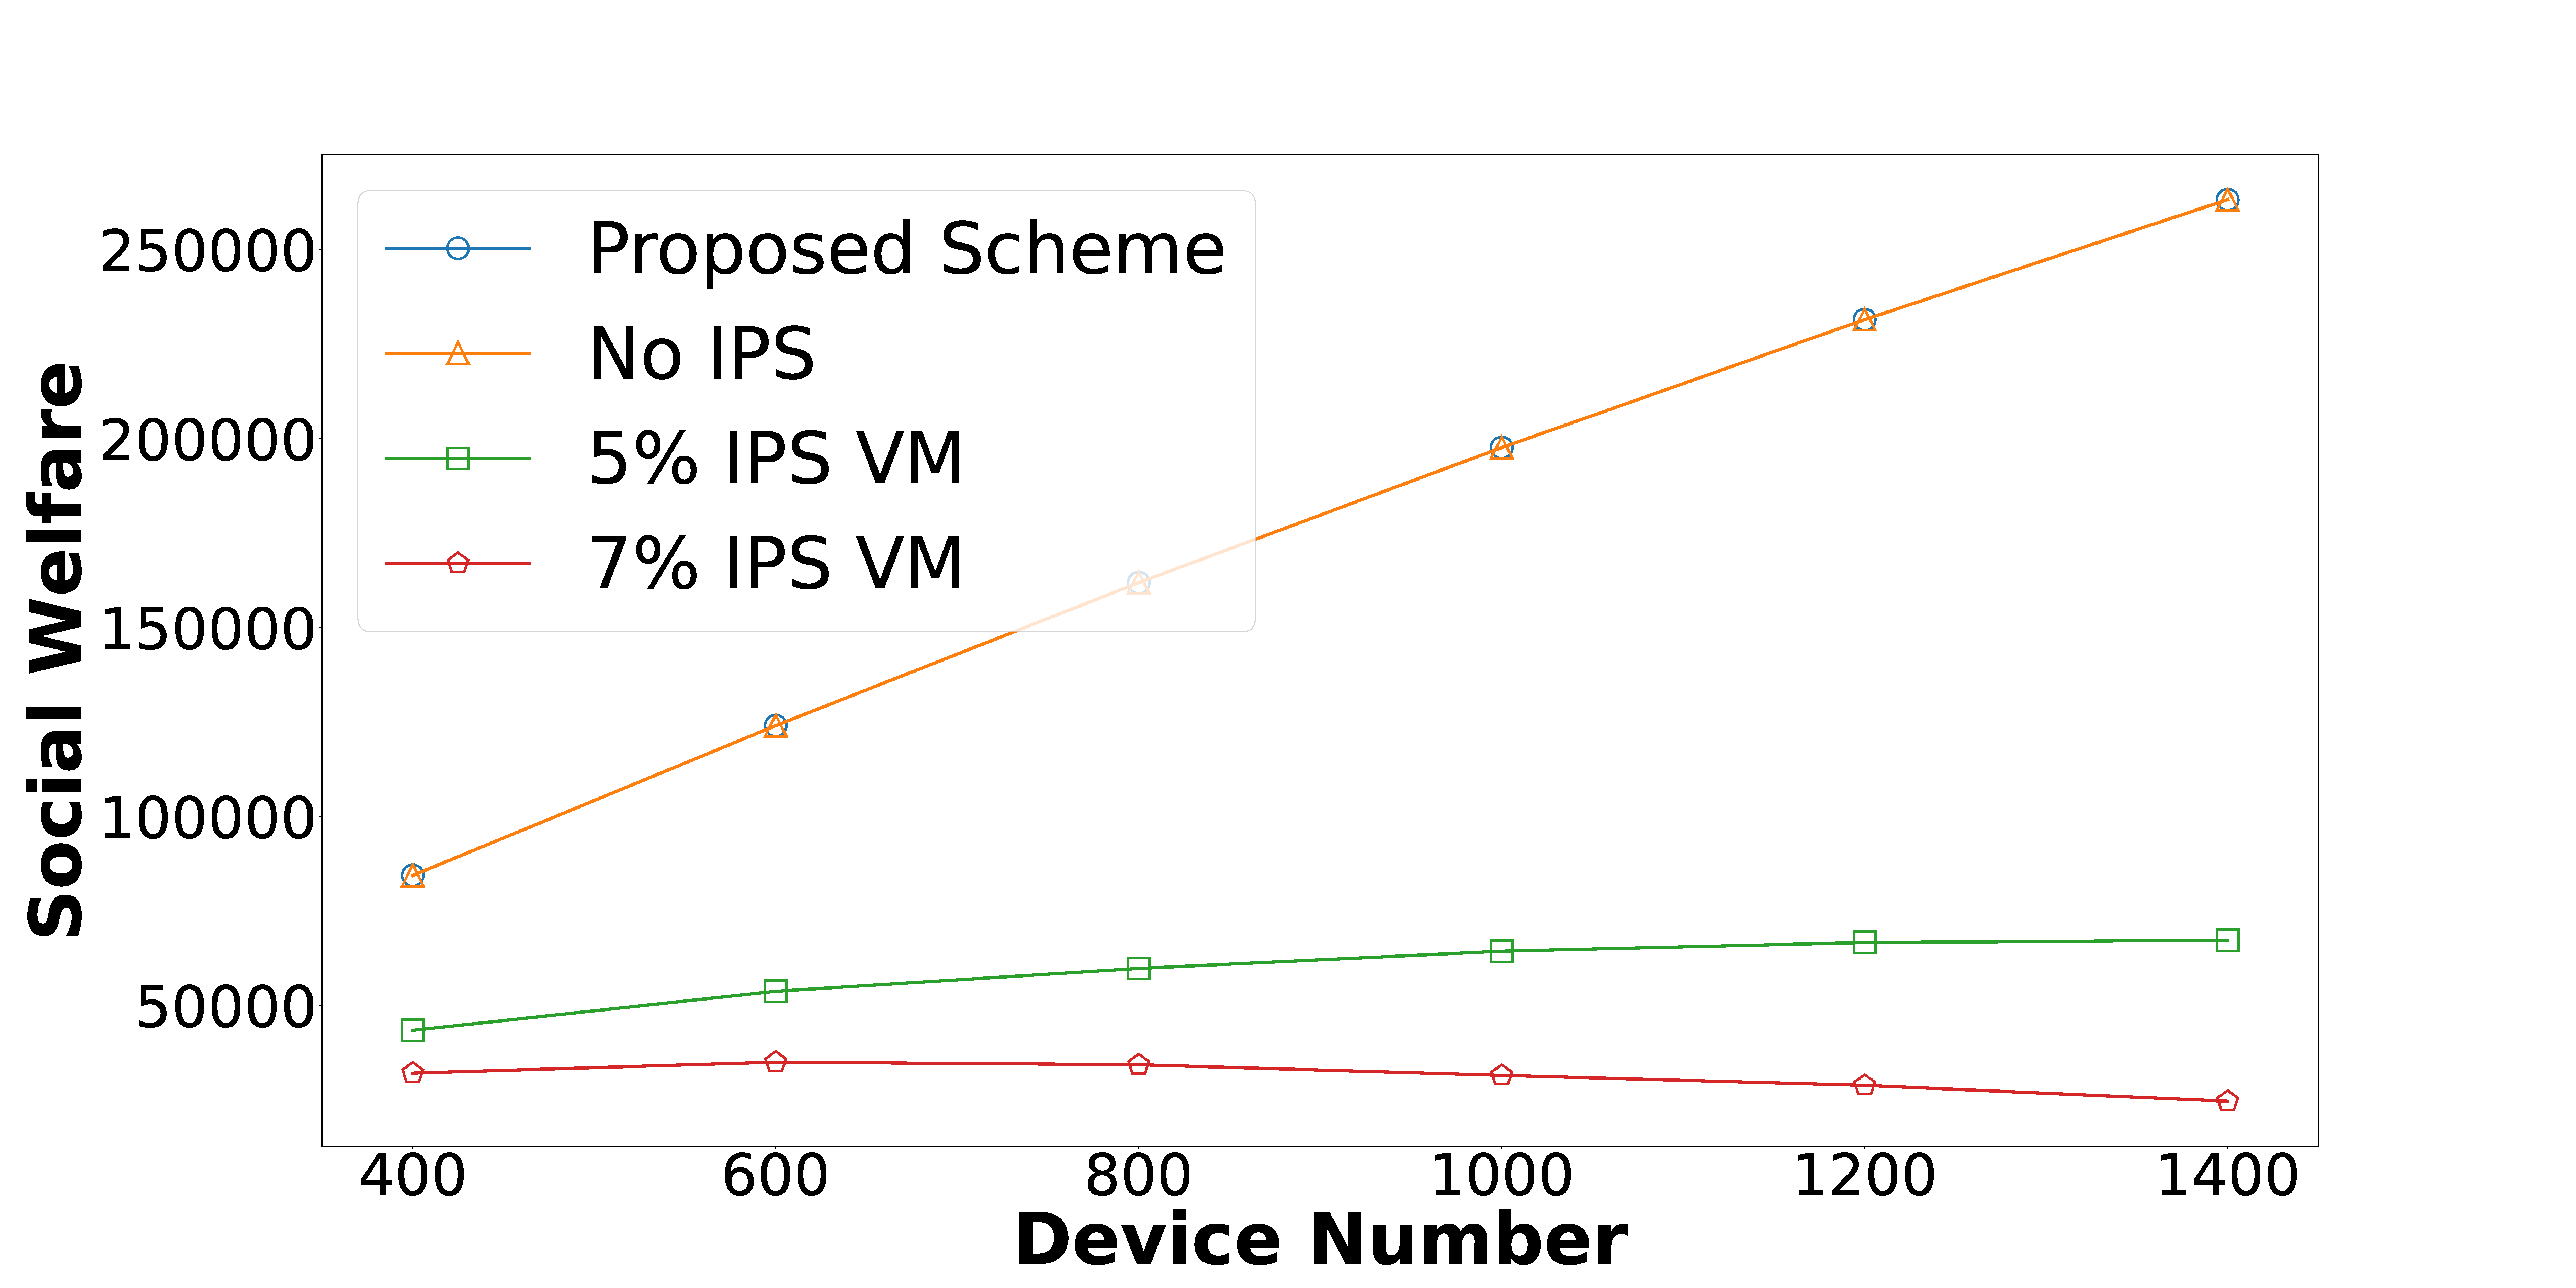
\includegraphics[width=0.33\textwidth]{5GDDoS_Game_social_device_low_cvx.pdf}}
  \hfill
  \subfloat[ASP Utility\label{fig:num_cmp_asp_low}]{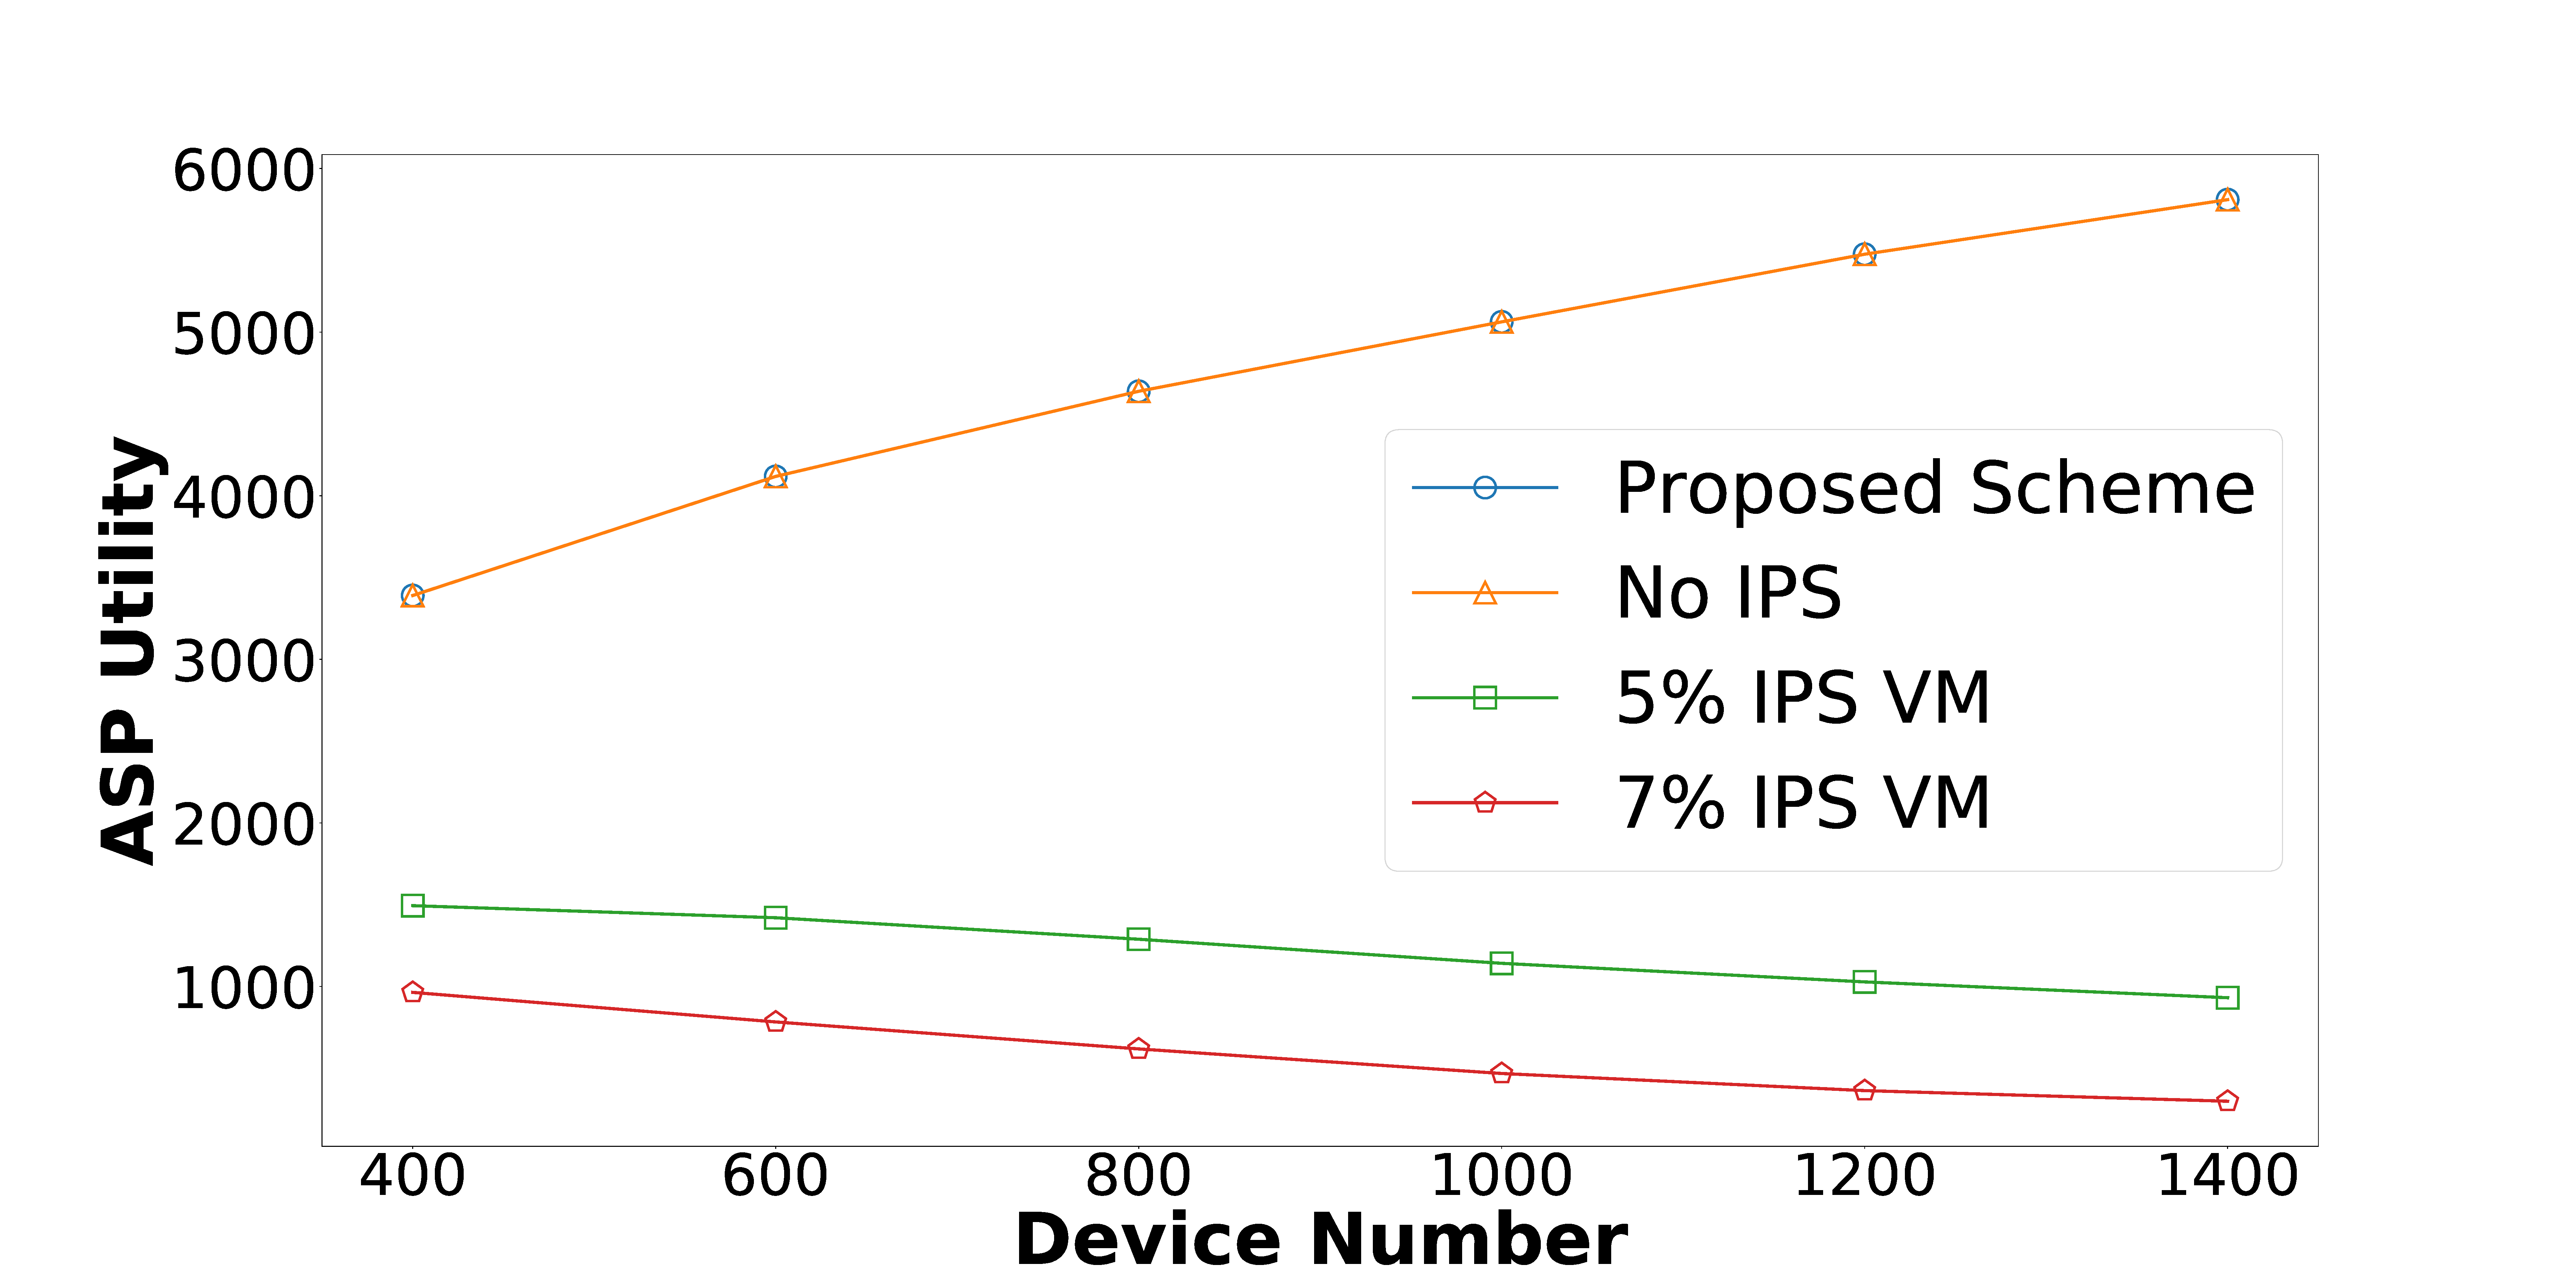
\includegraphics[width=0.33\textwidth] {5GDDoS_Game_asp_device_low_cvx.pdf}}
  \hfill
  \subfloat[MPO Utility\label{fig:num_cmp_mpo_low}]{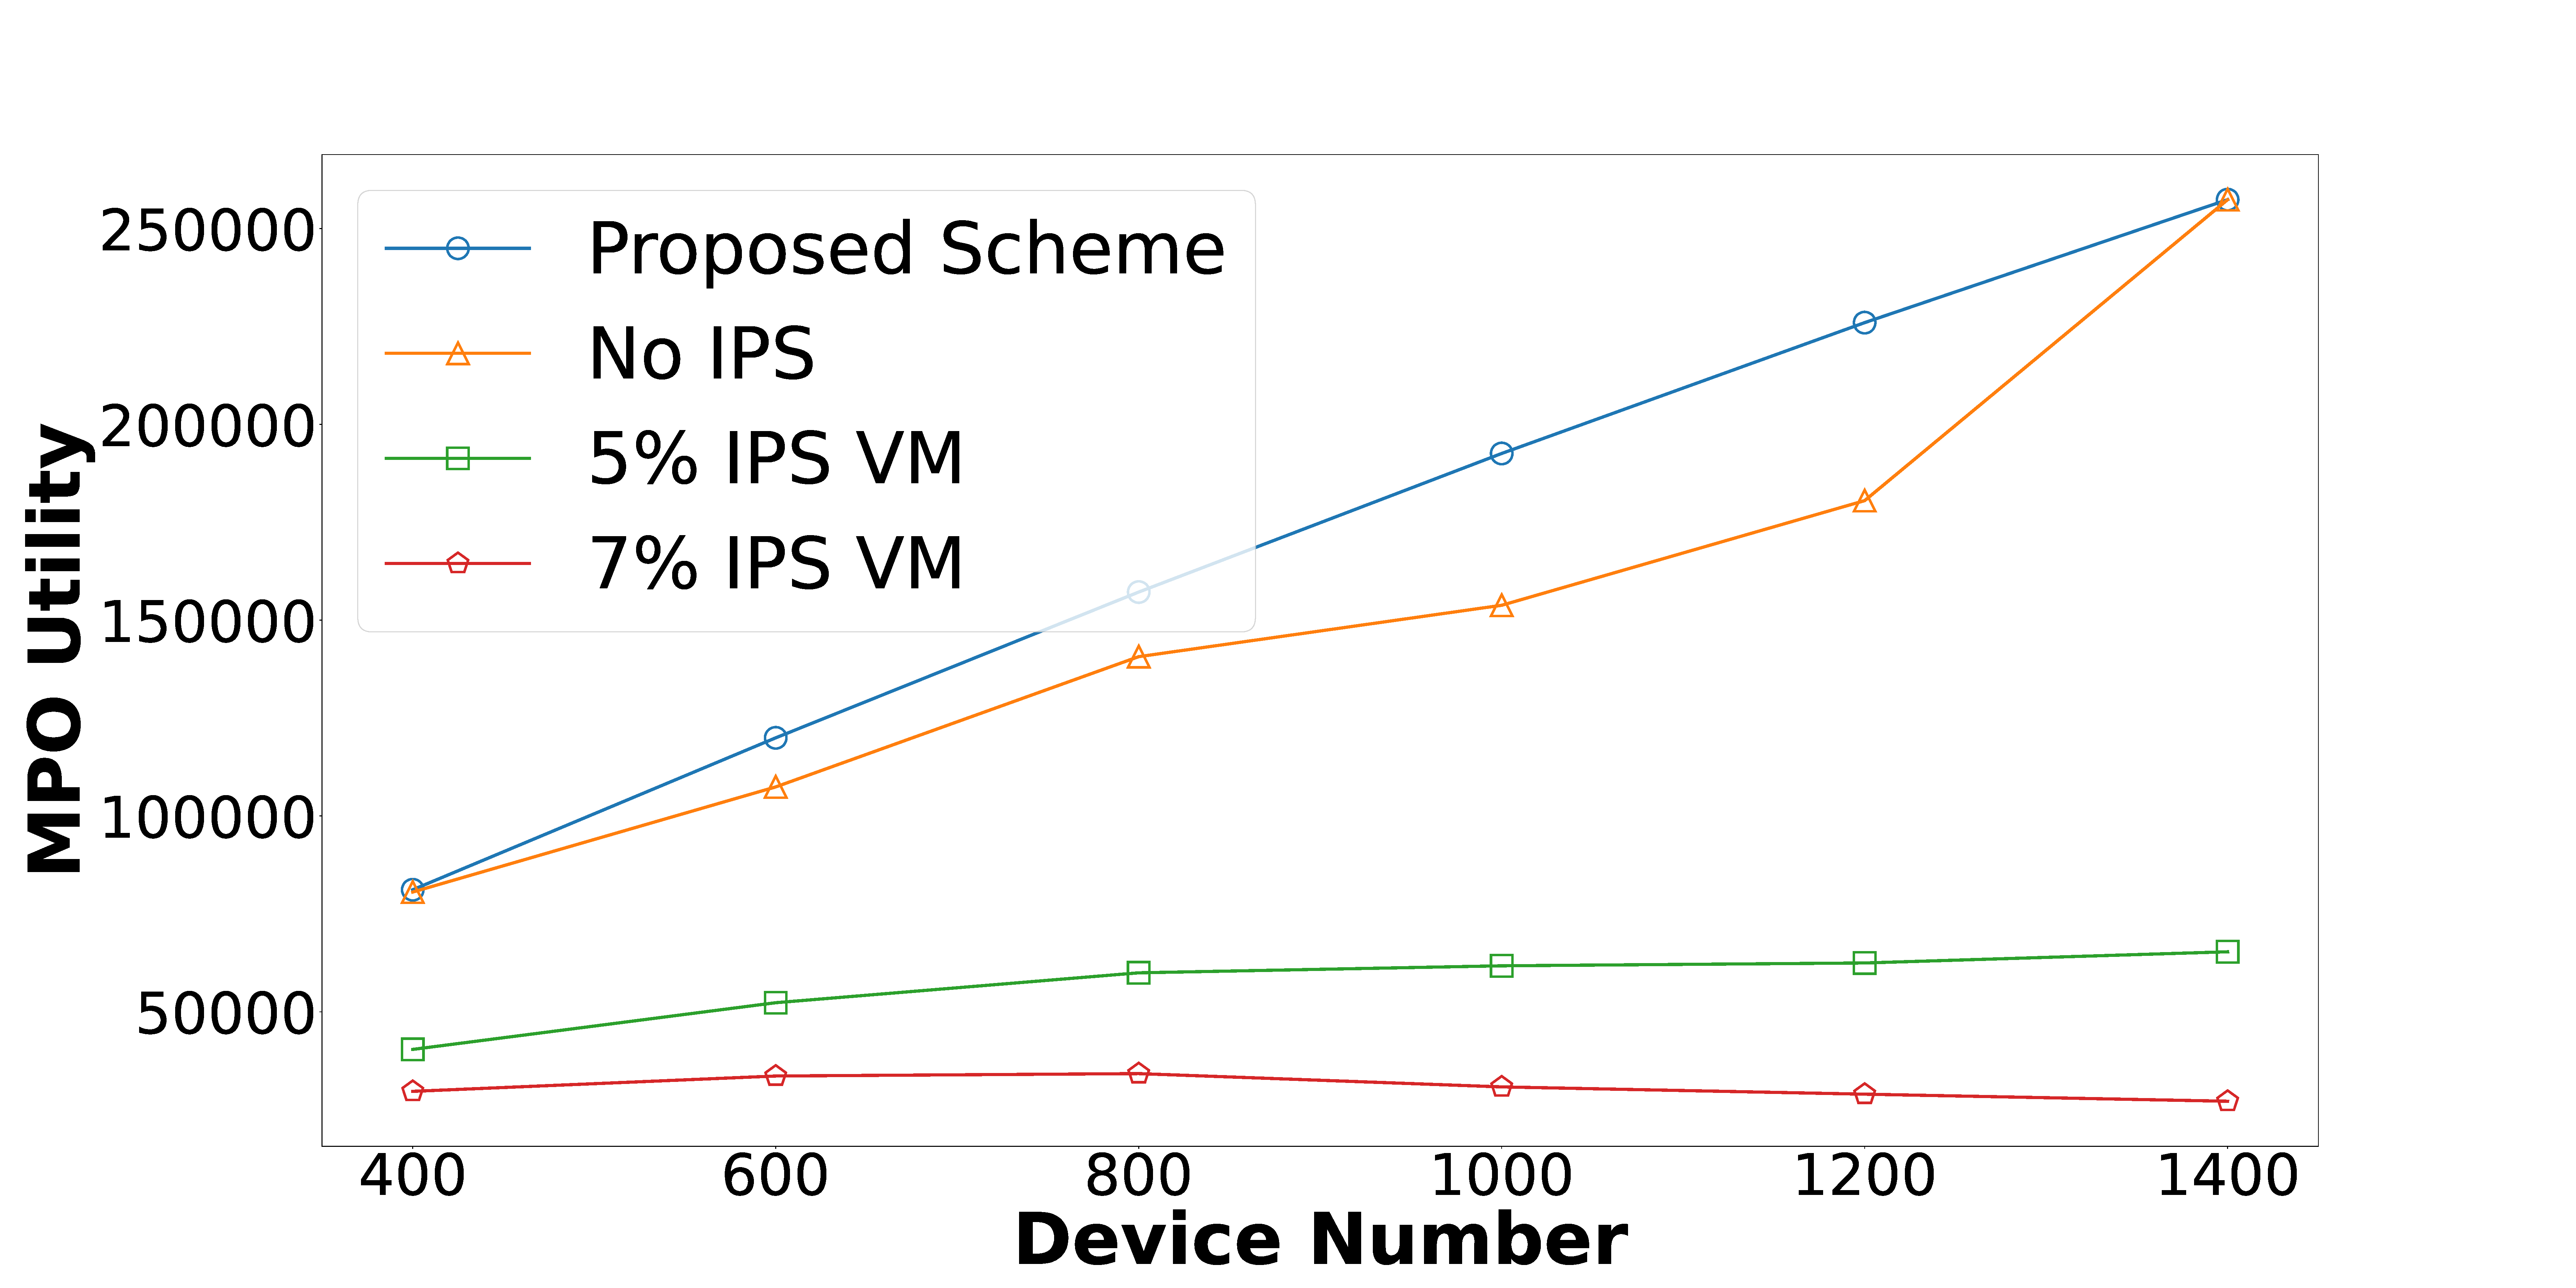
\includegraphics[width=0.33\textwidth]{5GDDoS_Game_MPO_device_low_cvx.pdf}}
\label{fig:num_cmp_low}
\caption{Different Number of Low Workload EUs}
\end{figure*}

\textbf{ASP with low workload EUs}:
Considering ASP with low workload EUs, the required CPU cycles are low. Different from the high-workload case, in this case, the service rate is higher than the interception rate of IPS VMs, and the ASP has more incentive to deploy VMs to serve EUs than to wipe out malicious requests. Therefore, the optimal deployment scheme for such ASPs is identical to the \textit{No IPS} scheme. We can observe the phenomenon in \Cref{fig:num_cmp_asp_low}. Moreover, the ASPs' utility in \textit{5\% IPS VM} \textit{7\% IPS VM}, and \textit{10\% IPS VM} are lower because it is less efficient for ASPs to deploy IPS VMs than to deploy VMs to serve users. Similar to the high-workload case, both schemes \textit{Proportional malicious ratio} and \textit{Proportional IPS efficiency} allocate fixed ratio of IPS VMs. In this scenario, the \textit{Proportional malicious ratio} scheme allocates $30 \times 0.1 = 3\%$ of IPS VMs, and the \textit{Proportional IPS efficiency} scheme allocates $0.01 \times 50 = 0.5\%$ of IPS VMs. As a result, in \Cref{fig:num_cmp_asp_low}, the \textit{Proportional malicious ratio} has lower utility than \textit{Proportional IPS efficiency} because it is less efficient to deploy IPS VMs in this scenario. In addition, our proposed scheme has the highest utility in \Cref{fig:num_cmp_soc_low}, \Cref{fig:num_cmp_asp_low}, and \Cref{fig:num_cmp_mpo_low}.

\subsection{Comparison between various malicious users to total users ratio}\label{subsec:mal}
We compare different IPS VM deployment schemes on ASPs given various malicious users to total users ratios. Similar to the previous simulation, we discuss two different cases: ASP with high workload EUs and ASP with low workload EUs. The parameters of high and low workload EUs are mentioned in the previous simulation. We discuss the different characteristics of these two types of ASPs. 

% ratio high
\begin{figure*}[!]
\captionsetup{justification=centering}
  \subfloat[Social Welfare\label{fig:ratio_soc_high}]{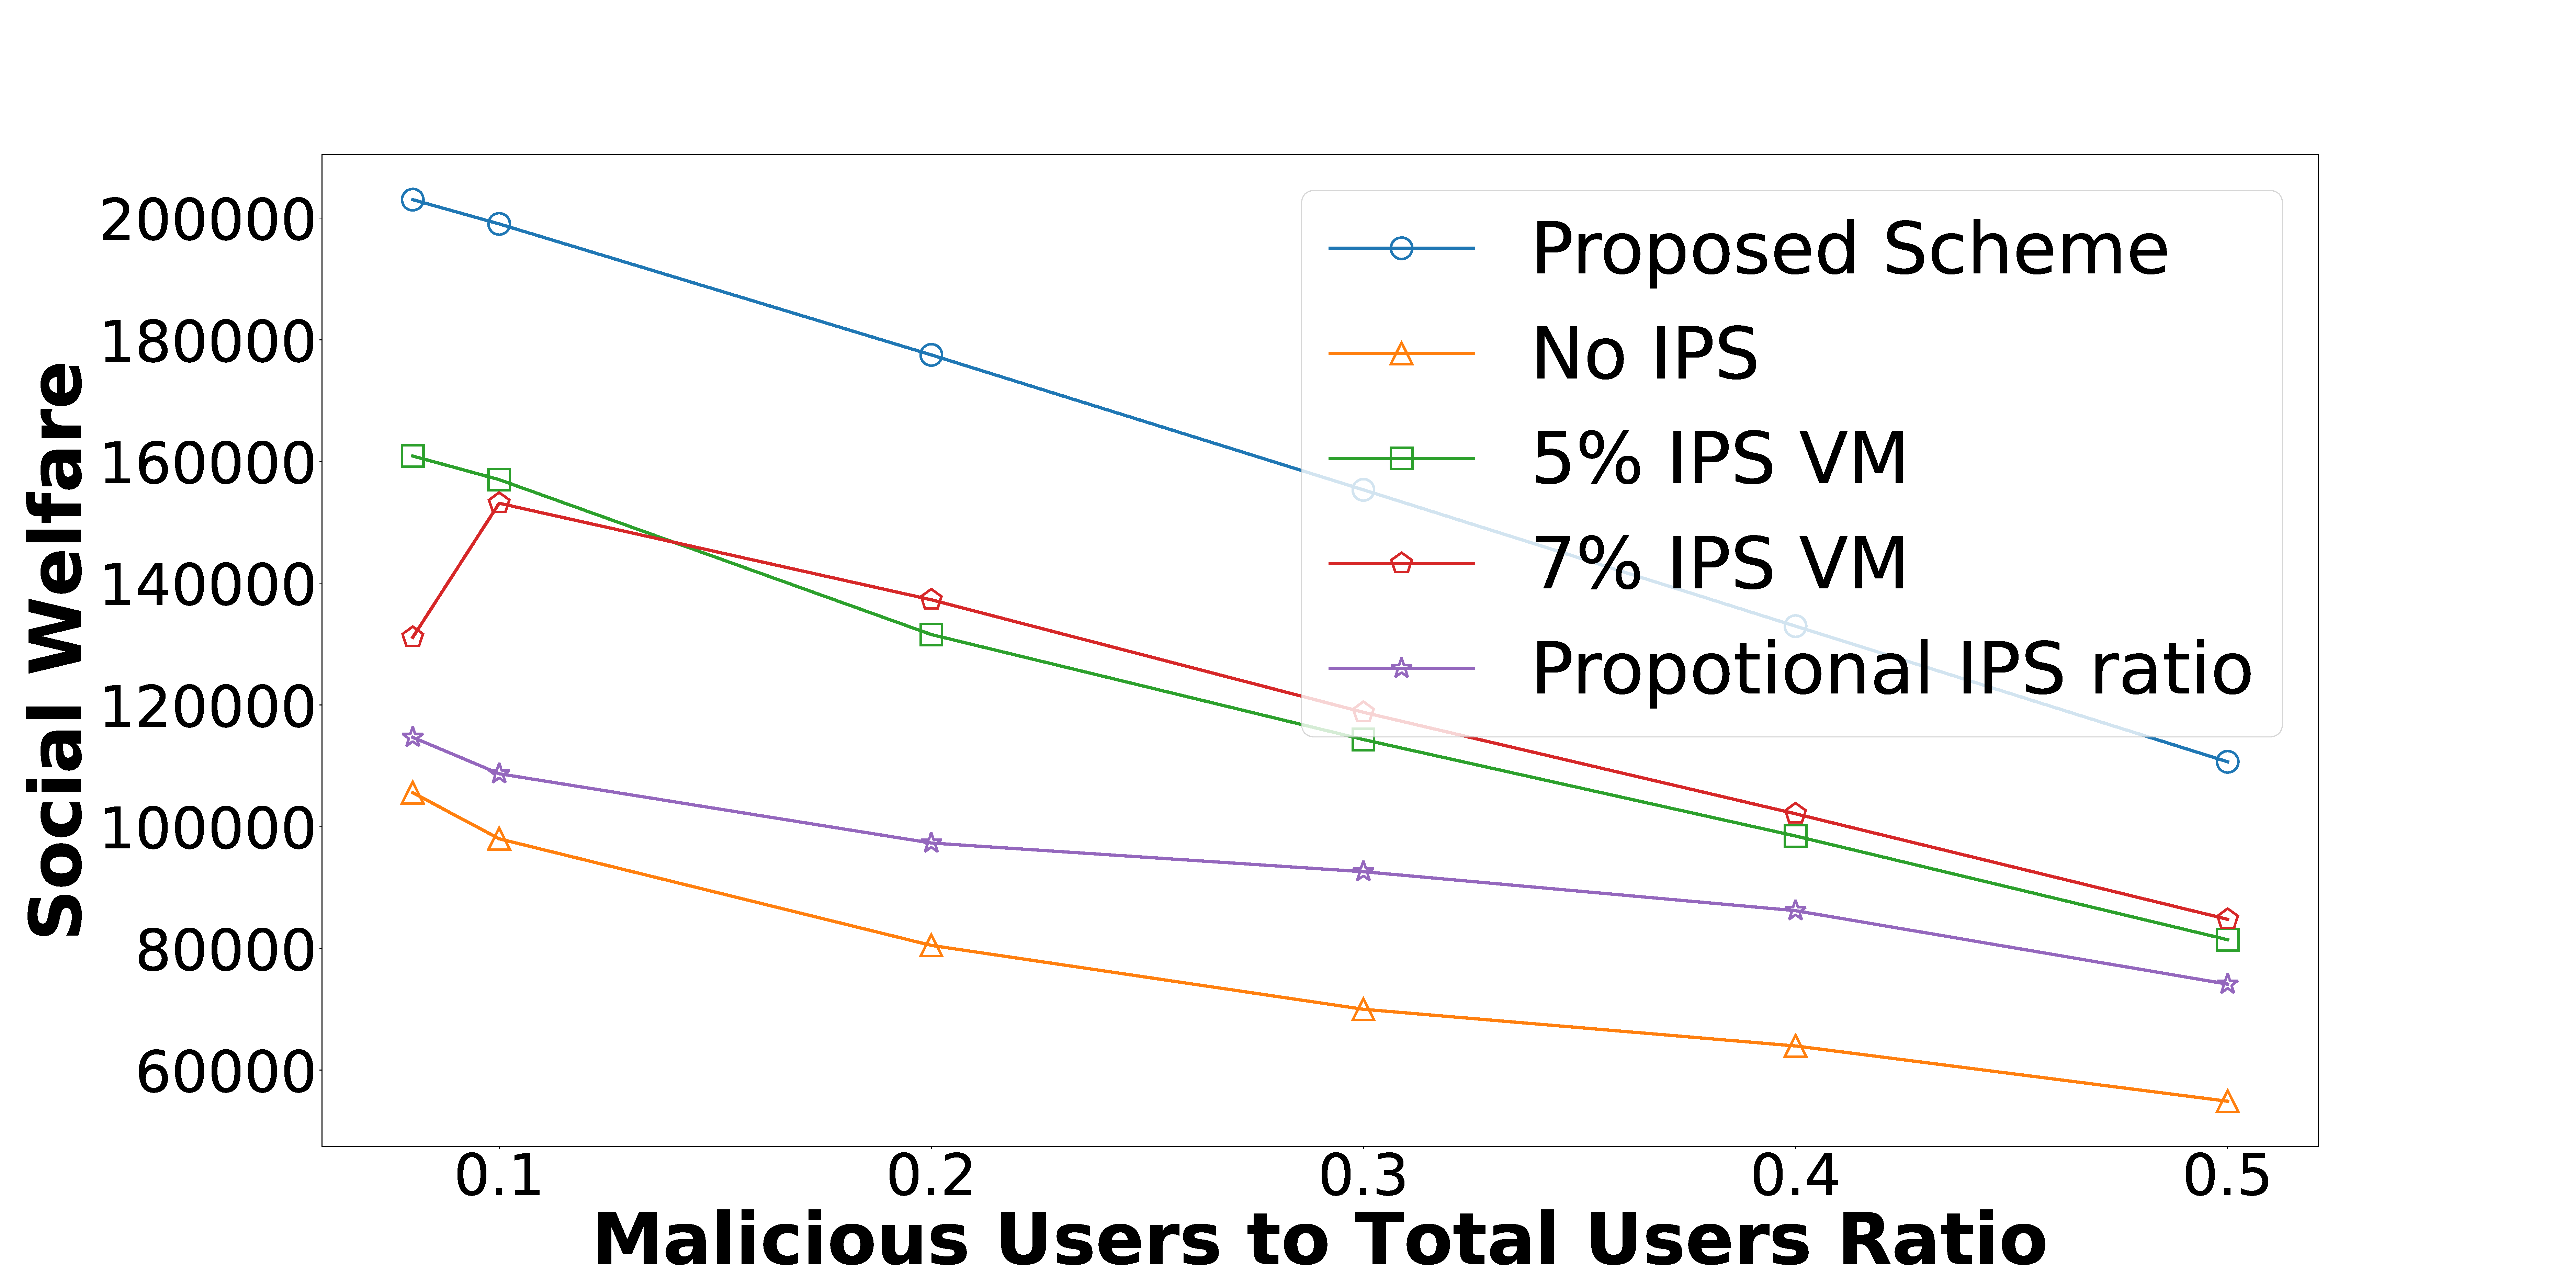
\includegraphics[width=0.33\textwidth]{5GDDoS_Game_social_ratio_high_cvx.pdf}}
  \hfill
  \subfloat[ASP Utility\label{fig:ratio_asp_high}]{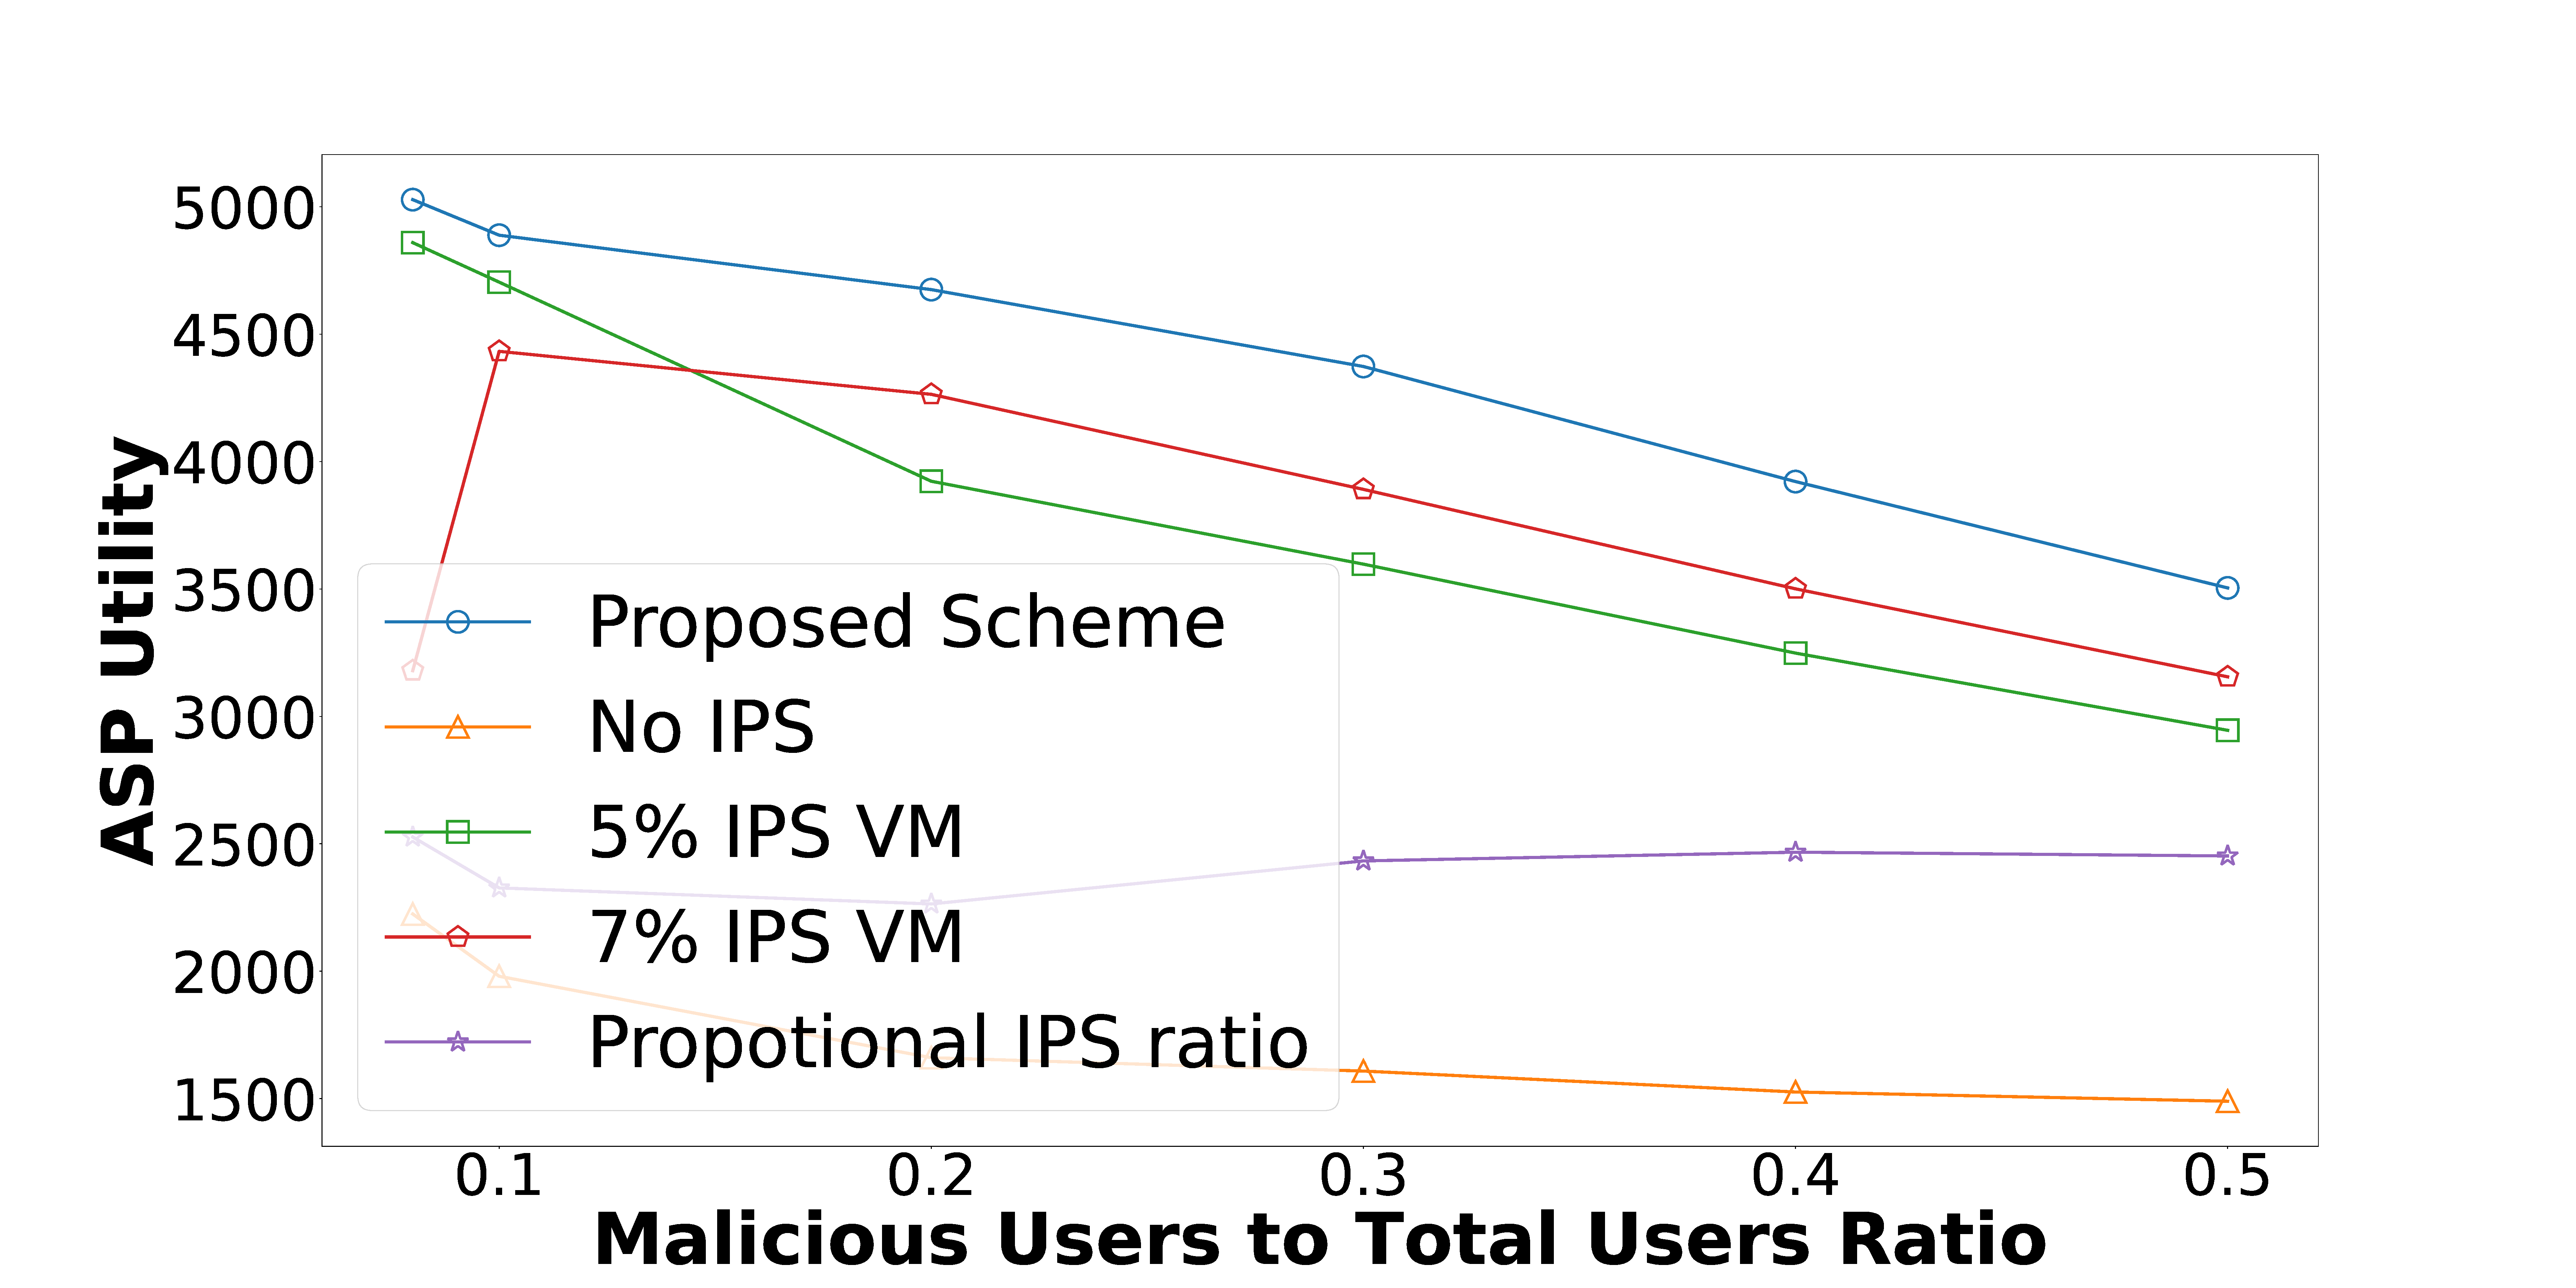
\includegraphics[width=0.33\textwidth] {5GDDoS_Game_asp_ratio_high_cvx.pdf}}
  \hfill
  \subfloat[MPO Utility\label{fig:ratio_mpo_high}]{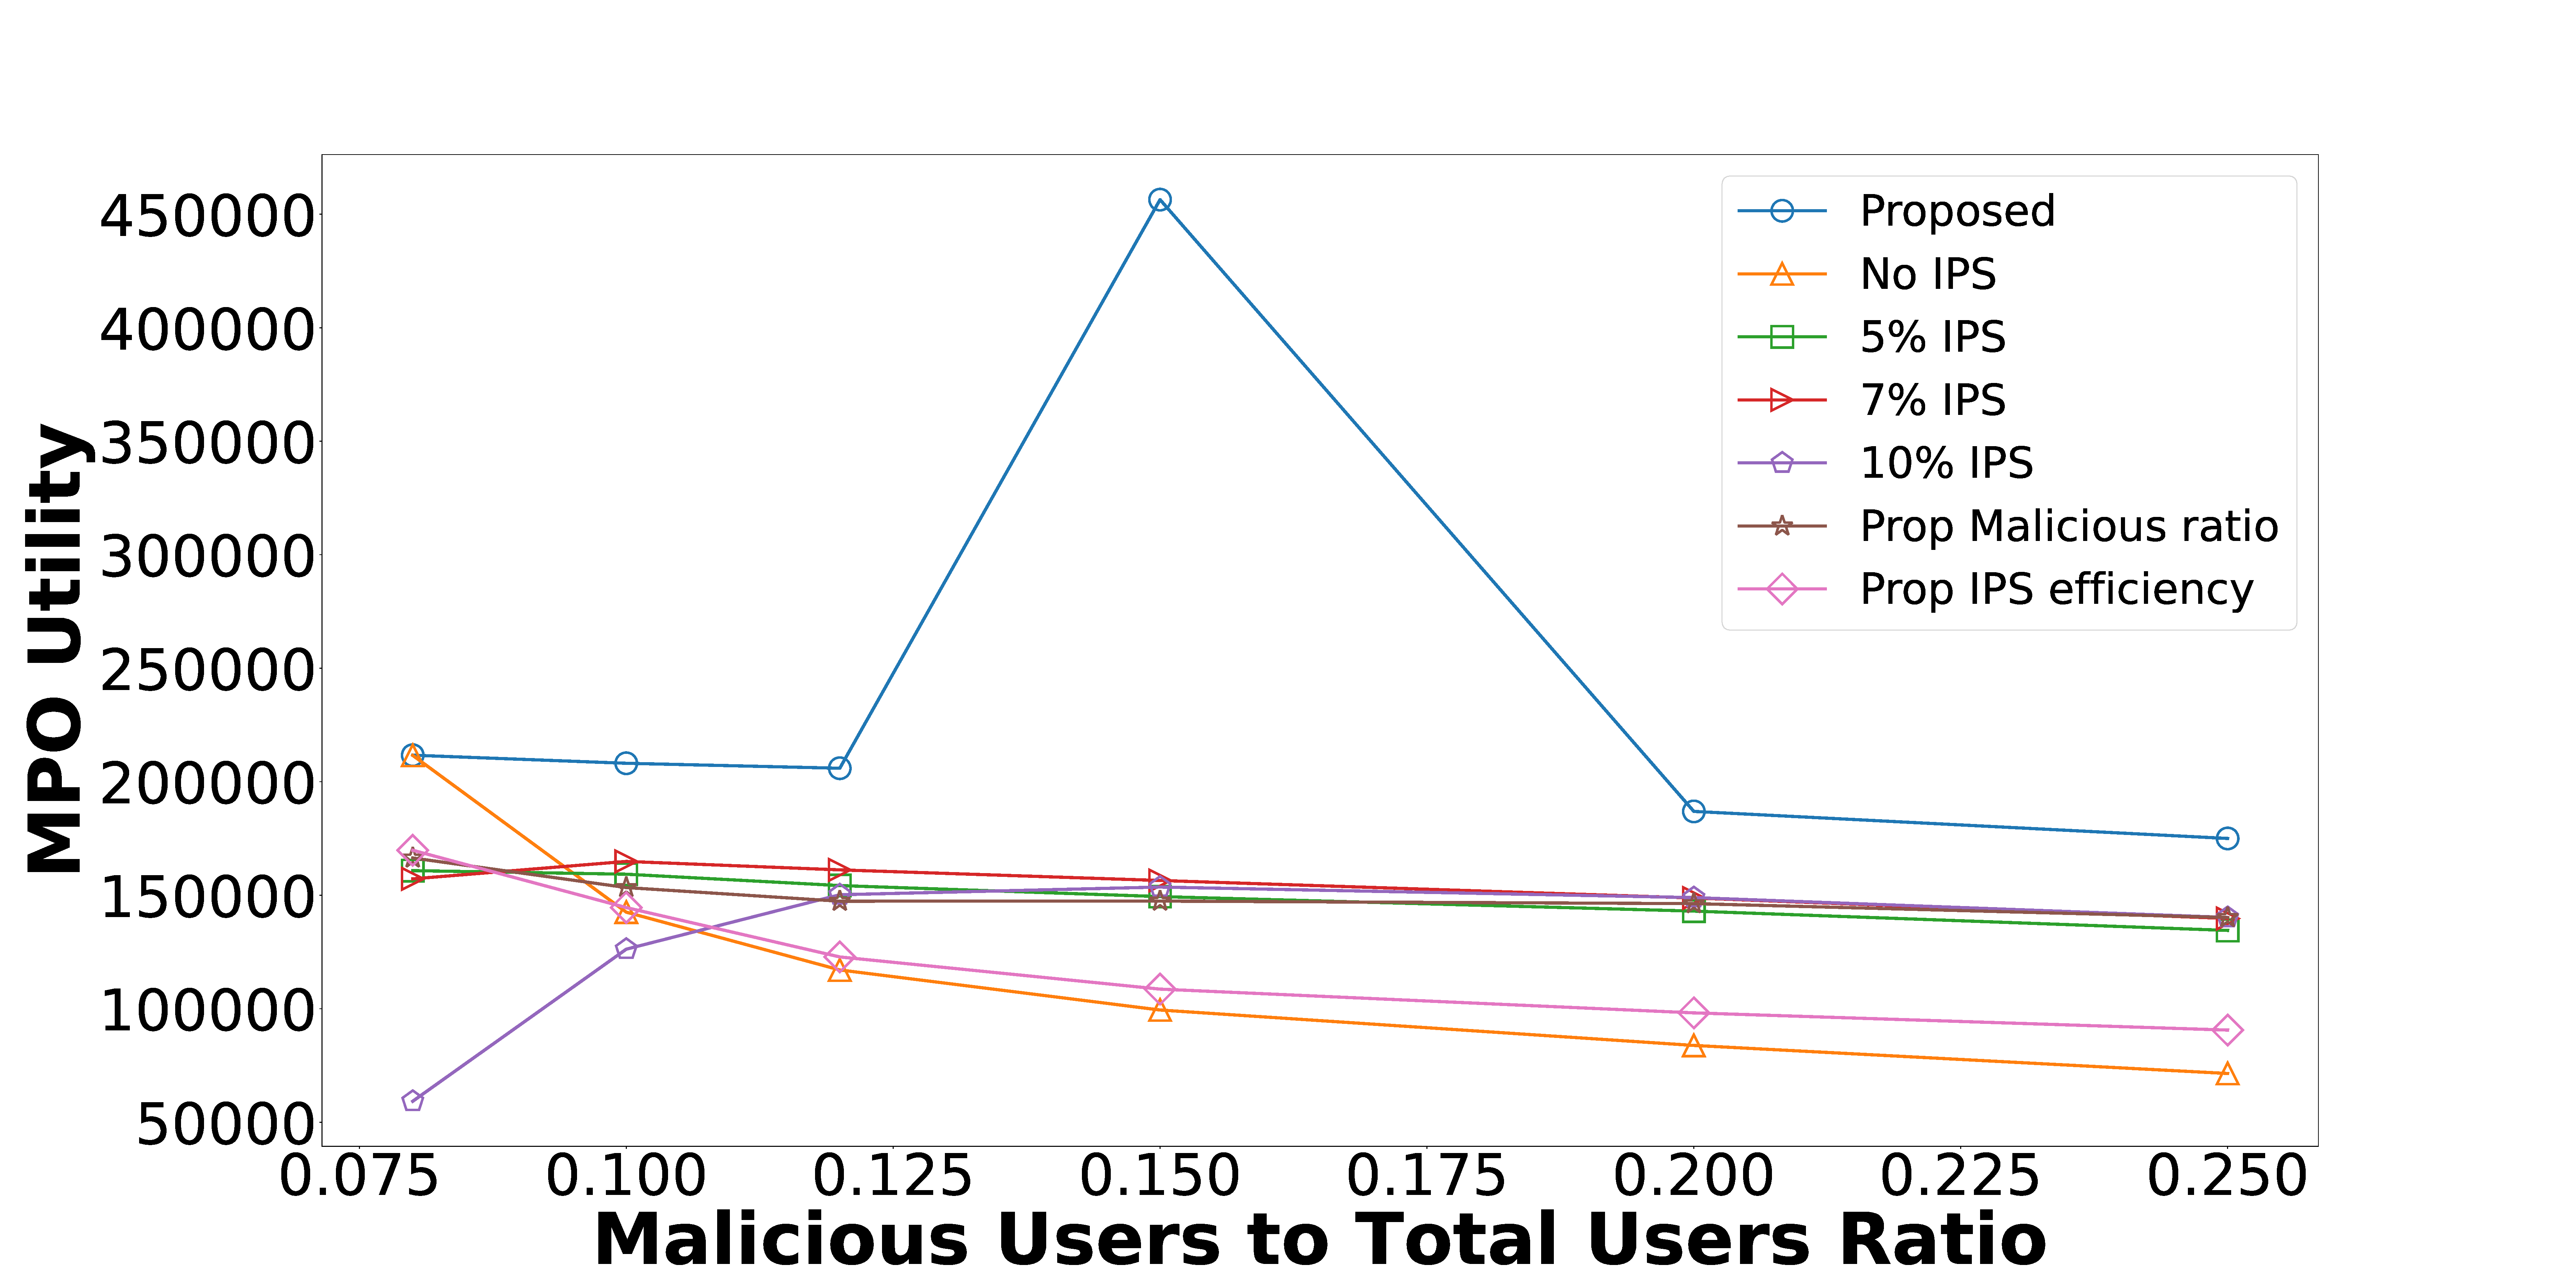
\includegraphics[width=0.33\textwidth]{5GDDoS_Game_MPO_ratio_high_cvx.pdf}}
\label{fig:ratio_high}
\caption{Different Malicious Users to Total Users Ratio of High Workload EUs}
\end{figure*}

\textbf{ASP with high workload EUs}:  In this case, when the workload of EUs are high, by \cref{eqn:service_rate}, the service rate would be low with default parameters (ratio = 0.1). Therefore, in this case, the interception rate would be higher than the service rate, and the ASPs tend to deploy more IPS VMs. However, when the number of malicious users is low, the IPS VMs can intercept fewer malicious requests, and the interception rate would be lower than the service rate. As the number of malicious users increases, the behavior of the ASPs changes at a specific point, which is the point where the interception rate and the service rate intersects. 

When the number of malicious users are low, the ASP will tend to deploy fewer IPS VM. In this case, if the ASP deploys excessive IPS VMs, it would crowd out VMs serving EUs. The scheme \textit{No IPS} has higher utility when the number of malicious users are low. As for \textit{10\% IPS VM}, the utility curve in \Cref{fig:ratio_asp_high} is far lower than \textit{5\% IPS VM} because it deploys redundant IPS VMs. Moreover, when the ratio of malicious to total users increases, the interception rate increases and exceed the service rate. Therefore, the ASP tends to deploy more IPS VMs. We observe that the curve of \textit{No IPS} scheme and the utility curve of \textit{5\% IPS VM} and \textit{7\% IPS VM} intersects. Also, when the malicious ratio increases, the \textit{10\% IPS VM} scheme has better utility than the \textit{5\% IPS VM} scheme. 

As for the scheme \textit{Proportional malicious ratio}, when the malicious ratio is low, \textit{Proportional malicious ratio} deploys fewer IPS VMs, so the utility is lower than \textit{5\% IPS VM}. However, when the number of malicious users increases, the \textit{Proportional malicious ratio} deploys more IPS VMs than \textit{5\% IPS VM} and \textit{10\% IPS VM}, and the ASPs' utility is higher than the scheme mentioned above. In addition, the \textit{Proposed Scheme} outperformed other schemes in \Cref{fig:ratio_soc_high}, \Cref{fig:ratio_asp_high}, and \Cref{fig:ratio_mpo_high} due to the optimal IPS deployment.

% ratio low
\begin{figure*}[!]
\captionsetup{justification=centering}
  \subfloat[Social Welfare\label{fig:ratio_soc_low}]{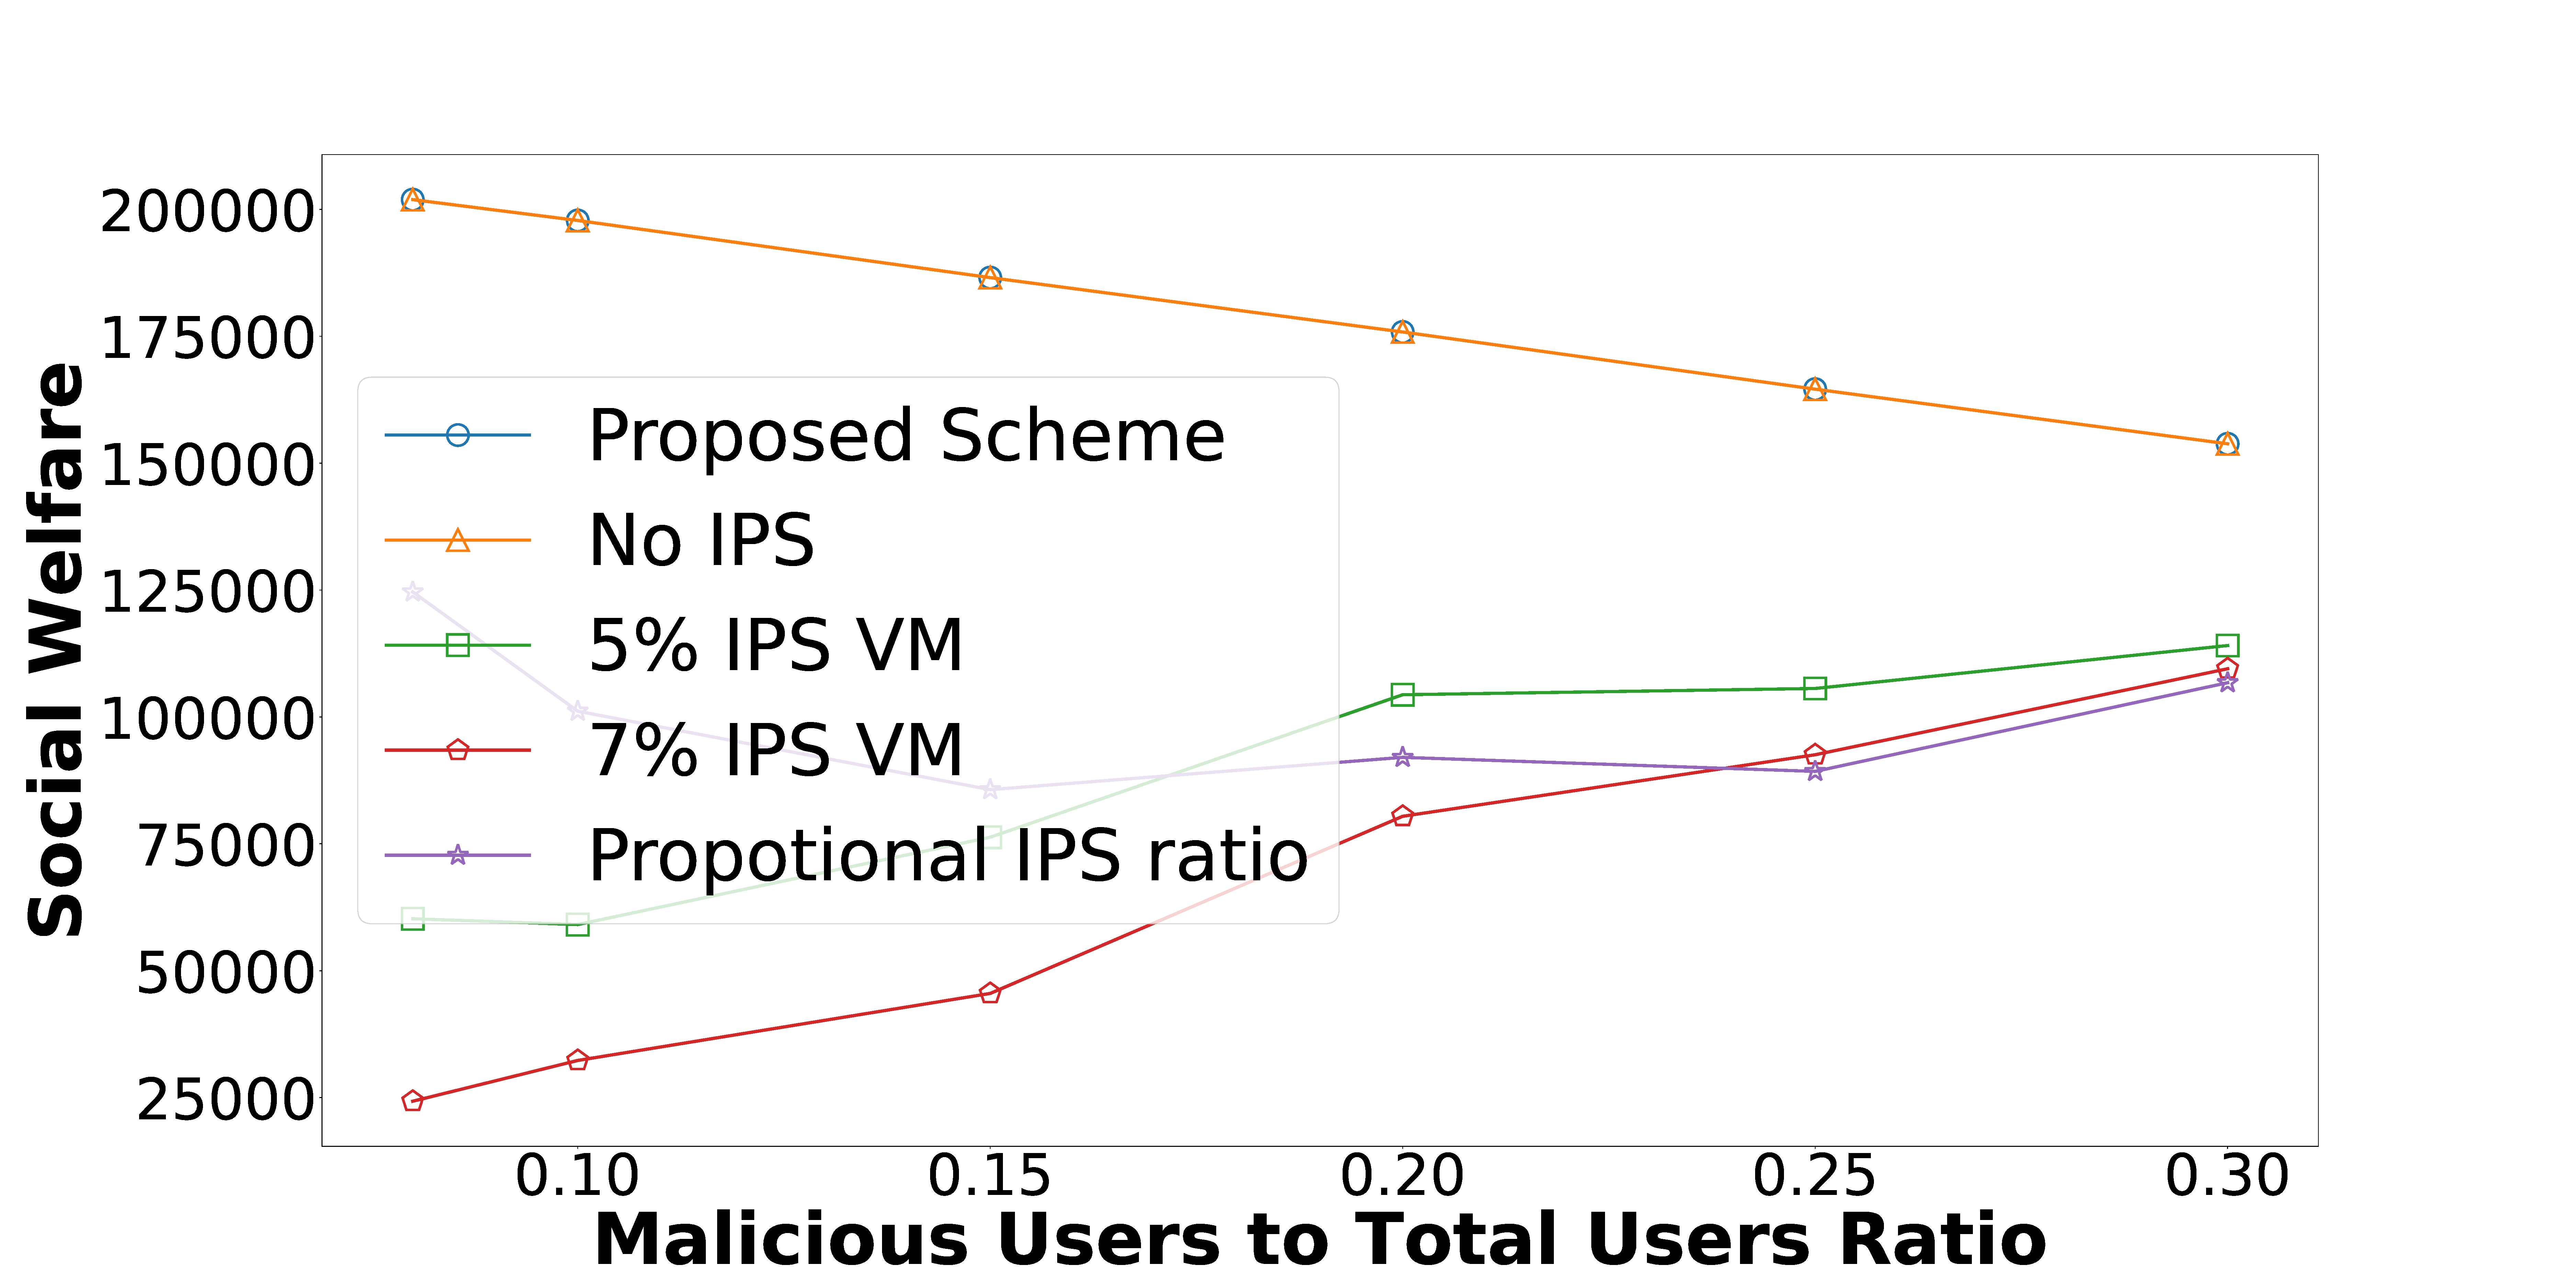
\includegraphics[width=0.33\textwidth]{5GDDoS_Game_social_ratio_low_cvx.pdf}}
  \hfill
  \subfloat[ASP Utility\label{fig:ratio_asp_low}]{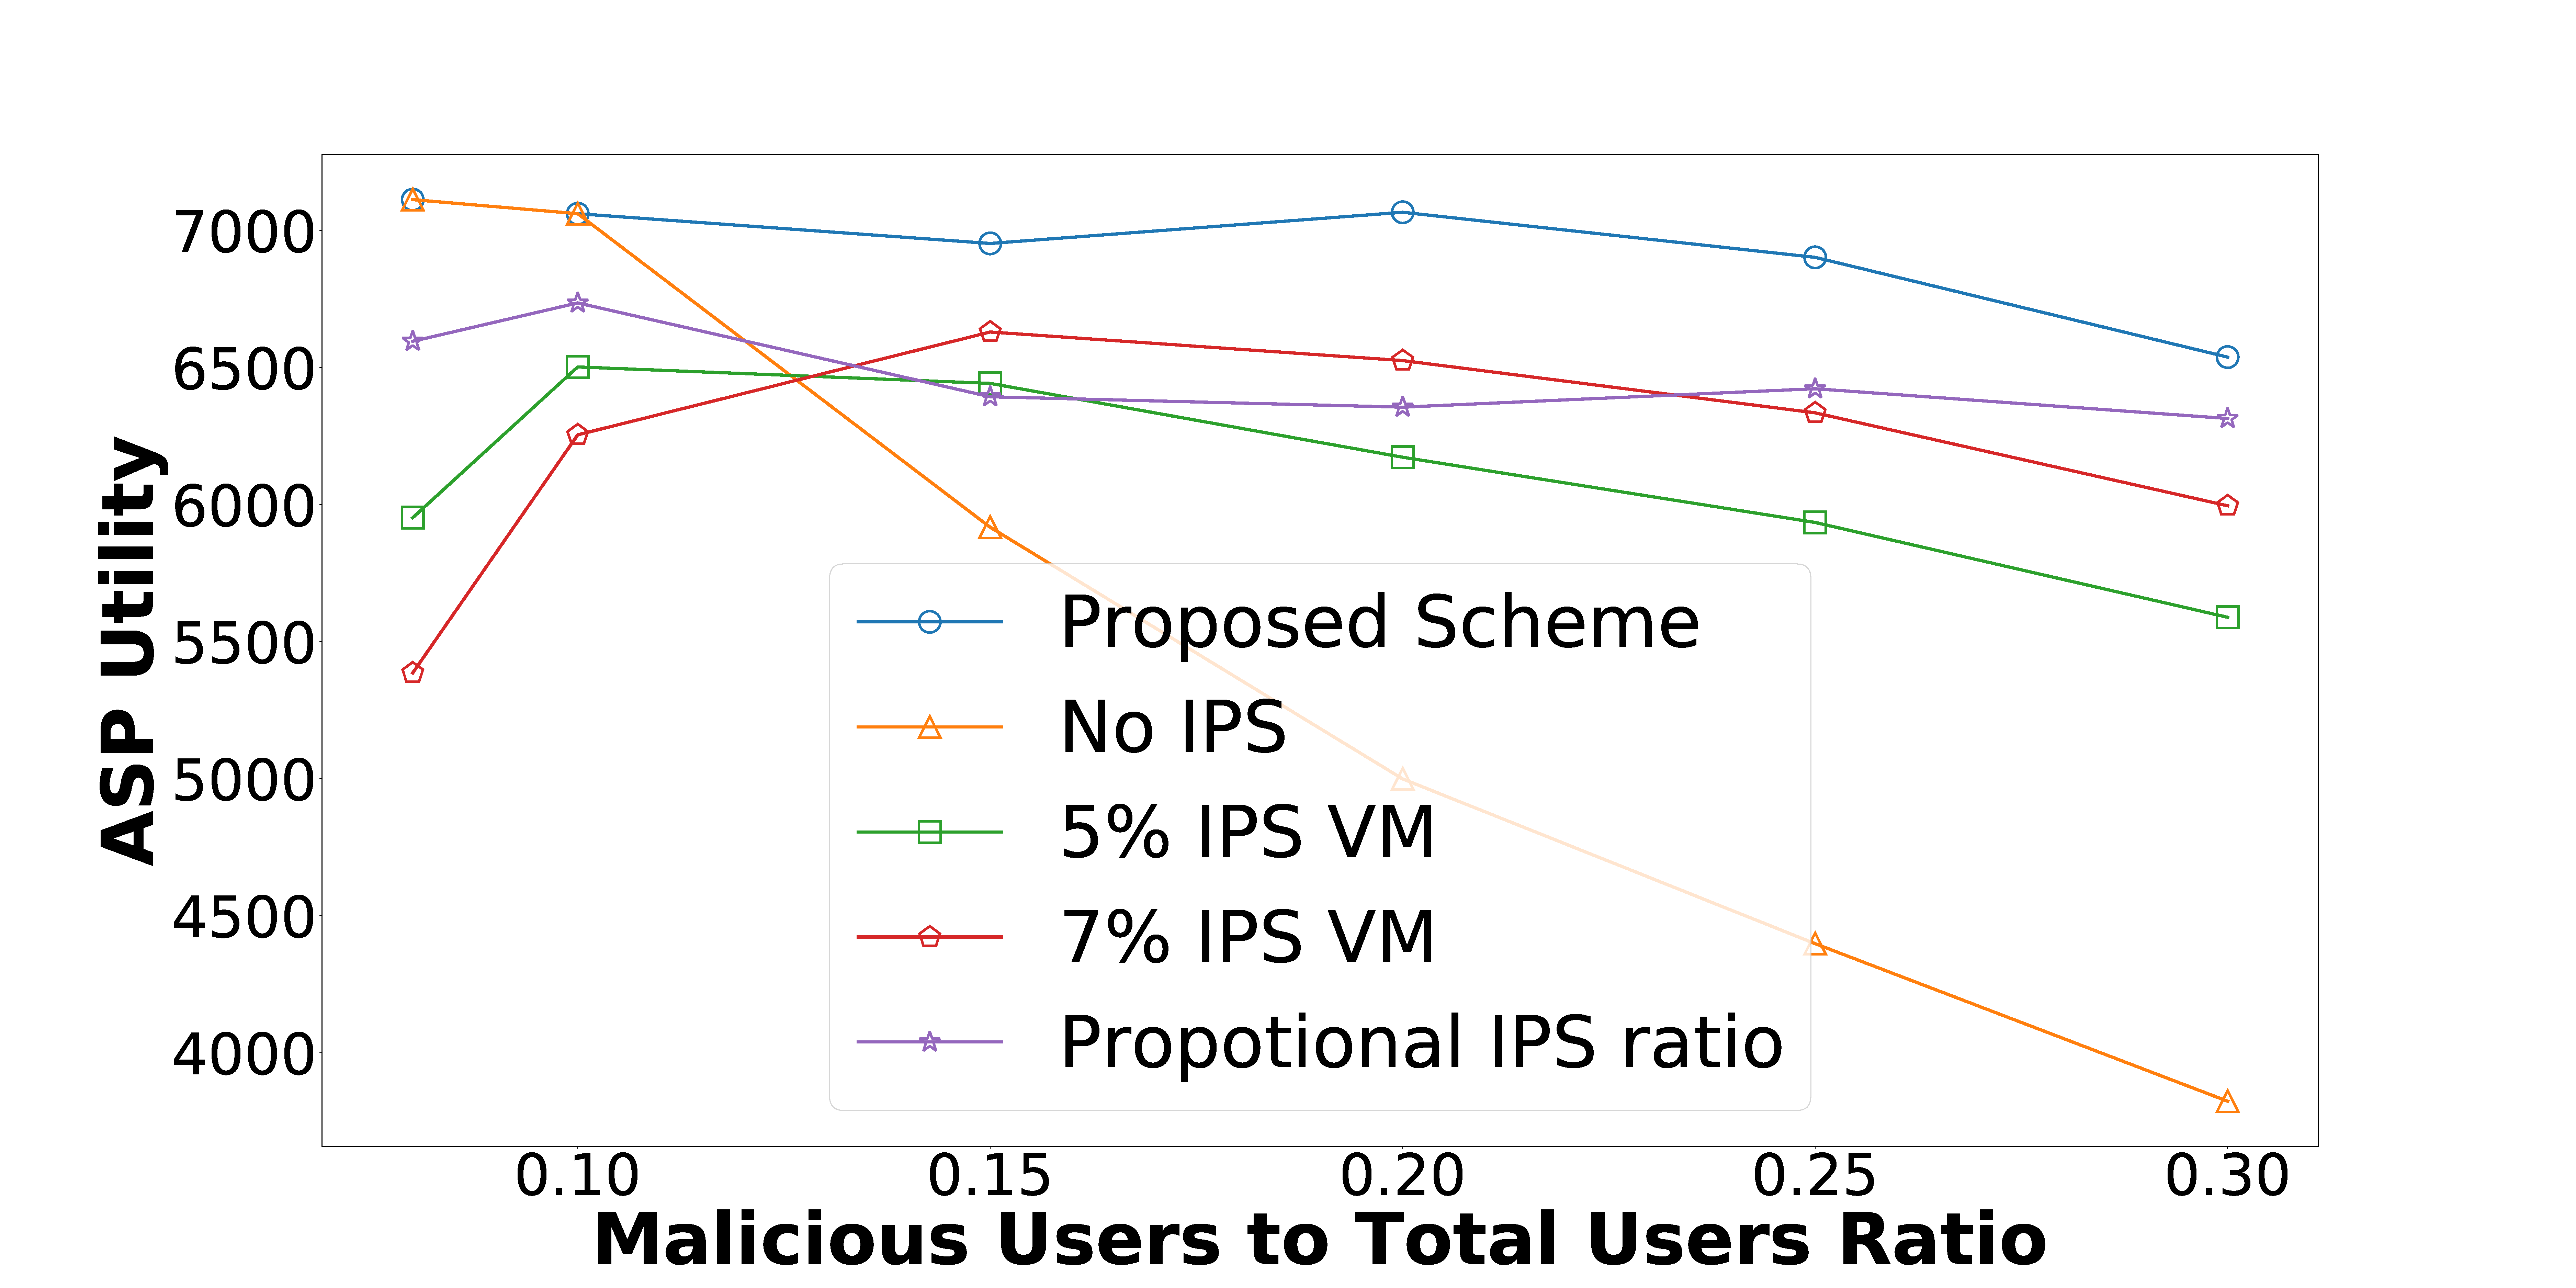
\includegraphics[width=0.33\textwidth] {5GDDoS_Game_asp_ratio_low_cvx.pdf}}
  \hfill
  \subfloat[MPO Utility\label{fig:ratio_mpo_low}]{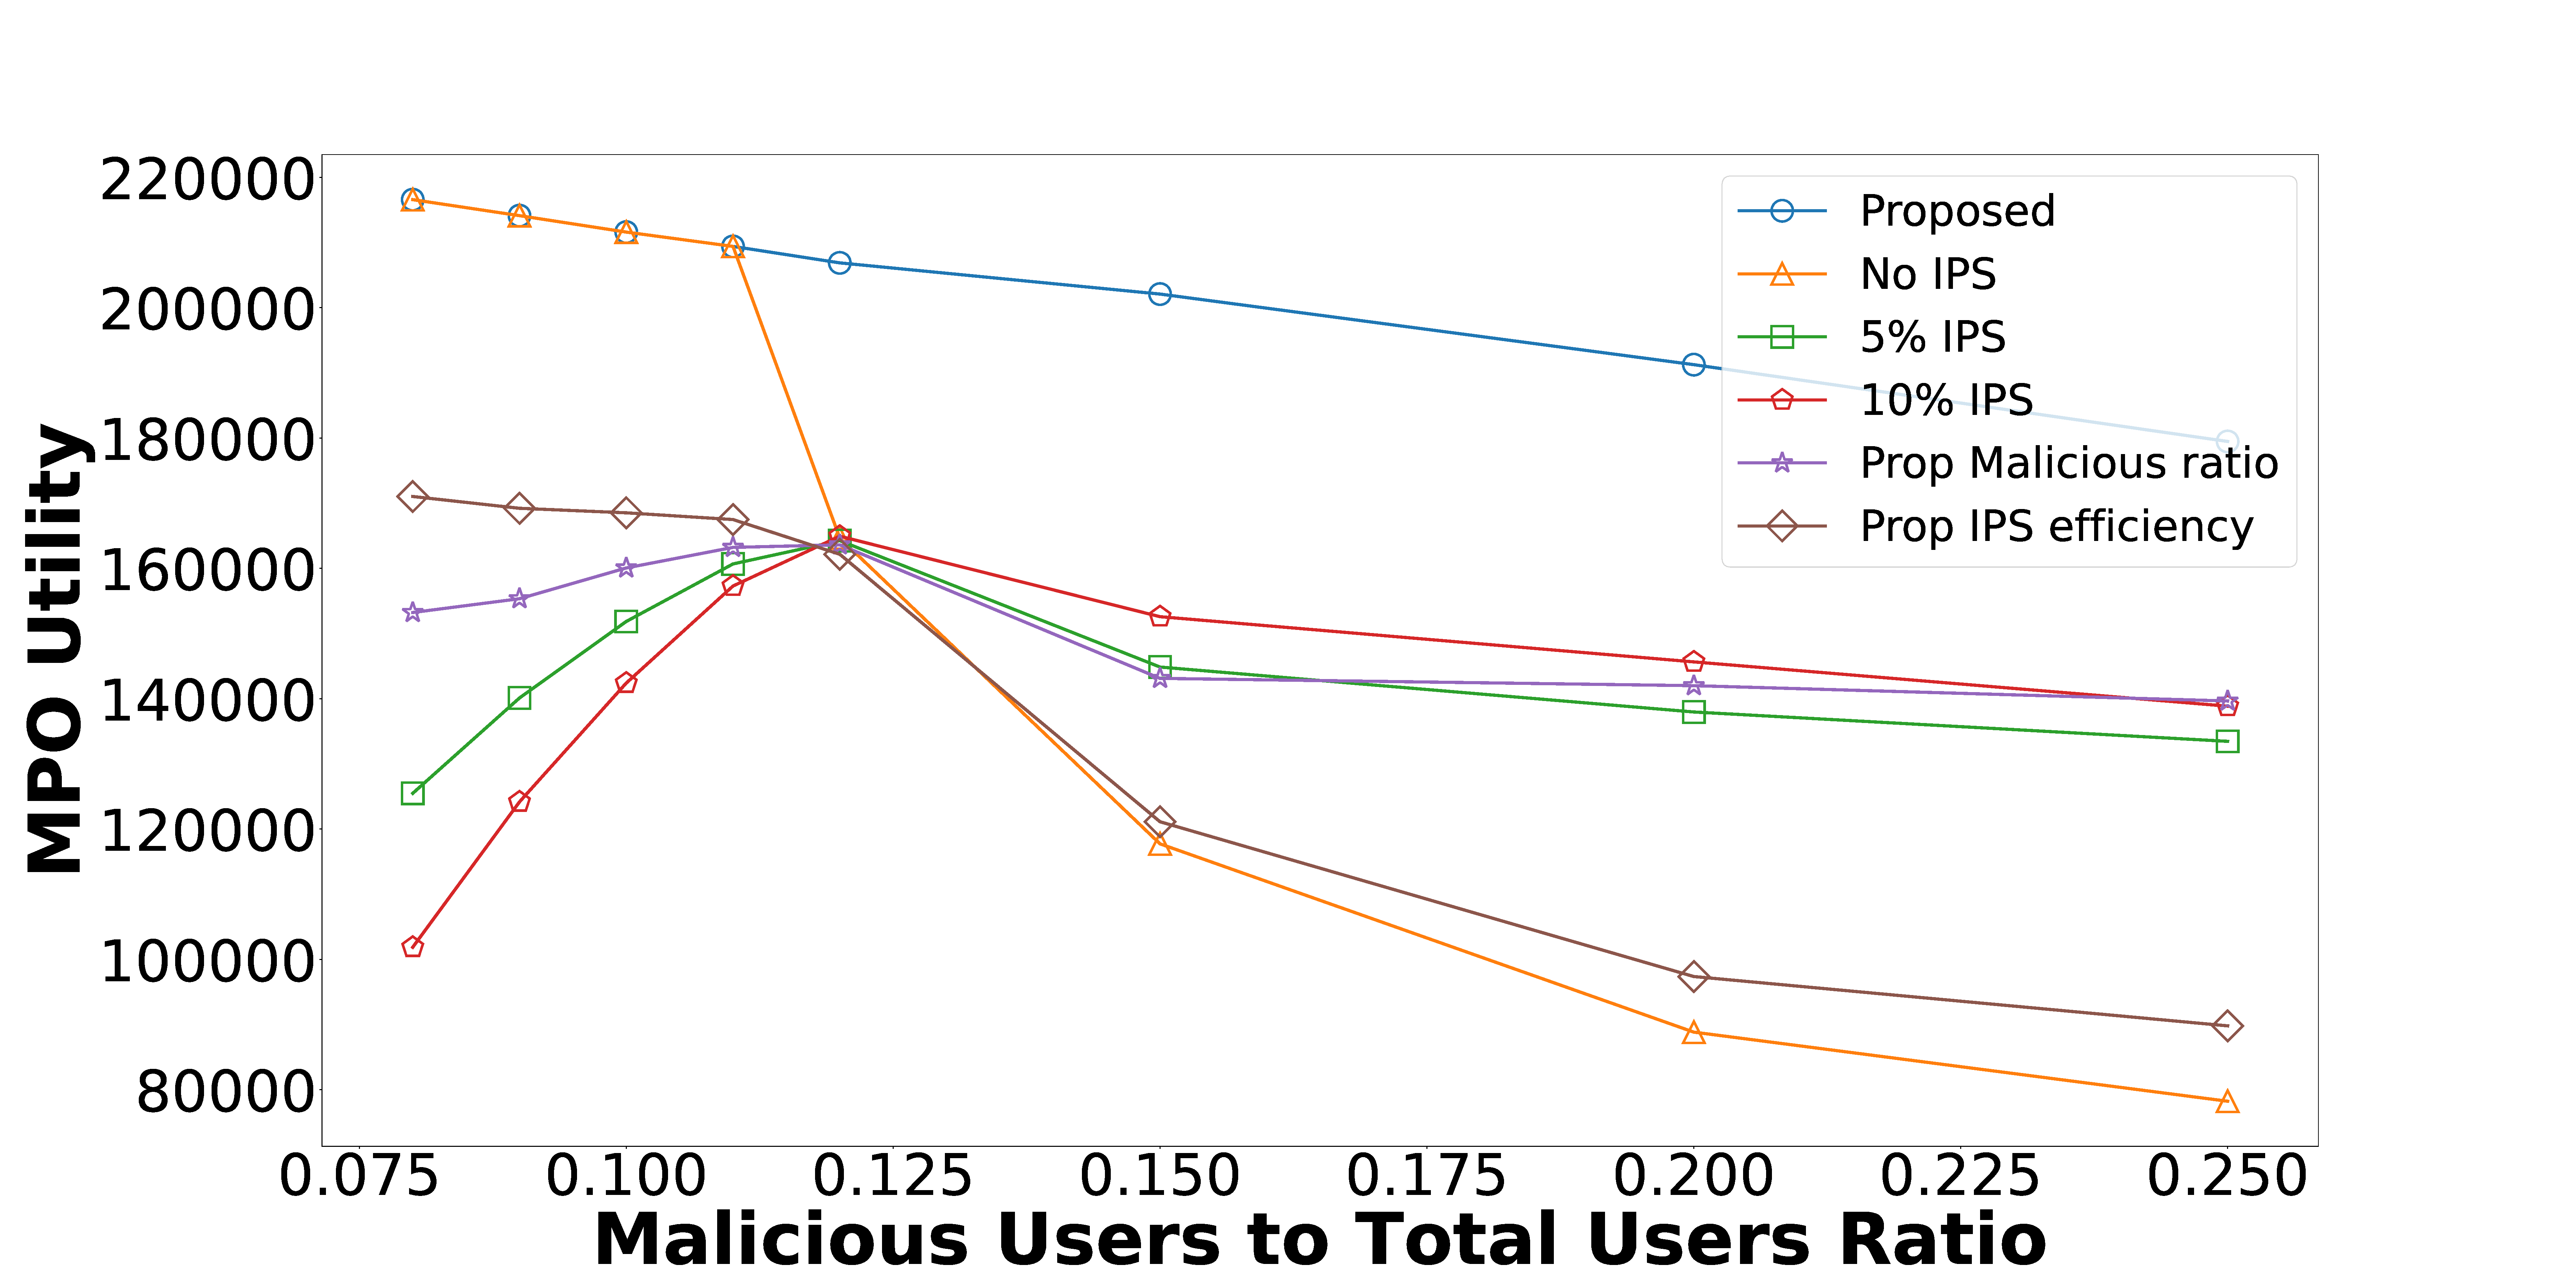
\includegraphics[width=0.33\textwidth]{5GDDoS_Game_MPO_ratio_low_cvx.pdf}}
\label{fig:ratio_low}
\caption{Different Malicious Users to Total Users Ratio of Low Workload EUs}
\end{figure*}


\textbf{ASP with low workload EUs}: In this case, when the workload of the EUs are low, by \cref{eqn:service_rate}, the service rate would be high in default parameters (ratio = 0.1). Also, the interception rate is lower than the service rate, so the ASPs tend to deploy fewer IPS VMs. However, when the number of malicious users increases, the deployed IPS VMs can intercept more malicious requests. As the number of malicious users increases, the behavior of the ASP changes at a specific point, which is the point where the interception rate and the service rate intersects. Despite this intersection point, the rest results are similar to the high-workload case.
% \textcolor{blue}{We omit the figure due to page limitations.}

% \textcolor{red}{Similar to the previous simulation, when the malicious users are low, the ASP tend to deploy fewer IPS VMs. The behaviors of \textit{No IPS} and \textit{Proposed Scheme} are identical in this case when malicious users are low. Moreover, the \textit{5\% IPS VM} has higher utility than \textit{7\% IPS VM} and \textit{10\% IPS VM} when malicious users are low because ASPs have less incentive to deploy IPS VMs. In addition, the \textit{Proportional malicious ratio} has deployed lower IPS VMs when the malicious ratio is low, so the utility is higher than \textit{5\% IPS VM},  \textit{7\% IPS VM}, and \textit{10\% IPS VM}.}

% \textcolor{red}{
% When the number of malicious users rises, similar to the previous case, the ASPs tend to deploy more IPS VMs when the malicious ratio is high. In this case, \textit{10\% IPS VM} has the highest utility among other fixed ratio schemes. As for the \textit{Proportional malicious ratio} scheme, the scheme has lower utility when the number of malicious users is low. When the number of malicious users increases, the utility exceeds \textit{5\% IPS VM} and \textit{7\% IPS VM} because it deploys more IPS VMs. For example, when the ratio is $0.25$, the ASPs deploy $0.25 \times 30 \% = 7.5\%$ IPS VMs, which is higher than \textit{7\% IPS VM}. As a result, the utility is higher. Similarly, the \textit{Proposed Scheme} has outperformed other schemes in \Cref{fig:ratio_soc_low}, \Cref{fig:ratio_asp_low}, and \Cref{fig:ratio_mpo_low}.}

\subsection{Comparison between various IPS efficiency}
In this simulation, we compare different IPS VM deployment schemes on ASPs given various IPS efficiency $\nu$. Similar to the previous simulation, we discuss two different cases: ASP with high workload EUs and ASP with low workload EUs. The parameters of high and low workload EUs are mentioned in the previous simulation. We discuss the different characteristics of these two types of ASPs.

% eff high
\begin{figure*}[!]
\captionsetup{justification=centering}
  \subfloat[Social Welfare\label{fig:eff_soc_high}]{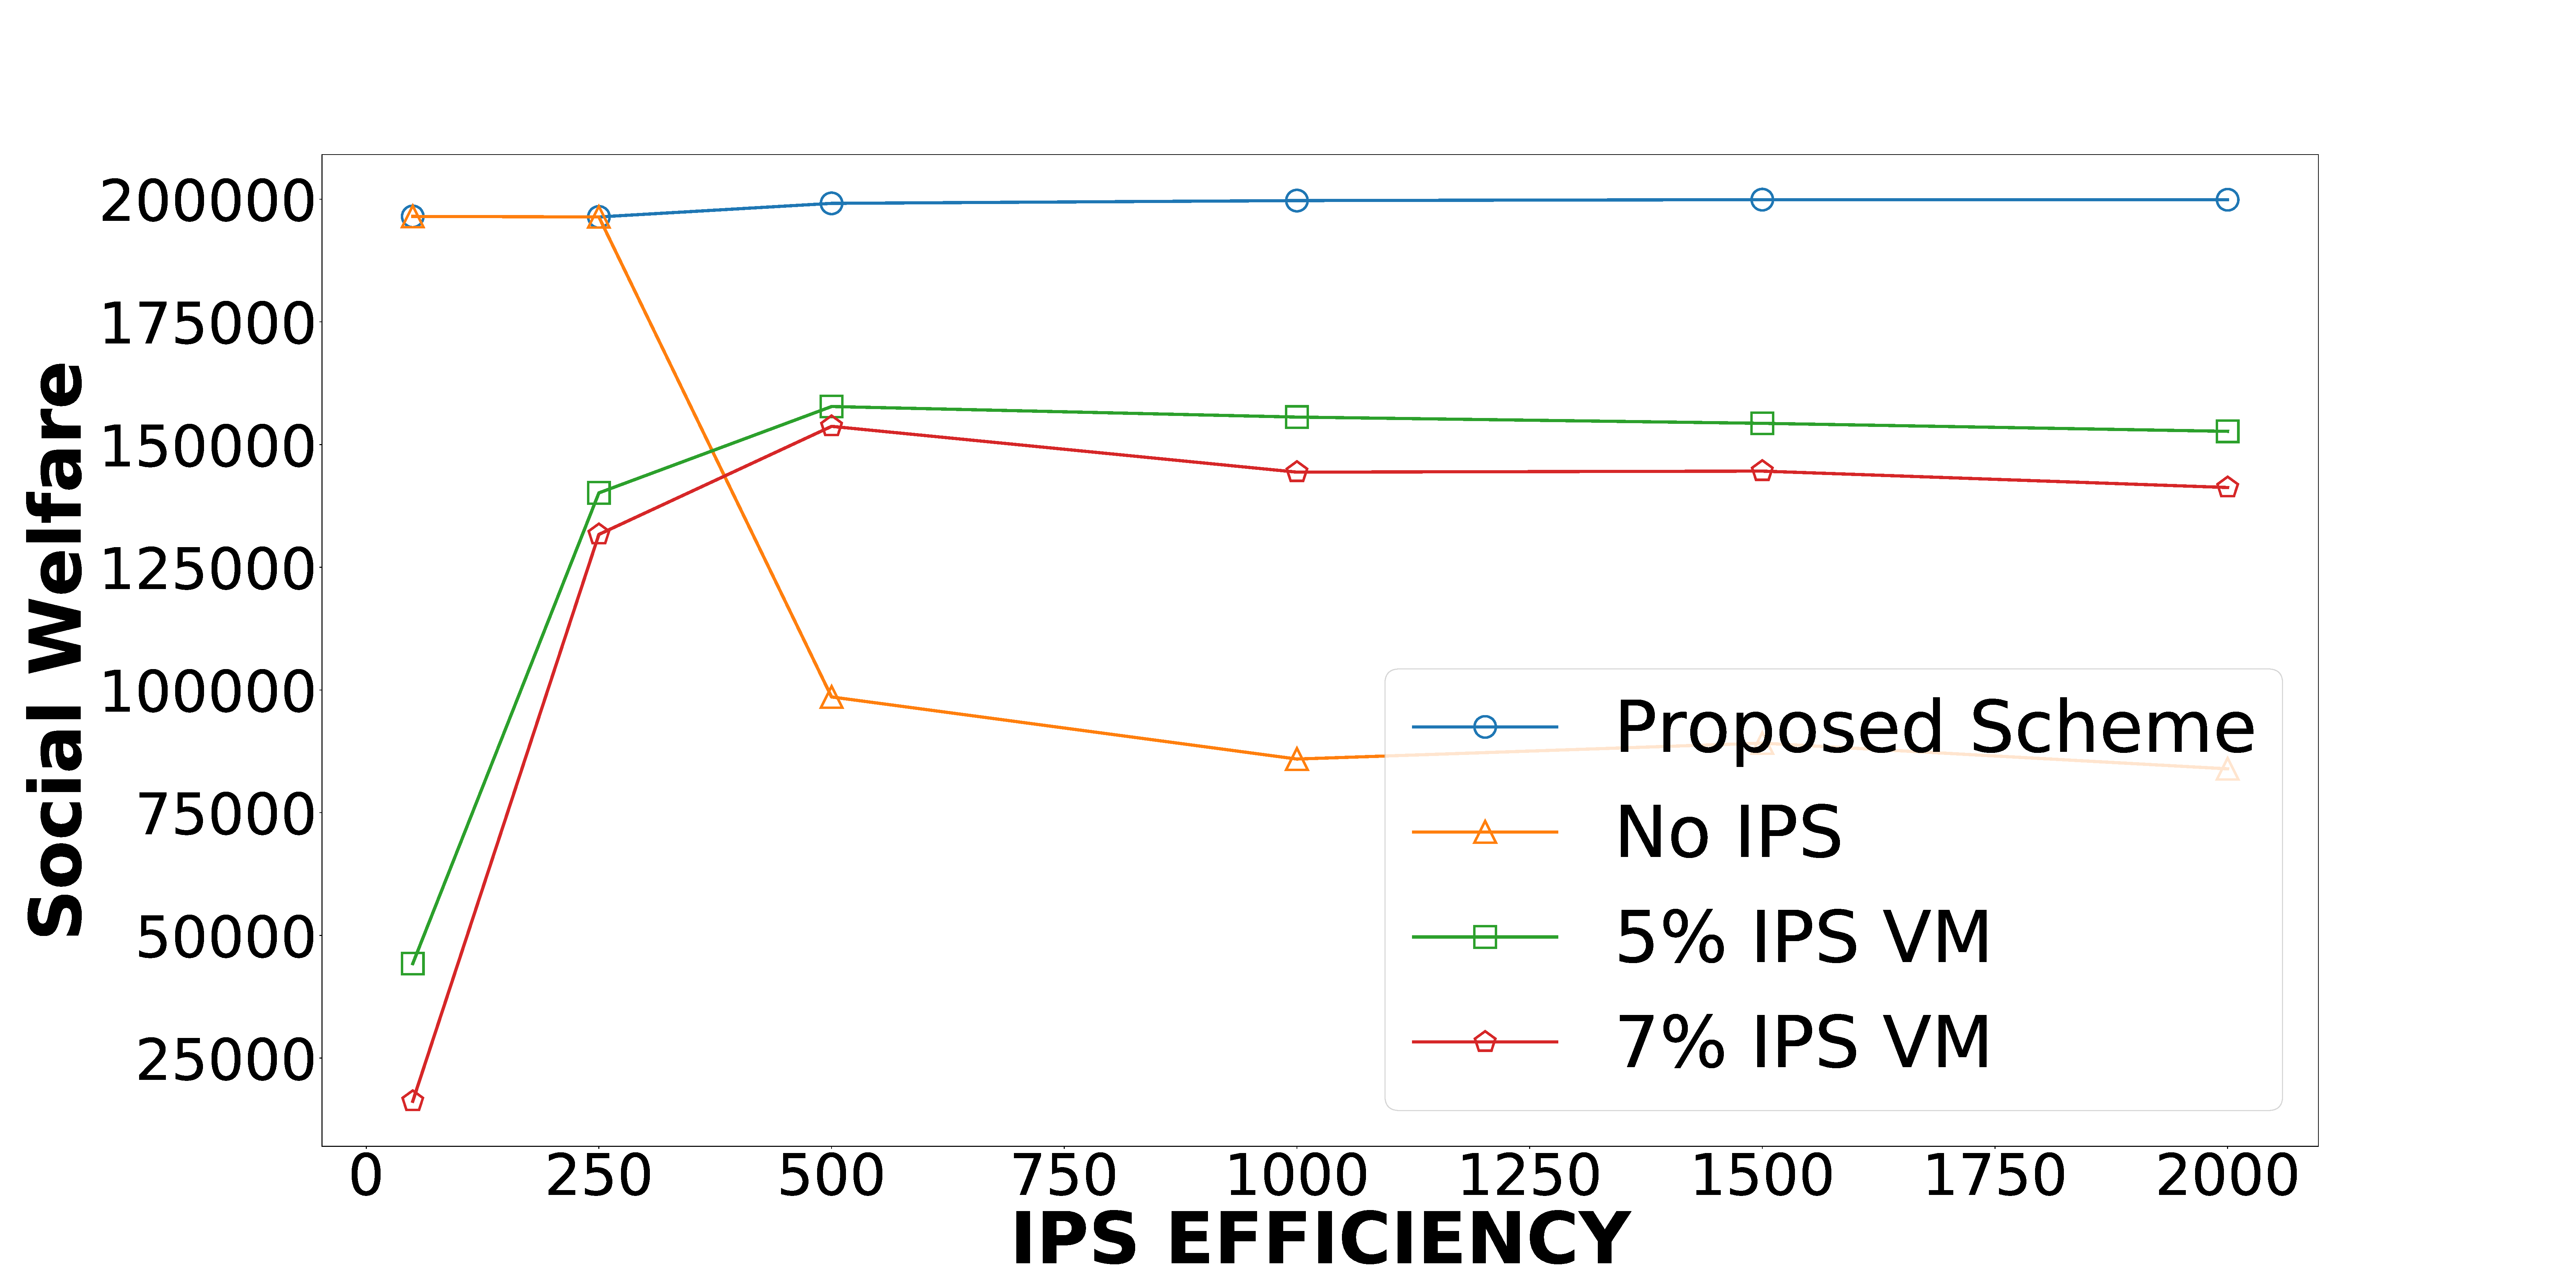
\includegraphics[width=0.33\textwidth]{5GDDoS_Game_social_efficiency_high_cvx.pdf}}
  \hfill
  \subfloat[ASP Utility\label{fig:eff_asp_high}]{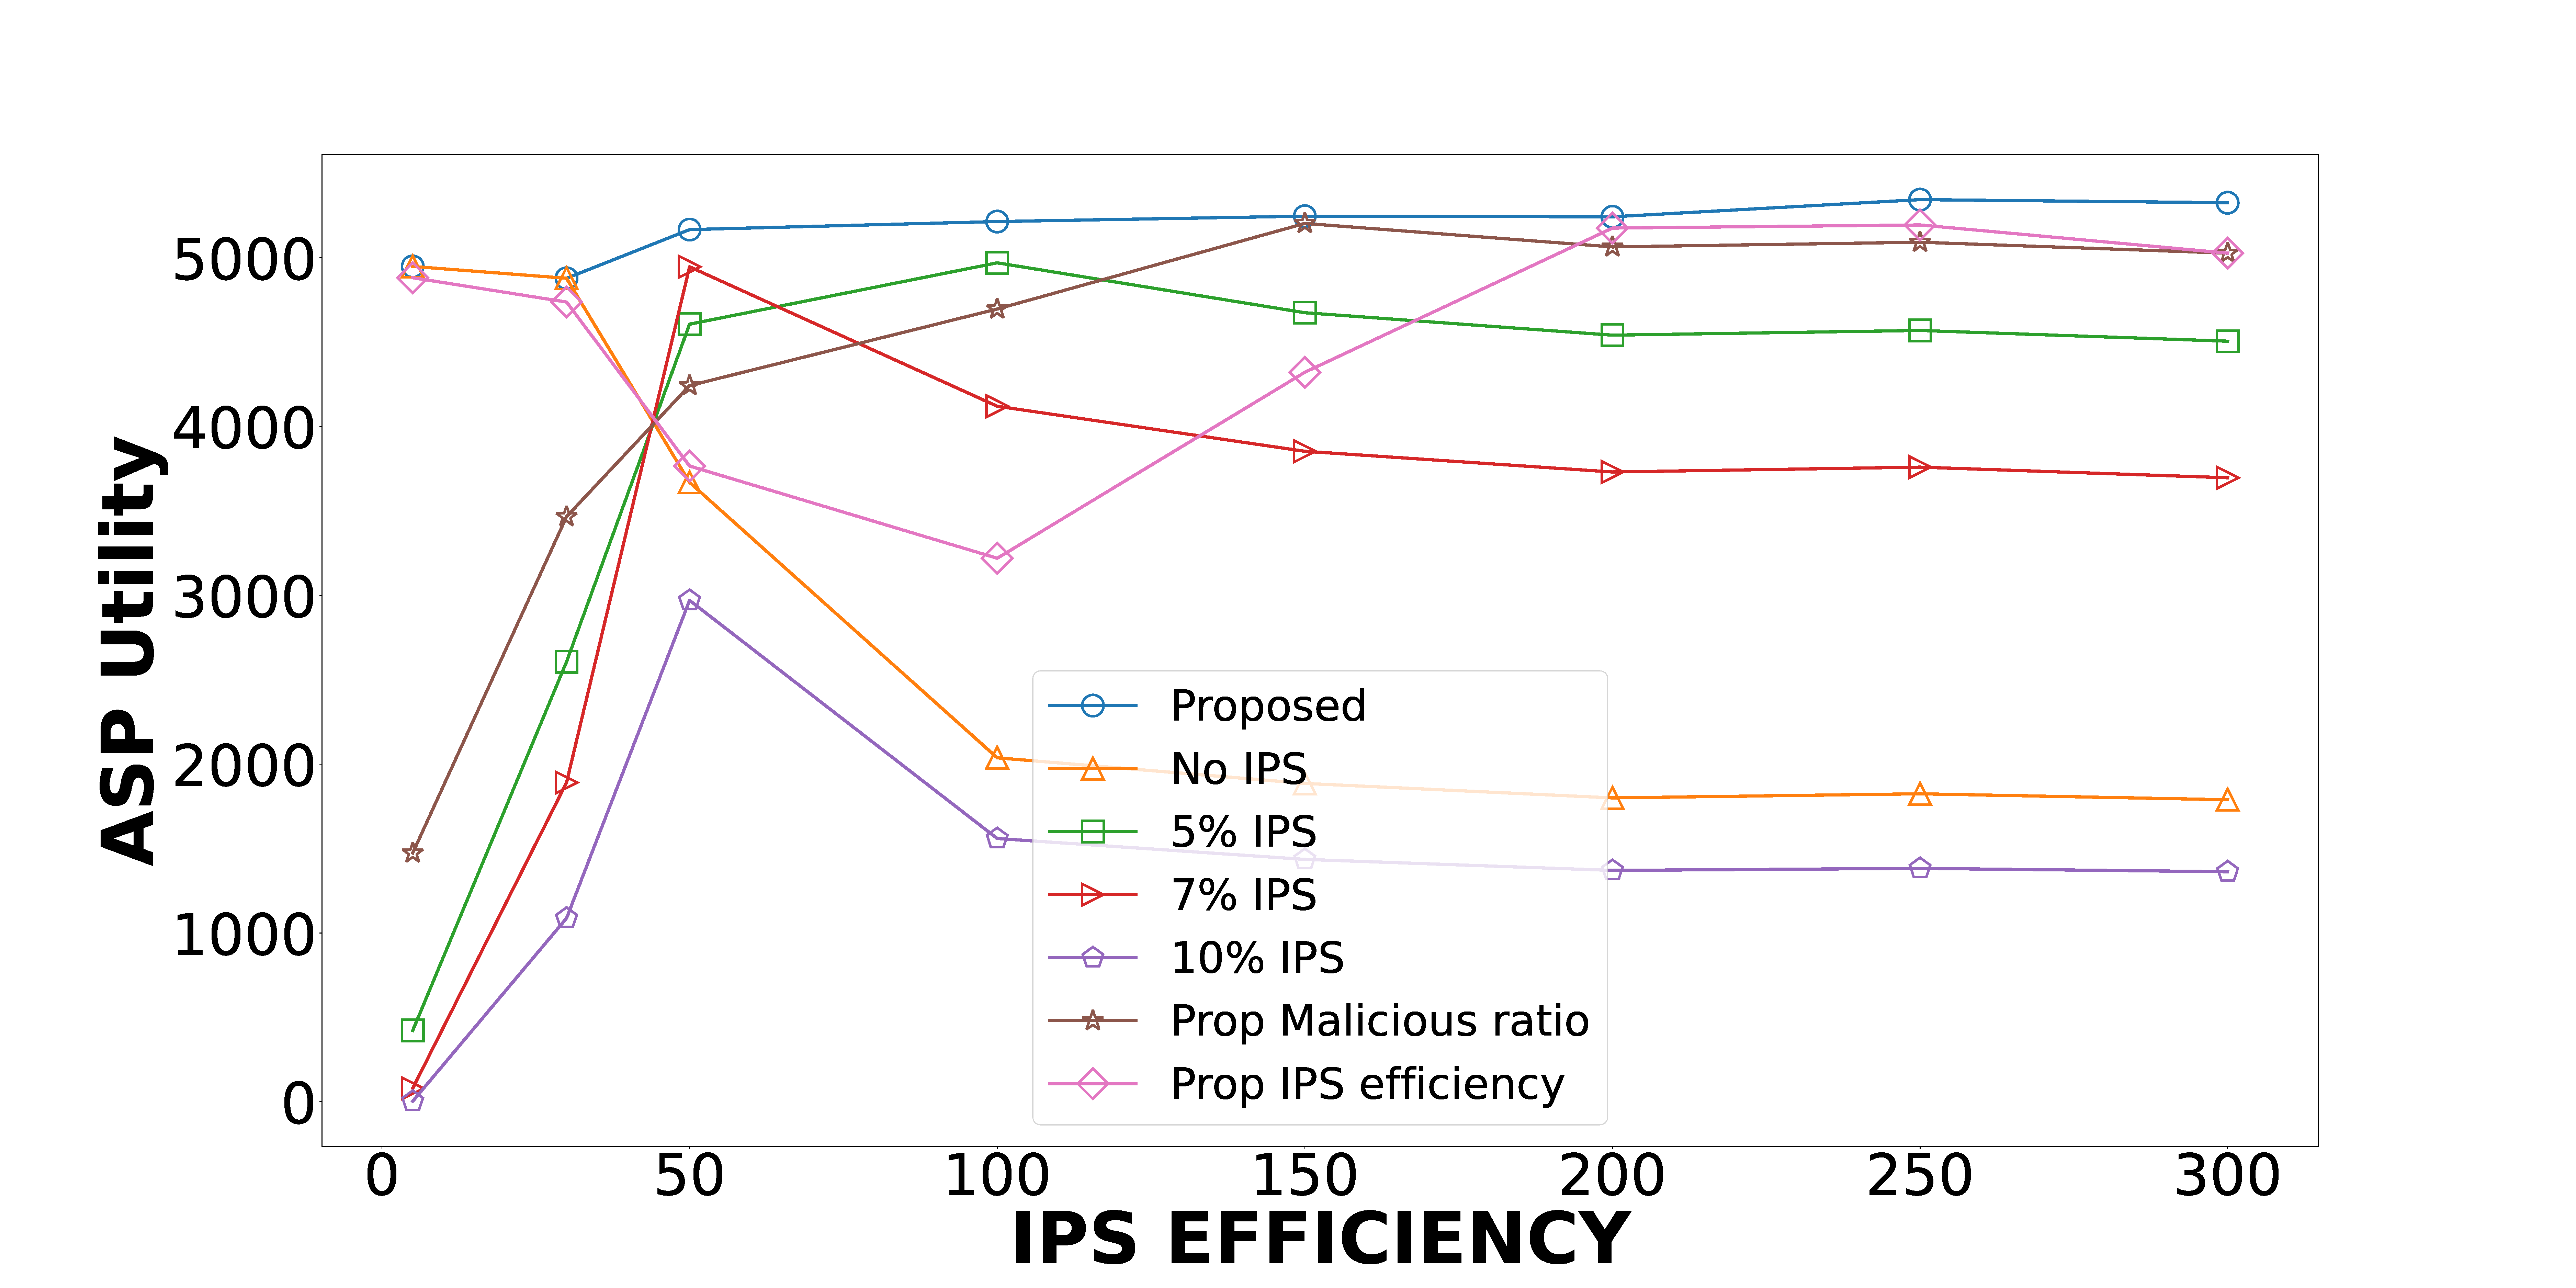
\includegraphics[width=0.33\textwidth] {5GDDoS_Game_asp_efficiency_high_cvx.pdf}}
  \hfill
  \subfloat[MPO Utility\label{fig:eff_mpo_high}]{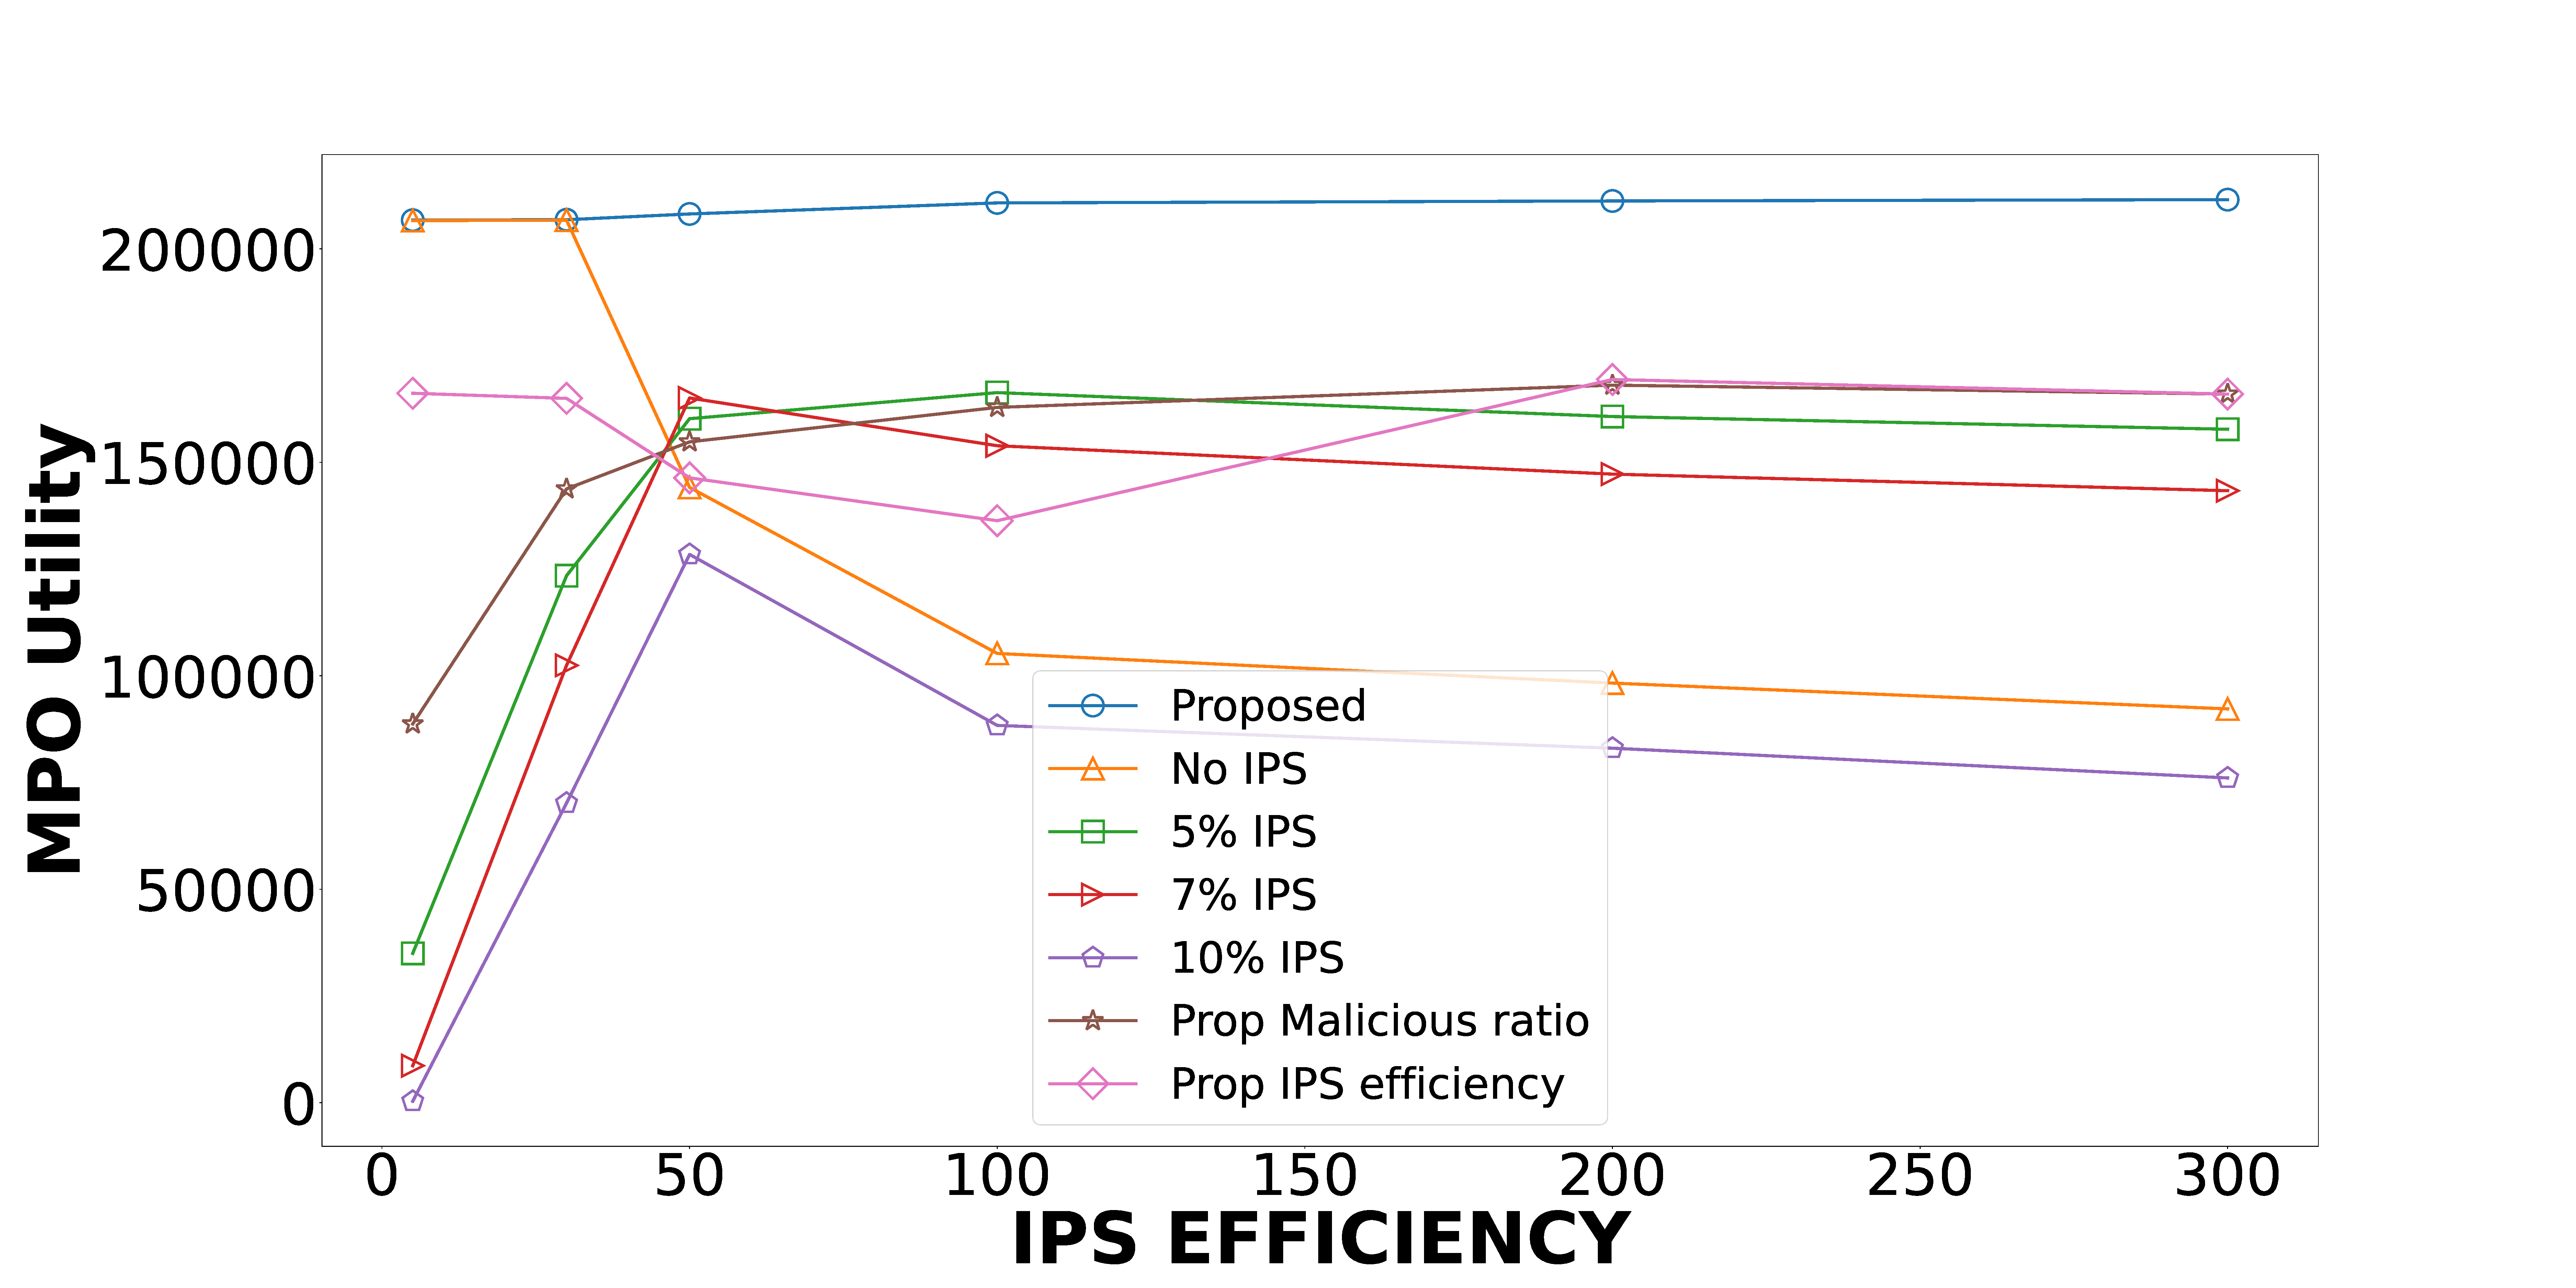
\includegraphics[width=0.33\textwidth]{5GDDoS_Game_MPO_efficiency_high_cvx.pdf}}
\label{fig:eff_high}
\caption{Different IPS efficiency of High Workload EUs}
\end{figure*}
\textbf{ASP with high workload EUs}: Similar to the case \cref{subsec:mal}, the ASPs change their best responses when the IPS efficiency increases. In the case where ASPs have high workload EUs, by \cref{eqn:service_rate}, the service rate would be low. Therefore, in this case, the interception rate would be higher than the service rate in default parameters ($\nu = 50$), and the ASPs tend to deploy more IPS VMs. However, when the IPS efficiency is low, the interception rate would be lower, and in this case, the service rate would be higher. As the efficiency of IPS increases, the best responses of the ASPs change at a specific point, which is the point where the interception rate and the service rate intersects.


When the IPS efficiency is low, the ASPs tend to deploy fewer IPS VMs. Thus, the scheme \textit{No IPS} has higher utility than \textit{5\% IPS VM} and \textit{7\% IPS VM}. When the utility of fixed ratio schemes such as \textit{5\% IPS VM} and \textit{7\% IPS VM} starts to increase because as the IPS efficiency increases, the intercepted malicious request also increases. However, the utilities of these schemes started to decrease at some point. The main reason is that, as the IPS efficiency increases, ASPs need fewer IPS VMs to defend against these attacks, and these schemes deploy redundant IPS VMs. As for \textit{10\% IPS VM}, the scheme always deploys redundant IPS VMs. Therefore, the utility is always lower than other schemes.


In \cref{fig:eff_asp_high}, as for the scheme \textit{Proportional IPS efficiency}, the utility of the scheme is higher than other scheme such as \textit{5\% IPS VM} and \textit{7\% IPS VM} when the IPS efficiency is low because it deploys less IPS VMs, which is $0.01 \times 30\% = 0.3\%$. As the IPS efficiency increases, the utility of these fixed ratio schemes \textit{5\% IPS VM} and \textit{7\% IPS VM} started to exceed the utility of \textit{Proportional IPS efficiency} because these fixed schemes deploy more IPS VMs, which can intercept more malicious requests. As the IPS efficiency increases, the utility of \textit{Proportional IPS efficiency} starts to surpass \textit{5\% IPS VM} and \textit{7\% IPS VM} because these fixed ratio scheme deploys redundant IPS VMs, and \textit{Proportional IPS efficiency} deploys the appropriate number of IPS VMs. In addition, our \textit{Proposed Scheme} has outperformed other schemes in \Cref{fig:eff_soc_high}, \Cref{fig:eff_asp_high}, and \Cref{fig:eff_mpo_high}.

% eff low
\begin{figure*}[!]
\captionsetup{justification=centering}
  \subfloat[Social Welfare\label{fig:eff_soc_low}]{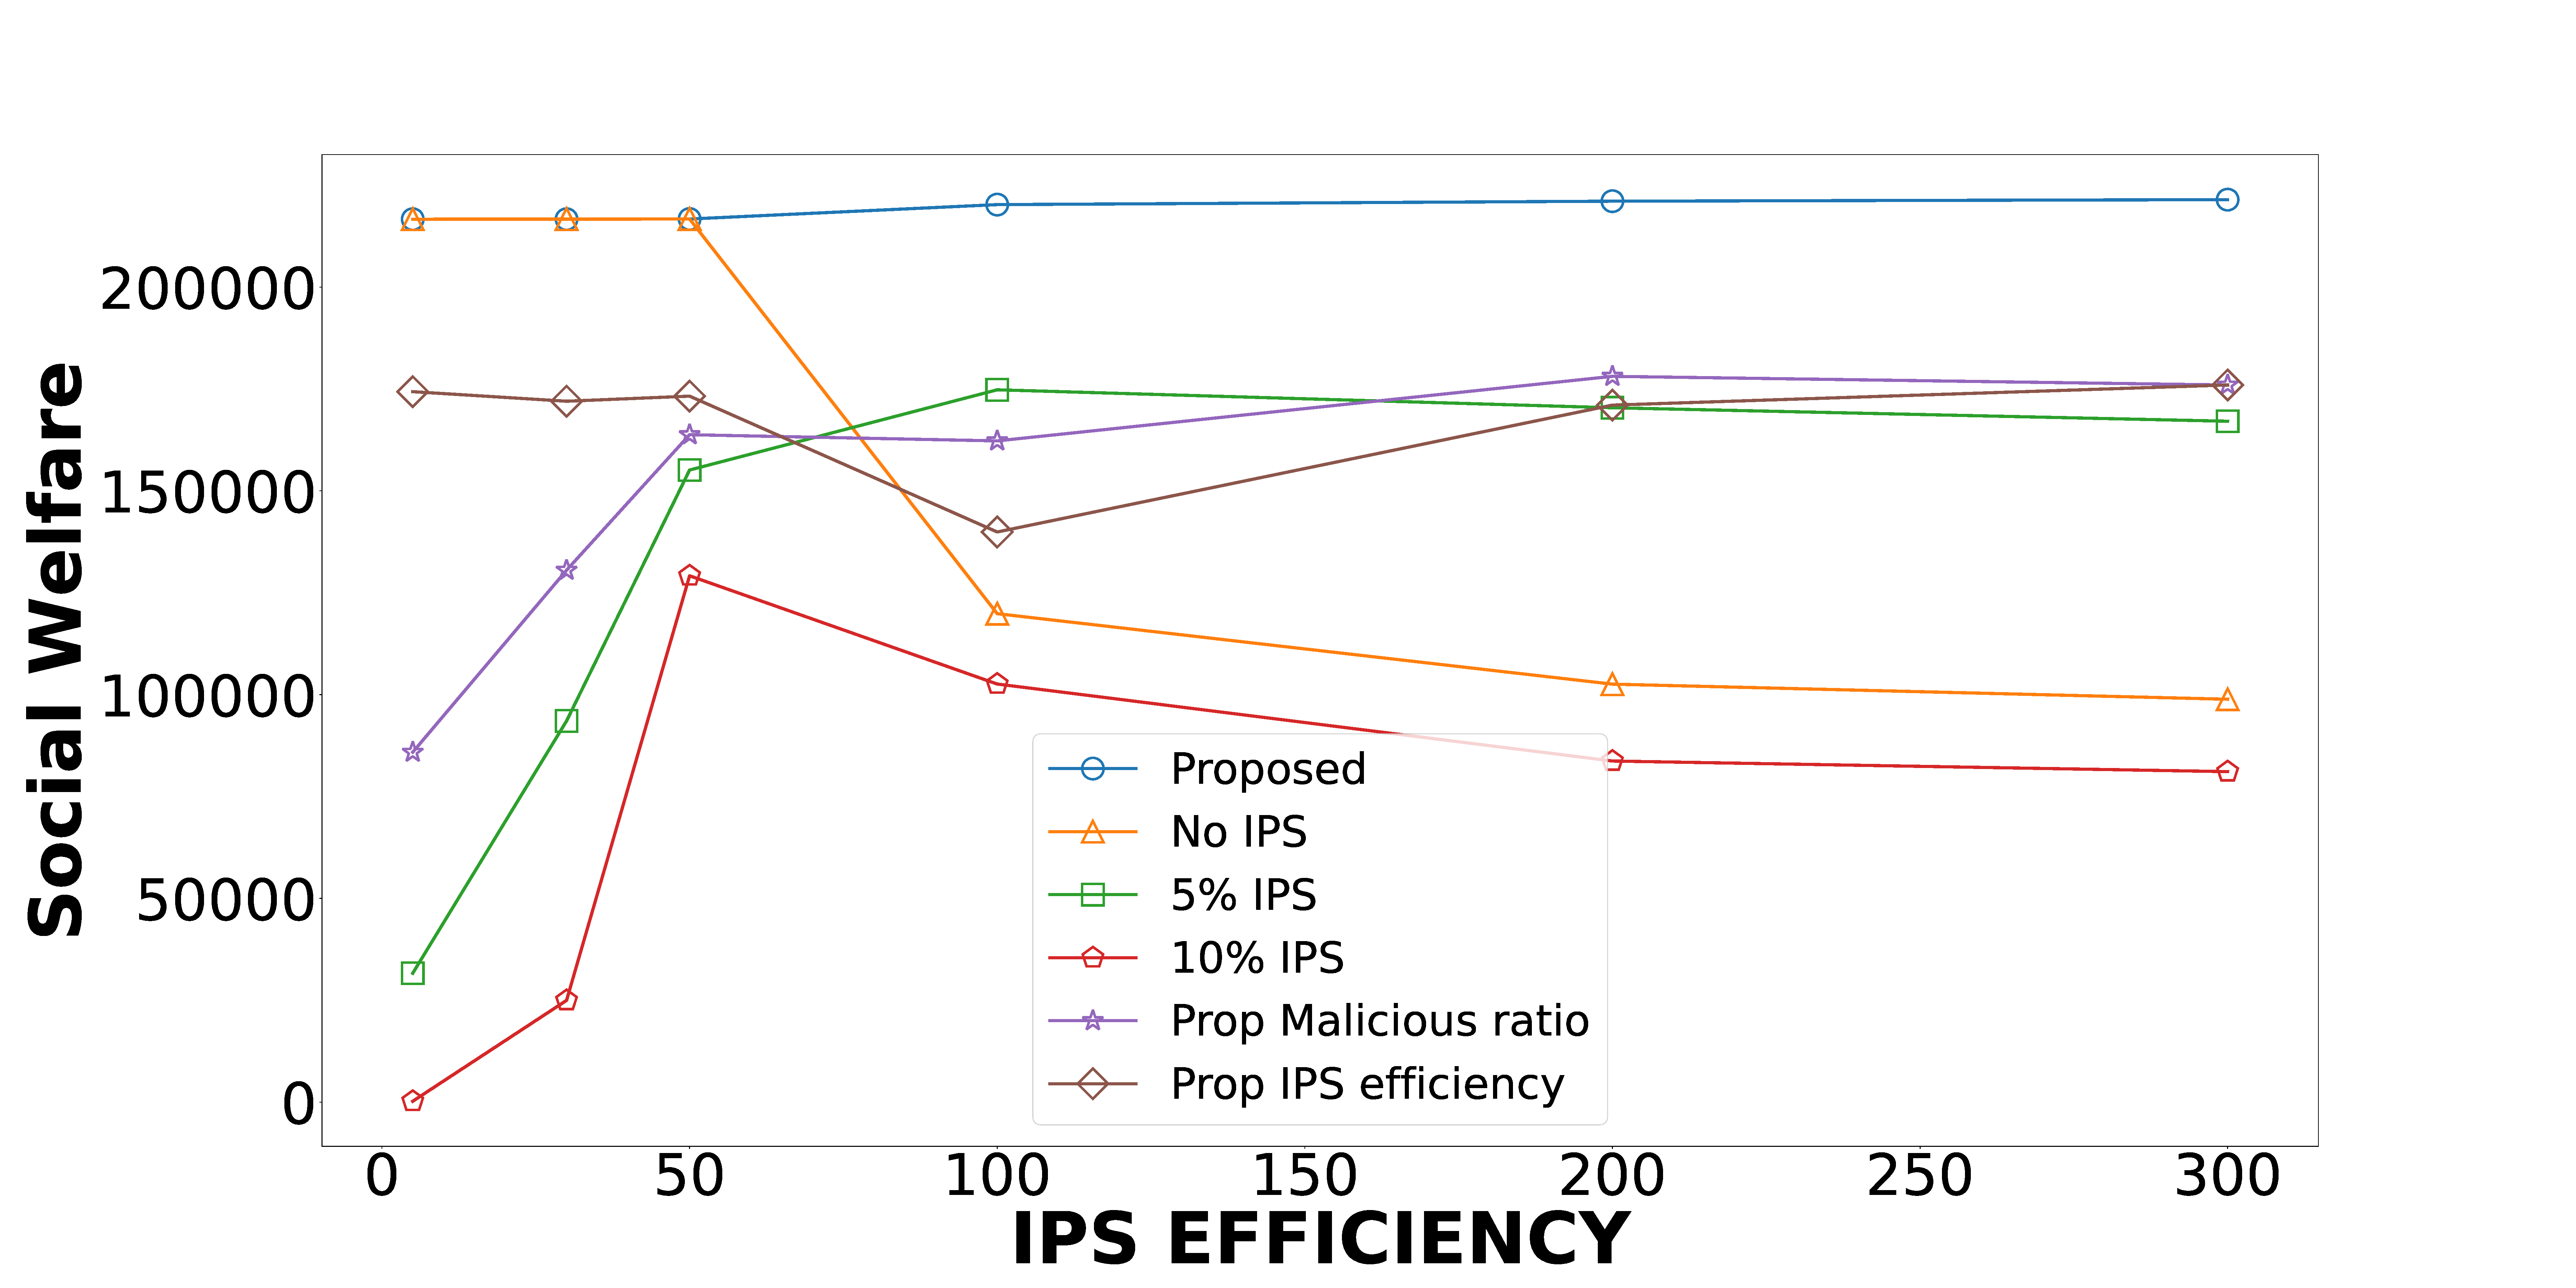
\includegraphics[width=0.33\textwidth]{5GDDoS_Game_social_efficiency_low_cvx.pdf}}
  \hfill
  \subfloat[ASP Utility\label{fig:eff_asp_low}]{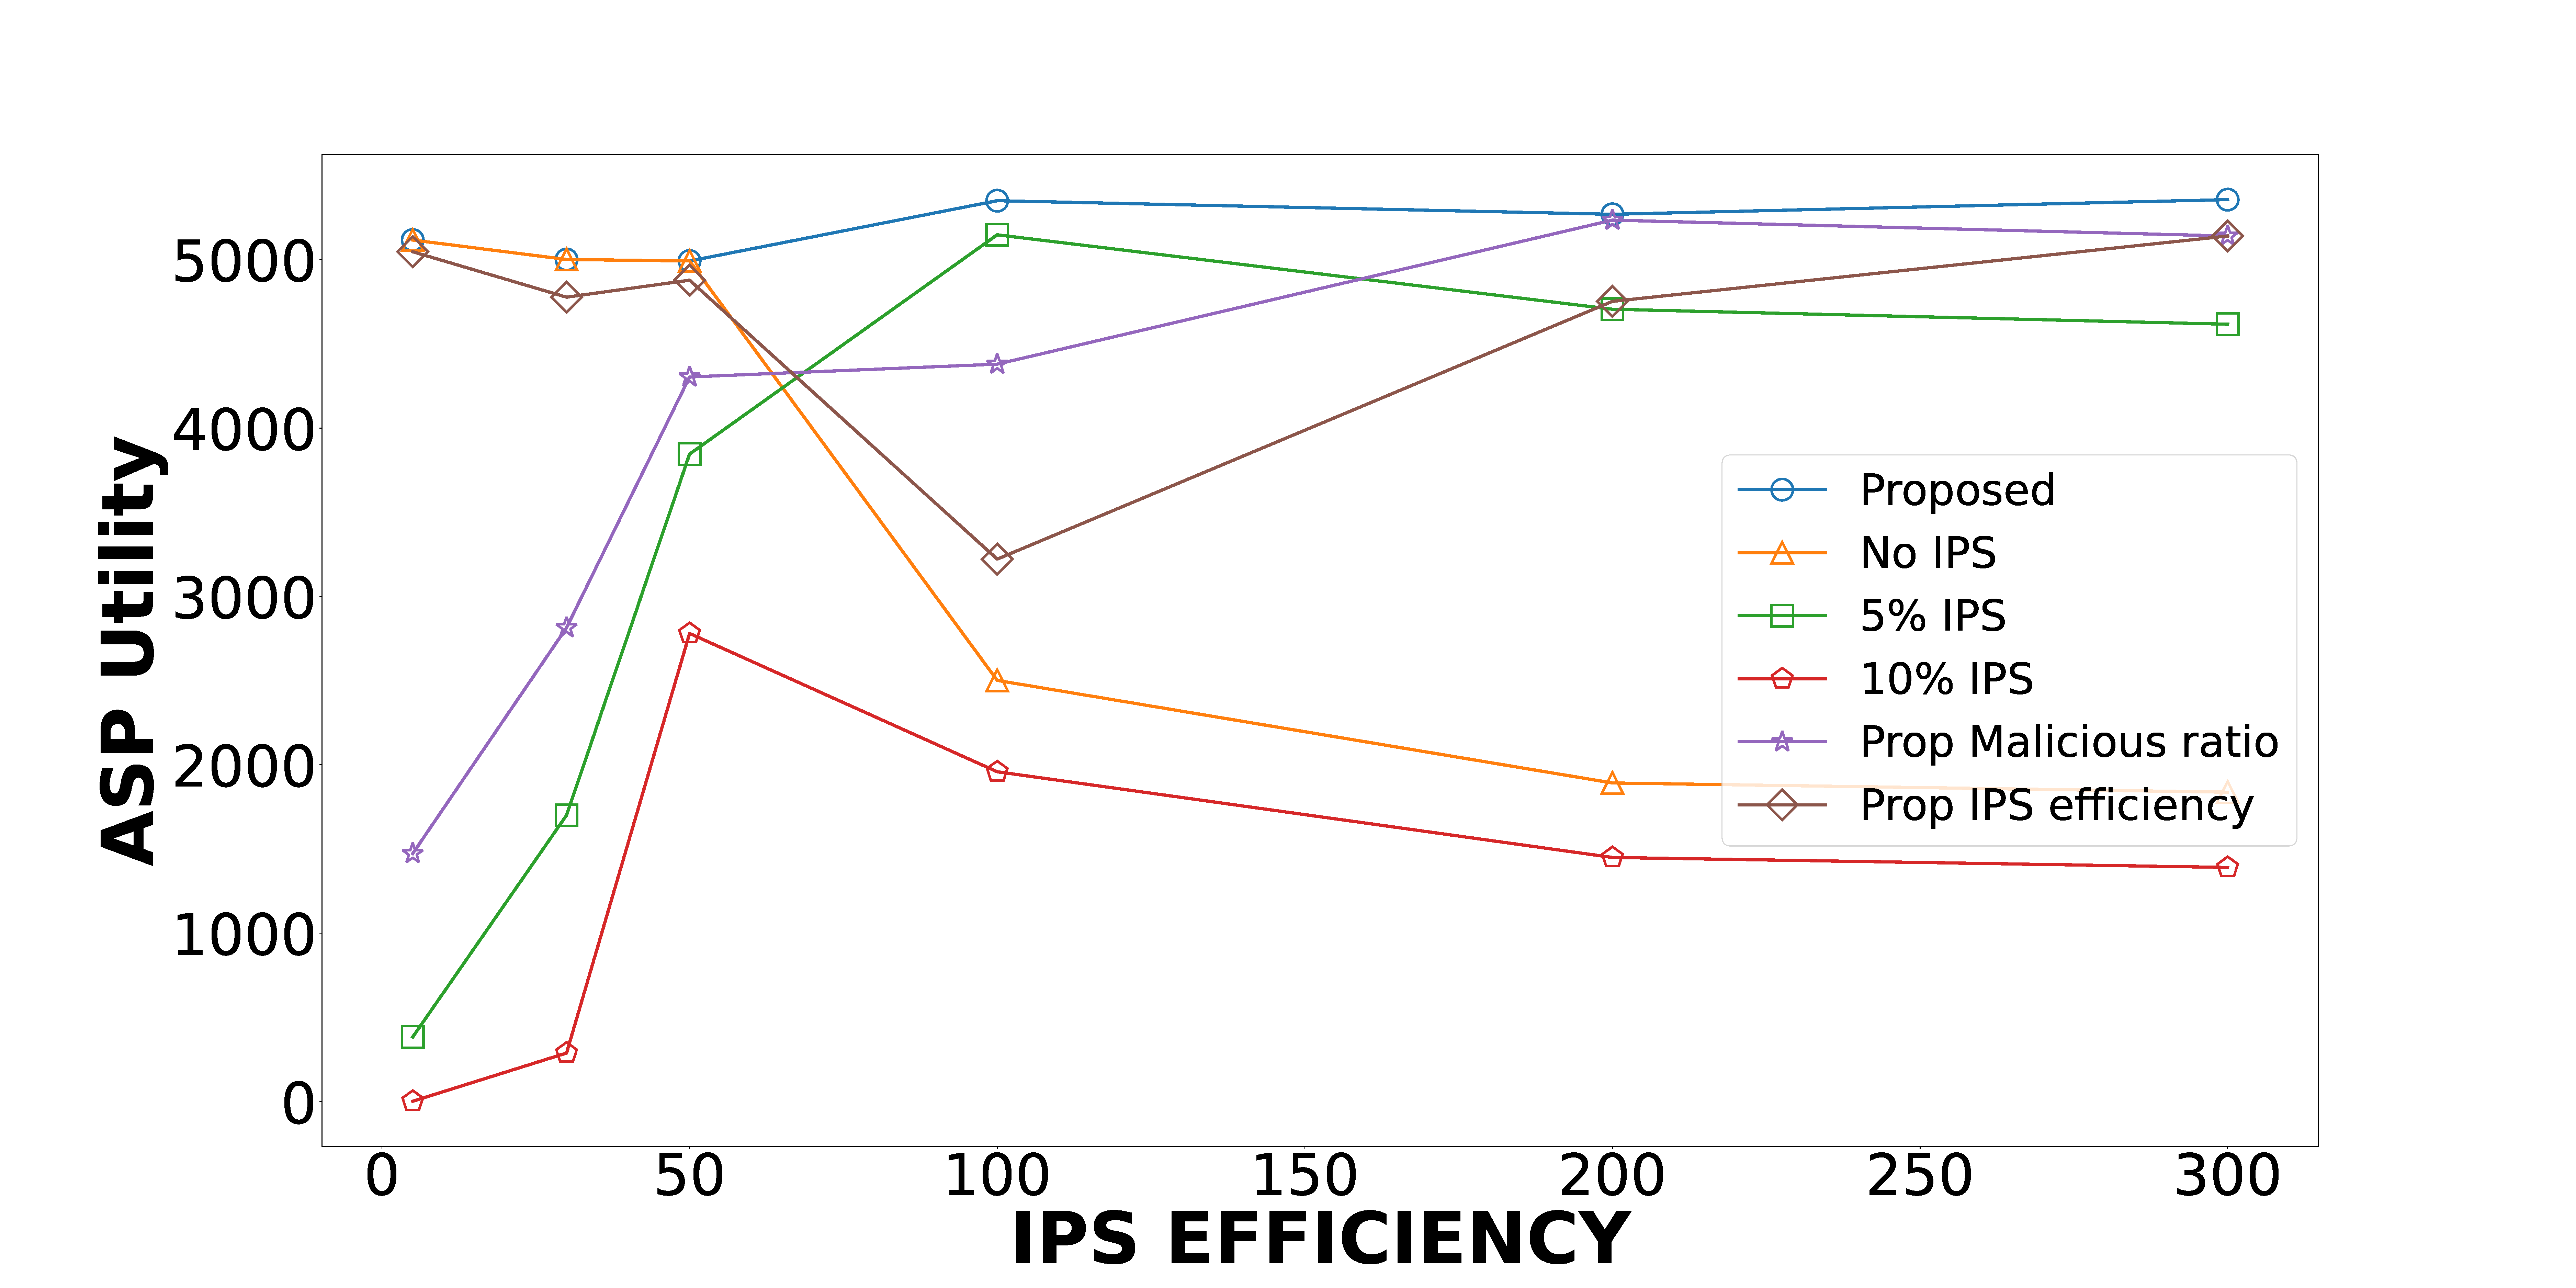
\includegraphics[width=0.33\textwidth] {5GDDoS_Game_asp_efficiency_low_cvx.pdf}}
  \hfill
  \subfloat[MPO Utility\label{fig:eff_mpo_low}]{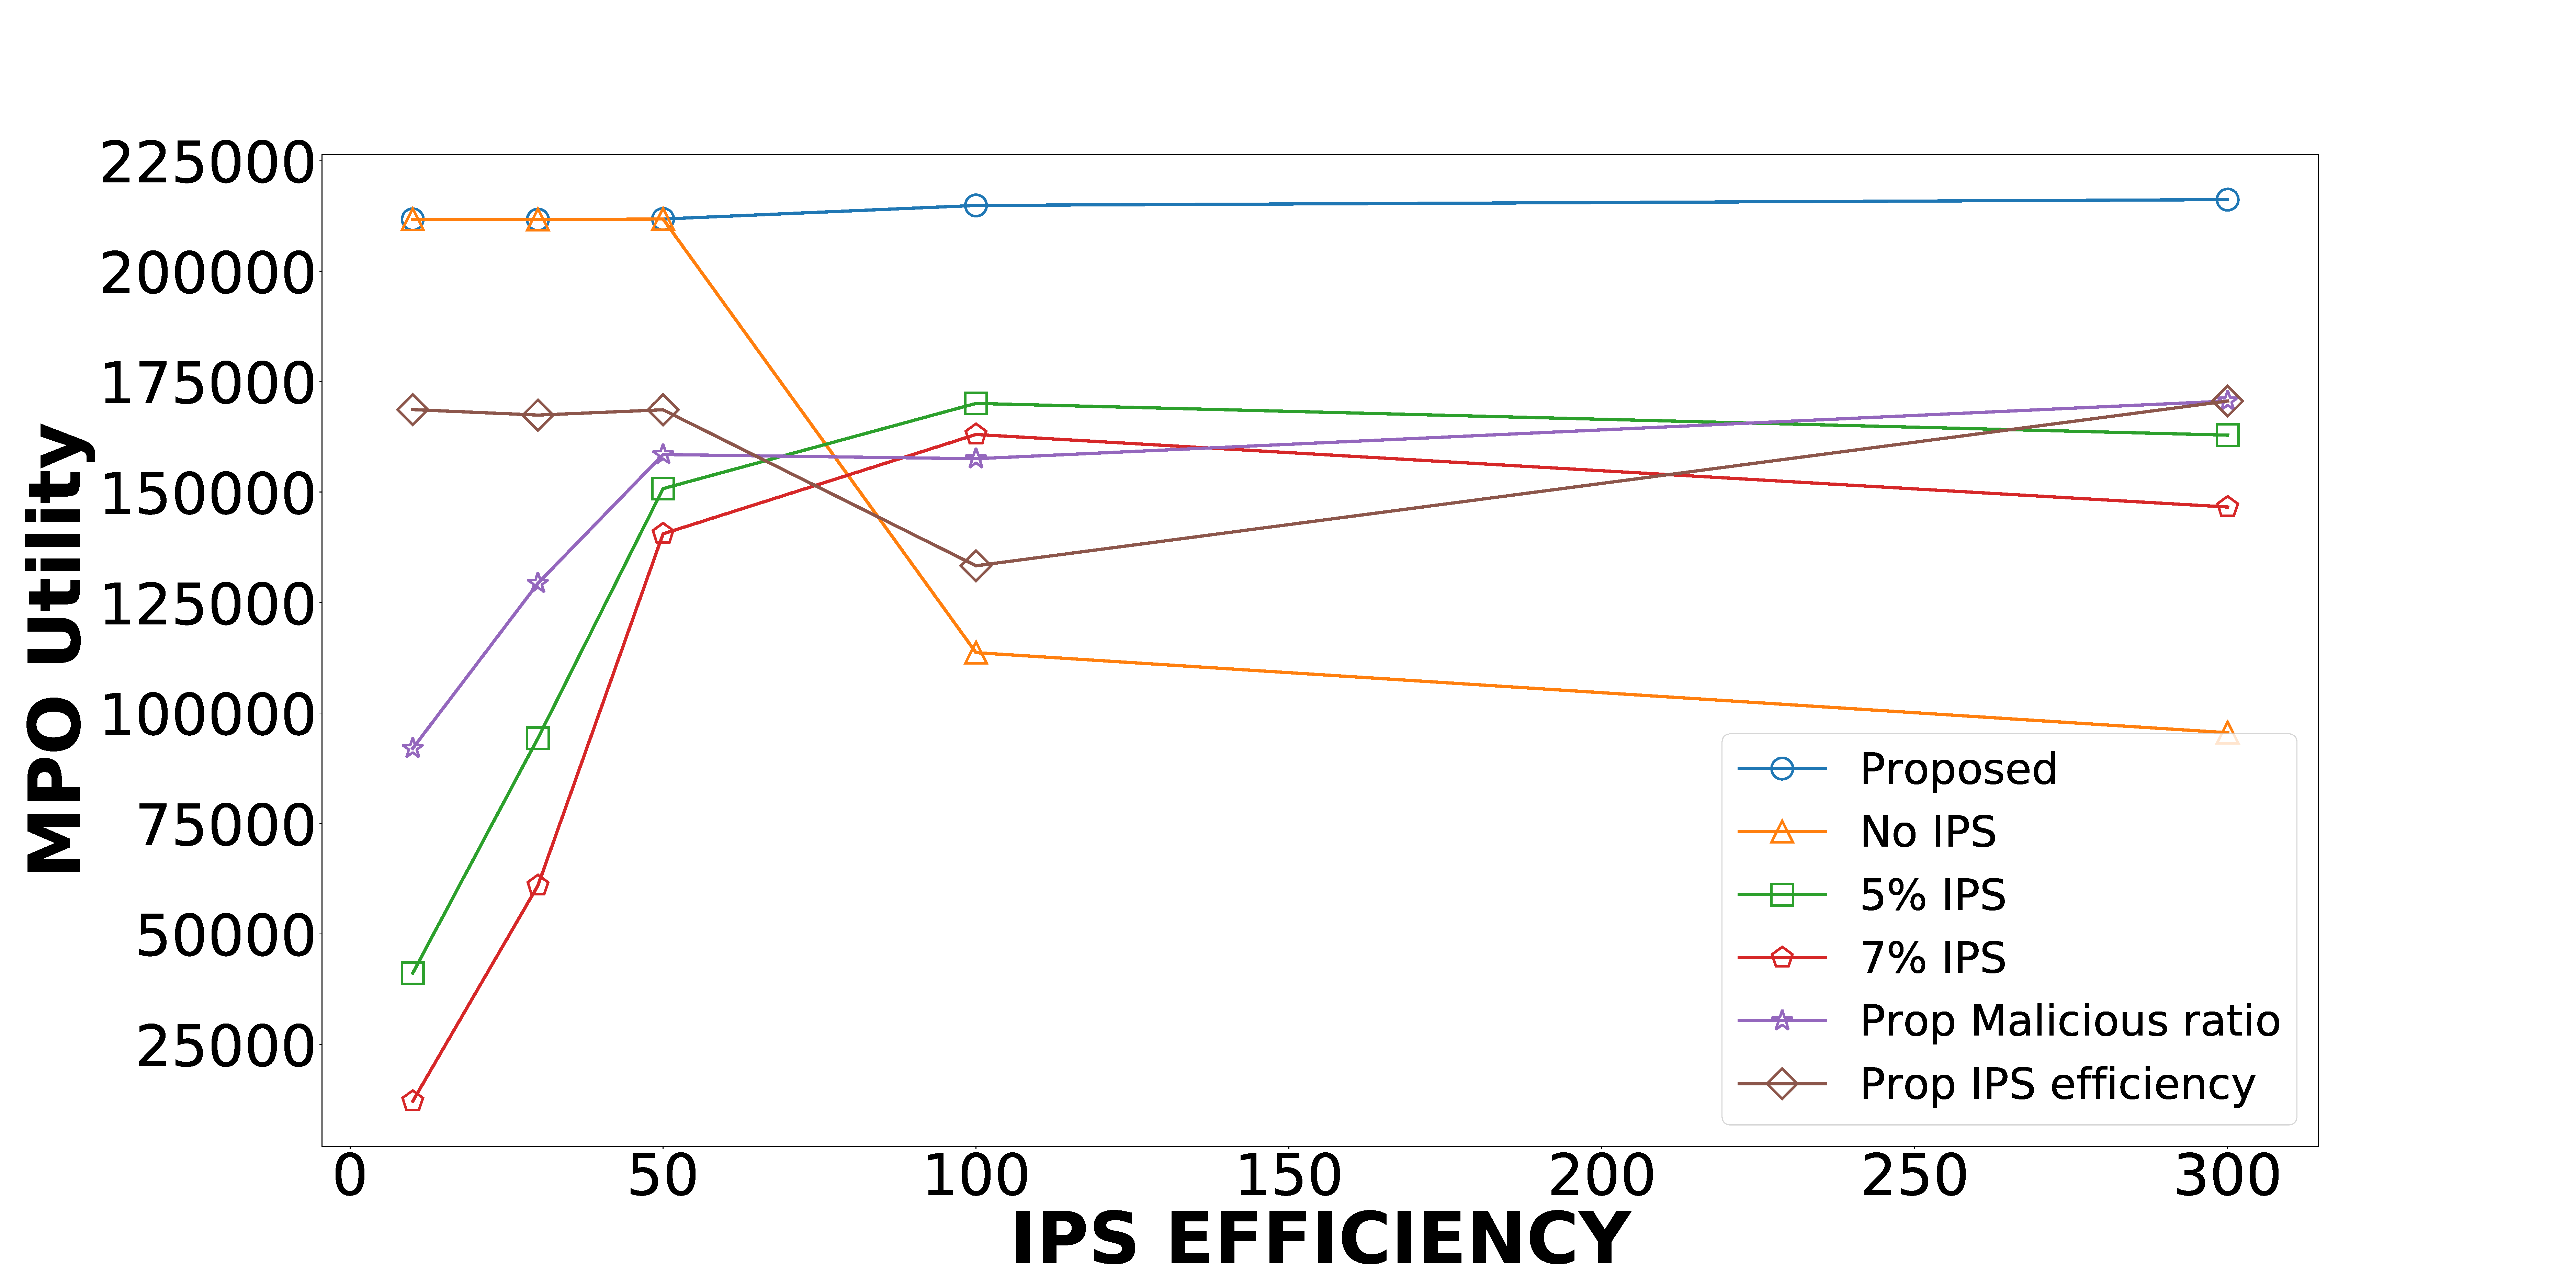
\includegraphics[width=0.33\textwidth]{5GDDoS_Game_MPO_efficiency_low_cvx.pdf}}
\label{fig:eff_low}
\caption{Different IPS efficiency of Low Workload EUs}
\end{figure*}

\textbf{ASP with low workload EUs}: In the case where ASPs have low workload EUs, by \cref{eqn:service_rate}, the service rate would be high. Therefore, the interception rate would be lower than the service rate in default parameters ($\nu = 50$), and the ASPs tend to deploy fewer IPS VMs. As the efficiency of IPS increases, the best responses of the ASPs change at a specific point, which is the point where the interception rate and the service rate intersects. The main difference with the high-workload case is that the interception rate and the service rate intersects at a point where the IPS efficiency is higher. Other than the difference previously mentioned, this case is similar to the high-workload case.
% \textcolor{blue}{We omit the figure due to page limitations.}

% \textcolor{red}{
% Similar to the previous case, where the end-users have high workload tasks, the utility of fixed ratio scheme \textit{5\% IPS VM} and \textit{7\% IPS VM} has lower utility when IPS efficiency is low. When the IPS efficiency increases, the ASPs change their best responses and tend to deploy IPS VMs to intercept malicious requests. The changes in the utility curve are similar to the previous case. To elaborate, the utility of fixed ratio schemes \textit{5\% IPS VM} and \textit{7\% IPS VM} first exceed the utility of \textit{Proportional IPS efficiency}, and when the IPS efficiency increases, the utility of \textit{Proportional IPS efficiency} exceed these fixed ratio schemes \textit{5\% IPS VM} and \textit{7\% IPS VM} again. In addition, the \textit{Proposed Scheme} outperformed other schemes in \Cref{fig:eff_soc_low}, \Cref{fig:eff_asp_low}, and \Cref{fig:eff_mpo_low} with various IPS efficiency due to the optimal IPS deployment.}

\section{Conclusion} \label{sec:conclusion}
In the paper, we proposed a flexible IPS deployment strategy for ASPs to allocate VM resources for IPS and services to mitigate the expected DDoS attacks. The joint optimization problem of ASP and MPO is formulated as a Stackelberg game to capture the hierarchy relationship. The optimal pricing strategy of MPO, the optimal number of purchased VMs, and the ratio of IPS VM for ASPs are derived. The Stackelberg equilibrium can then be derived through the proposed algorithm. The simulation results verify the effectiveness of the proposed solution in maintaining the service quality and social welfare compared with other baseline schemes.


\bibliographystyle{IEEEtran}
\bibliography{5GDDoS_Game}
\begin{IEEEbiography}[{\includegraphics[width=1in,height=1.25in,clip,keepaspectratio]{chun_yen.jpg}}]{Chun-Yen Lee}
received the B.S. degree in electrical engineering and the minor degree in economics from National Taiwan University (NTU), Taipei, Taiwan in 2021. He is currently a research assistant with the Research Center for Information Technology Innovation, Academia Sinica. His research interests include wireless communications, game theory and network economics.
\end{IEEEbiography}


\begin{IEEEbiography}[{\includegraphics[width=1in,height=1.25in,clip,keepaspectratio]{Chia-Hung.jpg}}]{Chia-Hung Lin}
received the B.S. degree in electrical engineering from National Taiwan University (NTU) in 2021. He is currently a research assistant of the Research Center for Information Technology Innovation, Academia Sinica. His research interests include wireless communications and systems.
\end{IEEEbiography}

\begin{IEEEbiography}[{\includegraphics[width=1in,height=1.25in,clip,keepaspectratio]{chang.jpg}}]{Zhan-Lun Chang}  received the BS degree in math and electrical engineering and the MS degree in electrical engineering from National Taiwan University (NTU), Taipei, Taiwan, in 2018 and 2020. His research interests include resource allocation, wireless communications, game theory, and network economics.
\end{IEEEbiography}
%
\begin{IEEEbiography}[{\includegraphics[width=1in,height=1.25in,clip,keepaspectratio]{wang.jpg}}]{Chih-Yu Wang} received the B.S. and Ph.D. degrees in electrical engineering and communication engineering from National Taiwan University (NTU), Taipei, Taiwan, in 2007 and 2013, respectively. He has been a visiting student in University of Maryland, College Park in 2011. He joined Academia Sinica, Taipei, Taiwan in 2014. He is currently an Associate Research Fellow / Associate Professor in Research Center for Information Technology Innovation. His research interests include game theory, wireless communications, social networks, and data science.

He was a recipient of the K. T. Li Young Researcher Award from ACM Taipei/Taiwan Chapter and The Institute of Information and Computing Machinery in 2019, Ministry of Science and Technology Research Project for Excellent Young Scholars in 2019. His work was featured in 2018 and 2019 Significant Research Achievements of Academia Sinica.
\end{IEEEbiography}
%
\begin{IEEEbiography}[{\includegraphics[width=1in,height=1.25in,clip,keepaspectratio]{wei.jpg}}]{Hung-Yu Wei} is a Professor in Department of Electrical Engineering and Graduate Institute of Communications Engineering, National Taiwan University. Currently, he serves as Associate Chair in Department of Electrical Engineering. He received the B.S. degree in electrical engineering from National Taiwan University in 1999. He received the M.S. and the Ph.D. degree in electrical engineering from Columbia University in 2001 and 2005 respectively. He was a summer intern at Telcordia Applied Research in 2000 and 2001. He was with NEC Labs America from 2003 to 2005. He joined Department of Electrical Engineering at the National Taiwan University in July 2005. His research interests include next-generation wireless broadband networks, IoT, fog/edge computing, cross-layer design for wireless multimedia, and game theoretic models for communications networks.

Dr. Wei received NTU Excellent Teaching Award in 2008 and 2018. He also received "Recruiting Outstanding Young Scholar Award" from the Foundation for the Advancement of Outstanding Scholarship in 2006, K. T. Li Young Researcher Award from ACM Taipei/Taiwan Chapter and The Institute of Information and Computing Machinery in 2012, Excellent Young Engineer Award from the Chinese Institute of Electrical Engineering in 2014, Wu Ta You Memorial Award from MOST in 2015, and Outstanding Research Award from MOST in 2020. He has been actively participating in NGMN, IEEE 802.16, 3GPP, IEEE P1934, and IEEE P1935 standardization. He serves as Vice Chair of IEEE P1934 Working Group to standardize fog computing and networking architecture. He serves as Secretary for IEEE ComSoC Fog/Edge Industry Community. He is an Associate Editor for IEEE System journal and IEEE IoT magazine, and was an Associate Editor for IEEE IoT journal. He is an IEEE certified Wireless Communications Professional. He was the Chair of IEEE VTS Taipei Chapter during 2016~2017. He is currently the Chair of IEEE P1935 working group for edge/fog management and orchestration standard.

\end{IEEEbiography}


\clearpage
\appendices
    \section{Proof of Lemma 1}\label{appendix:lemma_1}
    \begin{proof}
    The feasible region imposed by (\ref{eqn:asp_utility_def_opti_const1}) and (\ref{eqn:asp_utility_def_opti_const2}) is a closed and bounded interval in $\mathbb{R}$ and thus is a convex set. As the objective function (\ref{eqn:asp_utility_def_opti_obj}) is continuous in $z_i^h$, the existence of the optimal solution then comes from the Extreme Value Theorem. If (\ref{eqn:asp_utility_def_opti_obj}) is concave at each feasible $z_i^h$, optimization problem (\ref{eqn:asp_utility_def_opti}) is a convex optimization problem. It remains to show that the objective function (\ref{eqn:asp_utility_def_opti_obj}) is concave in feasible $z_i^h$. By rearranging the terms, we express $X_i(z_i^h|z_i^v,\Psi_m^v)$ as
    \begin{equation}
    \begin{aligned}
        \sum_{j \in \mathrm{U}_i^{n}}\Psi_{ij}(1-\frac{T_{ij}^t+T_i^p(z_i^v, z_i^h)-a_i}{b_i-a_i})- \Psi_m^v z_i^v 
    \end{aligned}
    \end{equation}
    To show $X_i(z_i^h|z_i^v,\Psi_m^v)$ is concave in feasible $z_i^h$, it suffices to show that $T_i^p(z_i^v, z_i^h)$ is convex in feasible $z_i^h$. We will verify the convexity of $T_i^p(z_i^v, z_i^h)$. From (\ref{eqn:asp_mm1_delay}), We can rewrite it as
    \begin{equation} 
    \begin{aligned}
    T_i^p(z_i^v)=\frac{1}{(z_i^v-z_i^h)\mu_i^v - \lambda_i + H_i(z_i^h)}
    \end{aligned}
    \end{equation}
    By definition, $H_i(z_i^h)$ is concave in feasible $z_i^h$. In addition, $(z_i^v-z_i^h)\mu_i^v - \lambda_i$ is an affine function of $z_i^h$, so $(z_i^v-z_i^h)\mu_i^v - \lambda_i + H_i(z_i^h)$ is concave in feasible $z_i^h$. Given a positive concave function $f(x)$ in feasible $x$, $\frac{1}{f(x)}$ is convex in feasible $x$. Thus, $T_i^p(z_i^v, z_i^h)$ is convex in feasible $z_i^h$ and $X_i(z_i^h|z_i^v,\Psi_m^v)$ is concave in feasible $z_i^h$.
    \end{proof}

  \section{Proof of Lemma 2}\label{appendix:lemma_2}
    \begin{proof}
    From (\ref{eqn:asp_utilitu_def_firstderiv}), we substitute $\eta_i{z_i^h}$ into $H_i(z_i^h)$, then we can obtain
    \begin{equation} \label{eqn:asp_utilitu_simplified}
    [(z_i^v - z_i^h) - \lambda_i + \eta_i{z_i^h}]^{-2} \cdot (-\mu_i^v + \eta_i)
    \end{equation}
    Obviously, regardless of the value of $z_i^h$, the (\ref{eqn:asp_utilitu_simplified}) will never be zero. Therefore, the extreme point does not exist.\qedhere
    \end{proof}

  \section{Proof of Lemma 3}\label{appendix:lemma_3}
    \begin{proof}
    If $T_{i,2}^p(z_i^v)$ is convex in feasible $z_i^v$, $Y_i^2(z_i^v|\Psi_m^v)$ is concave in feasible $z_i^v$. We will verify the convexity of $T_{i,2}^p(z_i^v)$. We can write $T_{i,2}^p(z_i^v)$ as follow
    \begin{equation} \label{eqn:asp_case2_mm1_delay_min}
    \begin{aligned}
    &T_{i,2}^p(z_i^v) = \\ &\frac{1}{(z_i^v-min(\xi_i z_i^v, \frac{\lambda_i^m}{\eta_i}))\mu_i^v - \big(\lambda_i - \eta_i\min(\xi_i z_i^v, \frac{\lambda_i^m}{\eta_i})\big)}
    \end{aligned}
    \end{equation}
    By rewriting (\ref{eqn:asp_case2_mm1_delay_min}), $T_{i,2}^p(z_i^v)$ can be further expressed as
    \begin{equation} \label{eqn:asp_case2_mm1_delay_min_new}
    \begin{aligned}
    T_{i,2}^p(z_i^v) = \frac{1}{z_i^v\mu_i^v - \lambda_i +(\eta_i - \mu_i^v)\min(\xi_i z_i^v, \frac{\lambda_i^m}{\eta_i})}
    \end{aligned}
    \end{equation}
    Since the term $(\eta_i - \mu_i^v)$ is always positive in Case 2, $(\mu_i^v - \eta_i)\min(\xi_i z_i^v, \frac{\lambda_i^m}{\eta_i})$ is positive and concave in feasible $z_i^v$. In addition, $(z_i^v\mu_i^v - \lambda_i)$ is an affine function in feasible $z_i^v$, so $z_i^v\mu_i^v - \lambda_i+(\mu_i^v - \eta_i)\min(\xi_i z_i^v, \frac{\lambda_i^m}{\eta_i})$ is concave in feasible $z_i^v$.
    
    Given a concave function $f(x)$ in feasible $x$, $\frac{1}{f(x)}$ is convex in feasible $x$. Therefore, $T_{i,2}^p(z_i^v)$ is convex in feasible $z_i^v$ and $Y_i^2(z_i^v|\Psi_m^v)$ is concave in feasible $z_i^v$.  \qedhere
    \end{proof}

  \section{Proof of Theorem 1}\label{appendix:theorem_1}
    \begin{proof}
    We begin by proving the feasible region is a convex set. $\Upsilon_i$ is a convex set because $\Upsilon_i$ is a ray starting from $\frac{\lambda_i+\gamma_i}{\mu_i^v}$ to $\infty$. Since we have proved the convexity of $Y_i^2(z_i^v|\Psi_m^v)$ in \Cref{lemma:asp_case2_utility_concave}, $\Upsilon_i^2$ is a convex set because any superlevel set of a concave function is a convex set. Since the intersection of two convex set is a convex set, $\Upsilon_i \cap \Upsilon_i^2$ is a convex set. When $\Upsilon_i \cap \Upsilon_i^2 = \emptyset$, which means the ASP $i$ cannot make the processing queue stable while has a positive utility no matter how many VMs ASP $i$ buys from the MPO. In this situation, the best action of ASP $i$ is not to buy any VM. By \Cref{lemma:asp_case2_utility_concave}, $Y_i^2(z_i^v|\Psi_m^v)$ is concave. When the extreme point of $Y_i^2(z_i^v|\Psi_m^v)$ is smaller than $\frac{\lambda_i+\gamma_i}{\mu_i^v}$, $\frac{\lambda_i+\gamma_i}{\mu_i^v}$ is the optimal point. When the extreme point of $Y_i^2(z_i^v|\Psi_m^v)$ falls in the interior of the feasible region, the extreme point is the optimal point. The extreme point of $Y_i^2(z_i^v|\Psi_m^v)$ can be solved when the first derivative of $Y_i^2(z_i^v|\Psi_m^v)$ with respect to $z_i^v$ equals zero.
    \begin{equation} \label{eqn:asp_case2_utility_first_deriv}
    -\frac{\partial T_{i,2}^p(z_i^v)}{\partial z_i^v} = \frac{\Psi_m^v (b_i - a_i)}{\sum_{j \in \mathsf{U}_i^n} \Psi_{ij}}
    \end{equation}
    Using (\ref{eqn:asp_case2_mm1_delay1}), (\ref{eqn:asp_case2_mm1_delay2}), (\ref{eqn:asp_case2_objective}), and $H_i(x)=\eta_i x$, it only takes simple algebraic operations to have the expression for the extreme point in (\ref{eqn:asp_case2_utility_extreme}). Note that since there are two kinds of $Y_i^2(z_i^v|\Psi_m^v)$ under the circumstances of (\ref{eqn:asp_case2_mm1_delay1}) and (\ref{eqn:asp_case2_mm1_delay2}), there are also two different extreme points (\ref{eqn:asp_case2_utility_extreme2_1}) and (\ref{eqn:asp_case2_utility_extreme2_2}) based on the $Y_i^2(z_i^v|\Psi_m^v)$.\qedhere
    \end{proof}
  \section{Proof of Lemma 4}\label{appendix:lemma_4}
    \begin{proof}
    If $T_{i,3}^p(z_i^v)$ is convex in feasible $z_i^v$, $Y_i^3(z_i^v|\Psi_m^v)$ is concave in feasible $z_i^v$. We can verify the convexity of $T_{i,3}^p(z_i^v)$ by taking second derivative of $T_{i,3}^p(z_i^v)$ with respect to $z_i^v$.
    
    \begin{equation} \label{eqn:asp_case3_mm1_delay_second_deriv}
    \begin{aligned}
    &[2(\mu_i^v)^2](z_i^v\mu_i^v-\lambda_i)^{-3}
    \end{aligned}
    \end{equation}
    The first term of (\ref{eqn:asp_case3_mm1_delay_second_deriv}) is positive. Moreover, $z_i^v\mu_i^v - \lambda_i$ is larger than $0$ to satisfy the constraint (\ref{eqn:asp_utility_def_opti_const1}), so the second term of (\ref{eqn:asp_utility_def_opti_const1}) is always positive. Therefore, (\ref{eqn:asp_case3_mm1_delay_second_deriv}) is non-negative, which means $T_{i,3}^p(z_i^v)$ is convex in feasible $z_i^v$. Hence, $Y_i^3(z_i^v|\Psi_m^v)$ is concave in feasible $z_i^v$. \qedhere
    \end{proof}
  \section{Proof of Theorem 2}\label{appendix:theorem_2}
    \begin{proof}
    We begin by proving the feasible region is a convex set. $\Upsilon_i$ is a convex set because $\Upsilon_i$ is a ray starting from $\frac{\lambda_i+\gamma_i}{\mu_i^v}$ to $\infty$. Since we have proved the convexity of $Y_i^3(z_i^v|\Psi_m^v)$ in \Cref{lemma:asp_case3_utility_concave}, $\Upsilon_i^3$ is a convex set because any superlevel set of a concave function is a convex set. Since the intersection of two convex set is a convex set, $\Upsilon_i \cap \Upsilon_i^3$ is a convex set. When $\Upsilon_i \cap \Upsilon_i^3 = \emptyset$, which means the ASP $i$ cannot make the processing queue stable while has a positive utility no matter how many VMs ASP $i$ buys from the MPO. In this situation, the best action of ASP $i$ is not to buy any VM. By \Cref{lemma:asp_case3_utility_concave}, $Y_i^3(z_i^v|\Psi_m^v)$ is concave. When the extreme point of $Y_i^3(z_i^v|\Psi_m^v)$ is smaller than $\frac{\lambda_i+\gamma_i}{\mu_i^v}$, $\frac{\lambda_i+\gamma_i}{\mu_i^v}$ is the optimal point. When the extreme point of $Y_i^3(z_i^v|\Psi_m^v)$ falls in the interior of the feasible region, the extreme point is the optimal point. The extreme point of $Y_i^3(z_i^v|\Psi_m^v)$ can be solved when the first derivative of $Y_i^3(z_i^v|\Psi_m^v)$ with respect to $z_i^v$ equals zero.
    \begin{equation} \label{eqn:asp_case3_utility_first_deriv}
    -\frac{\partial T_{i,3}^p(z_i^v)}{\partial z_i^v} = \frac{\Psi_m^v (b_i - a_i)}{\sum_{j \in \mathsf{U}_i^n} \Psi_{ij}}
    \end{equation}
    Using (\ref{eqn:asp_case3_mm1_delay}), (\ref{eqn:asp_case3_objective}), and $H_i(x)=\eta_i x $, it only takes simple algebraic operations to have the expression for the extreme point in (\ref{eqn:asp_case3_utility_extreme}). \qedhere
    \end{proof}
  \section{Proof of Theorem 3}\label{appendix:theorem_3}
    \begin{proof}
    We start by proving that $\sum_{i \in \mathcal{I}} (z_{i}^v(\Psi_m^v))^*$ is convex in $\Psi_m^v$ when $\Psi_m^v \in \mathcal{M}^k,\, \forall k \in \mathcal{I}$. In (\ref{eqn:total_number_VM}), the second, third and fourth term pertains to $\Psi_m^v$. As the summation of convex function is also a convex function, it suffices to prove that $(z_{i,2}^{v,e''}(\Psi_m^v))^*$ is convex in $\Psi_m^v$ for $i \in \Omega_2^{k,e''}$, $(z_{i,2}^{v,e'}(\Psi_m^v))^*$ is convex in $\Psi_m^v$ for $i \in \Omega_2^{k,e'}$ and $(z_{i,3}^{v,e}(\Psi_m^v))^*$ is convex in $\Psi_m^v$ for $i \in \Omega_3^{k,e}$. Taking the second derivative of (\ref{eqn:asp_case2_utility_extreme2_1}) and (\ref{eqn:asp_case2_utility_extreme2_2}) with respect to $\Psi_m^v$, we have
    \begin{equation}
    \frac{3}{4}(\Psi_m^v)^{-5/2}\sqrt{\frac{\sum_{j \in \mathrm{U}_i^n}\Psi_{ij}}{\mu_i^v(b_i-a_i)}} \geq 0
    \end{equation}
    \begin{equation}
    \frac{3}{4}(\Psi_m^v)^{-5/2}\sqrt{\frac{\sum_{j \in \mathrm{U}_i^n}\Psi_{ij}}{(b_i-a_i)[(1-\xi_i)\mu_i^v + \xi_i \eta_i]}} \geq 0
    \end{equation}
    In addition, take the second derivative of (\ref{eqn:asp_case3_utility_extreme}) with respect to $\Psi_m^v$, we have
    \begin{equation}
    \frac{3}{4}(\Psi_m^v)^{-5/2}\sqrt{\frac{\sum_{j \in \mathrm{U}_i^n}\Psi_{ij}}{\mu_i^v(b_i-a_i)}} \geq 0
    \end{equation}
    
    As a result, $(z_{i,2}^{v, e'}(\Psi_m^v))^*$, $(z_{i,2}^{v, e''}(\Psi_m^v))^*$ and $(z_{i,3}^{v, e}(\Psi_m^v))^*$ is convex in $\Psi_m^v \in \mathcal{M}^k,\, \forall k \in \{1,\cdots, J\}$. Since the sub-level set of a convex function is a convex set, the feasible region resulting from (\ref{eqn:f_mpo_utility_opti_const1}) is a convex set for any value $\mathcal{Q}_v$. In addition, the feasible region of (\ref{eqn:f_mpo_utility_opti_const2}) is also a convex set because the convex combination of two numbers in $\mathcal{M}^k, \forall k \in \{1, \cdots, J\}$ is still a number in $\mathcal{M}^k, \forall k \in \{1, \cdots, J\}$. Thus, the feasible region of the optimization problem (\ref{eqn:f_mpo_utility_opti}) is the intersection of two convex set and thus is a convex set. To prove that the MPO's the optimization problem (\ref{eqn:f_mpo_utility_opti}) is a convex optimization problem, what remains to do is to prove that the objective function (\ref{eqn:f_mpo_utility_opti_obj}) is concave in $\Psi_m^v \in \mathcal{M}^k,\, \forall k \in \{1,\cdots, J\}$. Using (\ref{eqn:asp_case2_utility_extreme}), (\ref{eqn:asp_case3_utility_extreme}) and (\ref{eqn:total_number_VM}), we can unfold the first term in (\ref{eqn:f_mpo_utility_opti_obj}) as follows.
    \begin{equation}\label{eqn:mpo_utility_first_term}
    \begin{aligned}
    &\Psi_m^v \cdot \sum_{i \in \mathcal{I}} (z_{i}^v(\Psi_m^v))^* = \\
    &\Psi_m^v \cdot \sum_{i\in \Omega^{k,l}}\frac{\lambda_i + \gamma_i}{\mu_i^v}+
    \Psi_m^v \cdot \sum_{i\in \Omega^{k,e'}_{2}}(z_{i,2}^{v,e'}(\Psi_m^v))^* + \\
    &\Psi_m^v \cdot \sum_{i\in \Omega^{k,e''}_{2}}(z_{i,2}^{v,e''}(\Psi_m^v))^* + \Psi_m^v \cdot \sum_{i\in \Omega^{k,e}_{3}}(z_{i,3}^{v,e}(\Psi_m^v))^*
    \end{aligned}   
    \end{equation} 
    
    
    The first term in (\ref{eqn:mpo_utility_first_term}) is a linear function of $\Psi_m^v$ which is both convex and concave. The second and third term (\ref{eqn:mpo_utility_first_term}) is concave in $\Psi_m^v$. To prove these properties, we check the concavity via the second-order test. The second derivative of the second term is
    \begin{equation}
    -\frac{1}{4}(\Psi_m^v)^{-3/2}\sum_{i \in \Omega_2^{k,e'}} \sqrt{\frac{\sum_{j \in \mathrm{U}_i^n}\Psi_{ij}}{(b_i-a_i)[(1-\xi_i)\mu_i^v + \xi_i \eta_i]}} \leq 0
    \end{equation}
    The second derivative of the third term is
    \begin{equation}
    -\frac{1}{4}(\Psi_m^v)^{-3/2}\sum_{i \in \Omega_2^{k,e''}} \sqrt{\frac{\sum_{j \in \mathrm{U}_i^n}\Psi_{ij}}{\mu_i^v(b_i-a_i)}} \leq 0
    \end{equation}
    And the second derivative of the forth term is
    \begin{equation}
    -\frac{1}{4}(\Psi_m^v)^{-3/2}\sum_{i \in \Omega_3^{k,e}} \sqrt{\frac{\sum_{j \in \mathrm{U}_i^n}\Psi_{ij}}{\mu_i^v(b_i-a_i)}} \leq 0
    \end{equation}
    Therefore, (\ref{eqn:mpo_utility_first_term}) is concave in $\Psi_m^v$. The second term of (\ref{eqn:f_mpo_utility_opti_obj}), $C_m^v\big(\sum_{i \in \mathcal{I}} (z_{i}^v(\Psi_m^v)^*)$, is convex in $\Psi_m^v$ as it is a composition of $C_m^v$ and $\sum_{i \in \mathcal{I}} (z_{i}^v(\Psi_m^v))^*$ where $C_m^v$ is convex and non-decreasing, and $\sum_{i \in \mathcal{I}} (z_{i}^v(\Psi_m^v))^*$ is convex in $\Psi_m^v \in \mathcal{M}^k,\, \forall k \in \{1, \cdots, J\}$. Since a concave function minus a convex function yields a concave function, (\ref{eqn:f_mpo_utility_opti_obj}) is concave in $\Psi_m^v \in \mathcal{M}^k,\, \forall k \in \{1, \cdots, J\}$. In sum, the (\ref{eqn:f_mpo_utility_opti}) in each interval $\mathcal{M}^k, \forall k \in \{1, \cdots, J\}$ is a convex optimization problem. \qedhere
    \end{proof}
  \section{Proof of Theorem 4}\label{appendix:theorem_4}
    \begin{proof}
    In Case 2, we have analytical solutions for ASPs' optimal number of VMs to buy from the MPO by \Cref{thm:asp_case2_optimal}. The best response sets for ASPs defined in (\ref{eqn:asp_best_response}) are non-empty. Also, in Case 3, we have analytical solutions for ASPs' optimal number of VMs to buy from the MPO by \Cref{thm:asp_case3_optimal}. The best response sets for ASPs defined in (\ref{eqn:asp_best_response}) are non-empty. 
    
    With the optimal responses from the ASPs, the MPO's optimal price per VM $\Psi_m^v$ exists because MPO's optimization problem is convex proved in \Cref{thm:f_mpo_convex_optimization} with a compact region; thus, the MPO's best response set defined in (\ref{eqn:mpo_best_response}) is non-empty. By \Cref{def:stackelberg_equilibrium}, there is at least one Stackelberg game equilibrium.
    \end{proof}
\end{document}